%% RiSE Latex Template - version 0.5
%%
%% RiSE's latex template for thesis and dissertations
%% http://risetemplate.sourceforge.net
%%
%% (c) 2012 Yguaratã Cerqueira Cavalcanti (yguarata@gmail.com)
%%          Vinicius Cardoso Garcia (vinicius.garcia@gmail.com)
%%
%% This document was initially based on UFPEThesis template, from Paulo Gustavo
%% S. Fonseca.
%%
%% ACKNOWLEDGEMENTS
%%
%% We would like to thanks the RiSE's researchers community, the 
%% students from Federal University of Pernambuco, and other users that have
%% been contributing to this projects with comments and patches.
%%
%% GENERAL INSTRUCTIONS
%%
%% We strongly recommend you to compile your documents using pdflatex command.
%% It is also recommend use the texlipse plugin for Eclipse to edit your documents.
%%
%% Options for \documentclass command:
%%         * Idiom
%%           pt   - Portguese (default)
%%           en   - English
%%
%%         * Text type
%%           bsc  - B.Sc. Thesis
%%           msc  - M.Sc. Thesis (default)
%%           qual - PHD qualification (not tested yet)
%%           prop - PHD proposal (not tested yet)
%%           phd  - PHD thesis
%%
%%         * Media
%%           scr  - to eletronic version (PDF) / see the users guide
%%
%%         * Pagination
%%           oneside - unique face press
%%           twoside - two faces press
%%
%%		   * Line spacing
%%           singlespacing  - the same as using \linespread{1}
%%           onehalfspacing - the same as using \linespread{1.3}
%%           doublespacing  - the same as using \linespread{1.6}
%%
%% Reference commands. Use the following commands to make references in your
%% text:
%%          \figref  -- for Figure reference
%%          \tabref  -- for Table reference
%%          \eqnref  -- for equation reference
%%          \chapref -- for chapter reference
%%          \secref  -- for section reference
%%          \appref  -- for appendix reference
%%          \axiref  -- for axiom reference
%%          \conjref -- for conjecture reference
%%          \defref  -- for definition reference
%%          \lemref  -- for lemma reference
%%          \theoref -- for theorem reference
%%          \corref  -- for corollary reference
%%          \propref -- for proprosition reference
%%          \pgref   -- for page reference
%%
%%          Example: See \chapref{chap:introduction}. It will produce 
%%                   'See Chapter 1', in case of English language.

\RequirePackage{risethesis/psboxit}
\documentclass[en,oneside,onehalfspacing,msc]{risethesis/risethesis}

\usepackage[english]{babel}
\usepackage{colortbl}
\usepackage{color}
\usepackage[table]{xcolor}
\usepackage{microtype}
\usepackage{bibentry}
%\usepackage{subfigure}
\usepackage{multirow}
\usepackage{rotating}
\usepackage{booktabs}
\usepackage{pdfpages}
\usepackage{caption}
\usepackage{lipsum}
\usepackage{algorithm}
\usepackage{algpseudocode}
\usepackage{subcaption}

\captionsetup[table]{position=top,justification=centering,width=.85\textwidth,labelfont=bf,font=small}
\captionsetup[lstlisting]{position=top,justification=centering,width=.85\textwidth,labelfont=bf,font=small}
\captionsetup[figure]{position=bottom,justification=centering,width=.85\textwidth,labelfont=bf,font=small}

%% Change the following pdf author attribute name to your name.
\usepackage[linkcolor=black,
            citecolor=black,
            urlcolor=black,
            colorlinks,
            pdfpagelabels,
            pdftitle={Thiago Lacerda M.Sc. Thesis},
            pdfauthor={Thiago de Barros Lacerda}]{hyperref}

\usepackage{mathtools}
\DeclarePairedDelimiter\floor{\lfloor}{\rfloor}

% So the risethesis template can find the cinlogo image
\graphicspath{{risethesis/}}

\address{RECIFE}

\universitypt{Universidade Federal de Pernambuco}
\universityen{Federal University of Pernambuco}

\departmentpt{Centro de Informática}
\departmenten{Informatics Center}

\programpt{Pós-graduação em Ciência da Computação}
\programen{Post Graduation in Computer Science}

\majorfieldpt{Ciência da Computação}
\majorfielden{Computer Science}

\title{Some Title Related to Fast Flock Detection Algorithm}

\date{2016}

\author{Thiago de Barros Lacerda}
\adviser{Stênio Flávio de Lacerda Fernandes}

% Macros (defines your own macros here, if needed)
\def\x{\checkmark}

\begin{document}

\frontmatter

\frontpage

\presentationpage

\begin{fichacatalografica}
	\FakeFichaCatalografica % Comment this line when you have the correct file
%     \includepdf{fig_ficha_catalografica.pdf} % Uncomment this
\end{fichacatalografica}

\banca

\begin{dedicatory}
I would like to deeply thank my supervisor and God, which are basically the same!
\end{dedicatory}

\acknowledgements
To be honest, I thought that would not finish this. I was already seeing myself giving up this masters due to a lot of
things: new country, new city, new job, huge load of work in my new job, baby coming... etc.. It was not easy to work on
double journey for lots of months, sleeping only 3 to 4 hours a day. But yes! It is over! Some people helped me to no
give up and keep up with that "stressful journey" and here they deserve my "Thank you!".

I would like to thank my advisor Stênio, by having me as his student, for the second time, and lending me some time of
his busy agenda, helping me out to finish this work.

Many thanks to my beloved wife, who was always supporting me during the years of this masters, telling me to never give
up and giving up time with me in favor of me working on this dissertation. Also, thanks to my baby boy Daniel, who isn't
even born yet, but helped me to finish this dissertation as fast as possible so I can enjoy some free time before I lose
them all after he is born :). Thanks to my mother Catari and my father Cândido for their support during this time too.

Thanks to Andre, who was always telling me that we were going to end this and was also always warning me about the
important deadline dates of the University. I also would like to thank my friends here in Seattle: PP and Fabio, for
lending me some VMs on their Azure accounts, so I could run my benchmarks; Fernando, for good academic advices and
motivational speechs :).



\begin{epigraph}[]{Tiririca}
Quem é você?
\end{epigraph}

\resumo
% Escreva seu resumo no arquivo resumo.tex
Detecção de padrões em dados espaço-temporais tem se mostrado um tema de muita relevância nos dias atuais, tanto na
academia quanto na indústria, devido a sua vasta aplicabilidade em auxiliar a solucionar problemas enfrentados na
sociedade. Muitos desses problemas podem ser classificados no conexto de Cidades Inteligentes (\textit{Smart Cities}),
como Gerenciamento de Tráfego, Segurança e Planejamento de Cidades. Dentre os vários padrões espaço-temporais que podem
ser extraídos de uma base de dados, o padrão de \textit{flock} é um que vem atraindo muita atenção, devido a sua relação
intrínseca com os problemas mencionados anteriormente. Muitas pesquisas vêm sendo feitas academia, visando desenvolver
algoritmos capazes de identificar o padrão de \textit{flock}. Porém, nenhum deles foi capaz de executar tal tarefa
eficientemente, nem conseguiu escalar de maneira aceitável quando uma base de dados de grande tamanho foi analisada.
Além disso, não foi encontrado nos trabalhos relacionados uma arquitetura de \textit{software} que conseguisse ser
simples e extensível o suficiente para ser usada nos vários problemas de detecção de padrões em dados espaço-temporais.
Com isso em mente, essa dissertação propõe uma Arquitetura de \textit{Software} que pode ser usada como base para
solucionar um grande número de problemas relacionados a mineração de padrões em dados espaço-temporais. Tal arquitetura
foi então usada como base na implementação de um algoritmo de detecção de \textit{flock}, focando em alcançar grandes
ganhos em tempo de processamento, sem comprometer a precisão, visando então cenários de aplicações de tempo real em
Cidades Inteligentes. No fim, nós propomos uma remodelagem no nosso algoritmo para poder utilizar ao máximo o poder de
processamento oferecido pelas arquiteturas Multi-core dos processadores modernos. Nossos resultados mostraram que nossa
solução conseguiu superar propostas do estado da arte, alcançando 99\% de redução no tempo de processamento total. Além
disso, nossa remodelagem \textit{multi-thread} conseguiu melhorar os resultados da nossa solução em até 96\% em alguns
casos. A eficiência e performance da nossa proposta foi comprovada com avaliações feitas com bases de dados geradas
sinteticamente e coletadas em experimentos reais.

\begin{keywords}
Cidades Inteligentes, Mineração de Padrões, Dados Espaço-temporais, Padrão de Flock
\end{keywords}


\abstract
% Write your abstract in a file called abstract.tex
Pattern mining in spatio-temporal datasets is a really relevant subject in the academia and the industry nowadays, due
to its wide applicability in helping to solve real world problems. Many of them can be found in the context of Smart
Cities, like Traffic Management, Surveillance and Security and City Planning, to name a few. Among the various
spatio-temporal patterns that one can extract from a spatio-temporal dataset, the flock pattern is one that has gained a
lot of attention, because of its intrinsic relation with the aforementioned problems. A lot of work has been done in the
academia, in order to provide algorithms able to identify the flock pattern. However, none of them could perform that
task efficiently nor be able to scale well when a large dataset was the analysis target. Additionally, we found that
there was no System Architecture proposal that could be simple and extensible enough to be used in the various
spatio-temporal pattern detection problems present today. Given that context, this dissertation proposes a Generic
System Archicture that can be used to solve a great number of spatio-temporal pattern mining problems. We then validate
such architecture by implementing on top of it an efficient flock detection algorithm, aiming at achieving considerable
gains in execution time without compromising accuracy, thus targeting real-time deployment and online processing in
Smart Cities. Last, but not least, we remodel our algorithm in order to take advantage of multi-core architectures
present in modern computers. Our results indicate that our proposal outperforms the current state-of-the-art techniques,
by achieving 99\% CPU time improvement. Moreover, with our multi-thread model, we were able to reduce the processing
time of our proposed algorithm by 96\% in some cases. We prove the efficiency of our solution by performing evaluation
with both real and synthetic large datasets.

\begin{keywords}
Smart Cities, Pattern Mining, Spatio-temporal data, Flock Pattern
\end{keywords}


% List of figures
\listoffigures

% List of tables
\listoftables

% List of acronyms
% Acronyms manual: http://linorg.usp.br/CTAN/macros/latex/contrib/acronym/acronym.pdf
\listofacronyms
\begin{acronym}[ACRONYM]
% Change the word ACRONYM above to change the acronym column width.
% % The column width is equals to the width of the word that you put.
% % Read the manual about acronym package for more examples:
% %   http://linorg.usp.br/CTAN/macros/latex/contrib/acronym/acronym.pdf
\acro{aws}[AWS]{Amazon Web Services}
\acro{bfe}[BFE]{Basic Flock Evaluation}
\acro{bitdf}[BitDF]{Bitmaps for Disk Filtering}
\acro{cpu}[CPU]{Central Processing Unit}
\acro{dc}[DC]{Dynamic Convoy}
\acro{dd}[DD]{Data Decoder}
\acro{dl}[DL]{Data Listener}
\acro{dp}[DP]{Data Processor}
\acro{dsc}[DSC]{Data Source Connector}
\acro{ec}[EC]{Evolving Convoy}
\acro{egc}[EGC]{Extended Grid Cell}
\acro{fp}[FP]{Flock Processor}
\acro{gps}[GPS]{Global Positioning System}
\acro{gsb}[GSB]{GPS Stream Buffering}
\acro{ibmc}[IBMC]{Influence-based Moving Cluster}
\acro{iot}[IoT]{Internet of Things}
\acro{lts}[LTS]{Long Term Support}
\acro{mfp}[MFP]{Maximal-duration Flock Pattern}
\acro{mo}[MO]{Moving Object}
\acro{mt}[MT]{Multi-thread}
\acro{pfp}[PFP]{Parallel Flock Processor}
\acro{remo}[REMO]{RElative MOtion}
\acro{dbscan}[DBSCAN]{Density-based Spatial Clustering of Applications with Noise}
\acro{wgs84}[WGS84]{World Geodetic System 1984}
\acro{whoi}[WHOI]{Wooods Hole Oceanographic Institution}
\end{acronym}


% Summary (tables of contents)
\tableofcontents

\mainmatter

\chapter{Introduction}
\label{chp:introduction}
The advances of positioning technologies are empowering a myriad of different objects present in our daily usage, e.g.
vehicles, smartphones and wearable devices, to be shipped with location tracking systems. Those devices are able to
collect and report mobility information of people, animals and natural phonemena (e.g. hurricanes), to name a few. That
technological advance is enabling the generation of massive volumes of spatio-temporal data that can contain information
ranging from the daily routine of residents of a city \citep{whatdidyoudo} to behaviors of wild animals in a specific
region \citep{trajclustering}\citep{miningperiodic}. It is notorious the interest of the academy in such subject,
specially with the rising of Smart Cities, in which spatio-temporal datasets can provide important insights in the
context of traffic management and urban planning \citep{gissmartcities}\citep{parallelsmartcities}. Those datasets can
be used to help solving a variety of problems and answer questions, such as:

\begin{enumerate}
    \item \textbf{What are the busiest times and locations (such as traffic jams locations) in a city?}
        \citep{visualtrafficjam}
    \item \textbf{What is the movement patterns of the citizens of a city during work hours?}
    \item \textbf{What is the migration pattern of inhabitants of a specific area?}
    \item \textbf{What is the movement behavior of wild animals in their habitat?} \citep{movemine}
    \item \textbf{Is there any suspicious movement of groups o objects during that time window?}
\end{enumerate}

That list can grow indefinitely, as the scenarios and applications of spatio-temporal data analysis is vast. Some of the
questions listed above are in the context of Smart Cities, which can take advantage of spatio-temporal data analysis as
an aid to a broad set of applications, like urban planning, public security, and public health and commerce
\citep{ieeesmartcities}. Aditionally, understanding that data and being able to take actions fast according to the
conclusions extracted from them is crucial to create and evolve a Smart City. However, due to the volume of data that is
produced on a daily basis and needs to be analyzed to in order to help those applications and answer those questions,
the main problem is still the same: how to be able to analyze massive data volumes fast and efficiently so we can
empower decision takers to act quickly?

In the aforementioned questions and applications, some of the queries are intrinsically related to collaborative or
group patterns, such as flock \citep{gudefficient}, convoy \citep{convoy}, swarm \citep{swarm}, and the like. Those
patterns contain moving objects that have a strong relationship by being close to each other, within a certain distance
range and during some minimum time interval. Due to the wide range of applicability in the scenario of Smart Cities
(e.g. city roads planning, intelligent transportation, public security, etc.), the data mining of such patterns has
gained great importance in both industry and academy. There are a number of research challenges in this topic, specially
regarding the development of accurate algorithms to detect those patterns. In addition of being precise, it is of
paramount importance to design fast algorithms so that they can be keep up with real-time data. Hence, reiterating what
as mentioned in the previous paragraph, efficiently extraction of data patterns for real-time analysis and on the fly
decision-making is still an open challenge.
% * <steniofernandes@gmail.com> 2016-05-26T15:01:34.895Z:
%
% gap: why individual tracking is not a good idea? in other words, why perform flock analysis in several contexts, including smart cities
%
% ^.

\begin{figure}[h!]
    \centering
    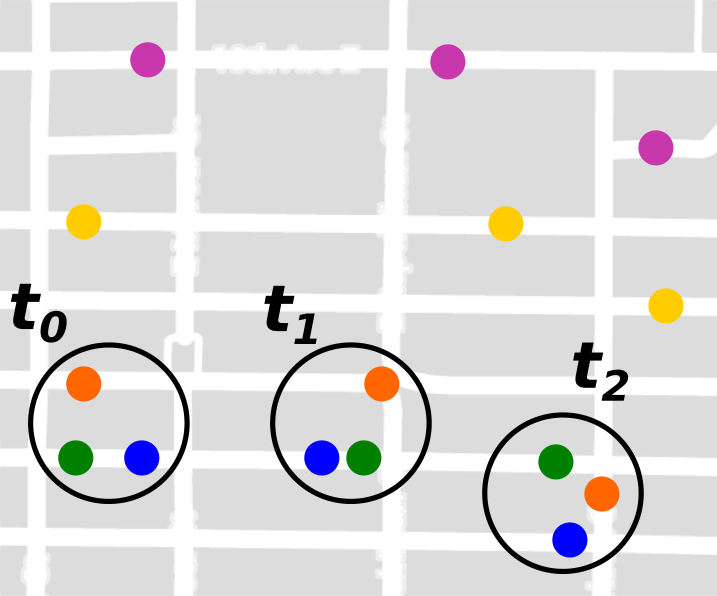
\includegraphics[width=0.7\linewidth]{images/flock_pattern.png}
    \caption{T1, T2 and T3 form a flock of size 3 with minimum length of three time steps, with a disk enclosing all
        trajectories at each time step}
    \label{fig:flocks}
\end{figure}

Among those collaborative patterns, the flock pattern is one that has gained a lot of attention in the academy, since it
can address all the scenarios and questions that were mentioned in this chapter and represents a very familiar behavior
that is frequently seen in our daily routines. A seminal formal definition of that pattern was proposed by \citep{remo}
and \citep{gudefficient} and since then, a lot of other studies has follow suit (we refer the reader to
\chapref{chp:relatedwork} for some of them), mainly due to the interests in developing mechanisms to solve real-world
problems in the scope of Internet of Things (IoT) \citep{iot} and Smart Cities \citep{smartcities}.  According to
\citep{gudefficient}, a flock pattern consists of a minimum number of entities that are within a disk of radius
\textit{r} at a given time. However, this definition only applies to one single time step and does not help on
extracting some useful collective behavior information. Such initial definition was then extended by
\citep{gudreportingflock}, introducing the minimum time interval $\delta$ that the entities should stay together in
order to characterize a flock pattern, as depicted by \figref{fig:flocks}. The figure shows a flock pattern that lasts
three time steps and is formed by trajectories $T_1$, $T_2$ and $T_3$. It is worth mentioning that trajectories $T_4$
and $T_5$ are tno part of a flock pattern because there are no disks enclosing them in all three time steps.

When it comes to flock pattern detection efficiency and speed, one major problem on doing that is to find the disks that
enclose the trajectories in each time step. Since the disks centers do not need to match any point in the dataset, there
can be infinite possible disks. Vieira et al. \citep{vieira} proposed a way to limit the number of disks to generate and
analyze, so a finite number of disks are in place to cluster the trajectories in them. He also proposed an algorithm to
find the flock pattern, namely Basic Flock Evaluation (BFE). Even though BFE can find flock patterns in spatio-temporal
datasets, it does suffer from some severe performance limitations, meaning that it is not able to scale properly when
the dataset is really large. The main reason that we identified that makes it be so inefficient is that BFE it is not
smart enough to predict what portions of the data can really generate a flock patterns, then it ends up wasting
CPU cycles by processing data that is not important.

Despite the considerable number of research works in the academy regarding flock pattern detection, there is still a
problem that remains open, besides the fast pattern detection that we already mentioned: A framework/system architecture
for flock pattern detection that can be generalized to other data mining problems. In the systematic revision of the
the literature that we made in this field, we could not find any work formalizing a Software Architecture that can be
extensible, easy to use and still simple to address the pattern detection problem. By creating such Architecture,
researchers can take advantage of that as a starting point to develop their algorithms and can also have a common ground
to compare and reuse work of others.

As could be noticed, the state of the art algorithms for flock pattern detection are not ready to aid the development
and evolving of Smart Cities, since they are not able to efficiently process the huge volumes of data that are generated
by them. With that in mind, this dissertation proposes an efficient flock detection algorithm aiming at achieving
considerable gains in execution time, without compromising accuracy, thus targeting real-time deployment and online
processing. With that algorithm, we could address Smart Cities scenarios, where decisions need to be made on the fly and
rapidly enough in order to keep up with their development pace \citep{ieeesmartcities}\citep{springersmartcities}. Such
gains were made possible by creating a filtering heuristic, based on bitmaps, in order to save processing time. Our
proposal focuses on identifying Moving Objects (MO) that can actually form a flock, resulting in a huge reduction in the
number of disks generated and thus resulting in less data to be processed. Our results indicate that our proposal
outperforms the current state-of-the-art techniques, by achieving 99\% CPU time improvement and 96\% disks generation
reduction in some relevant scenarios. Going even further, we also remodeled our proposed algorithm to take advantage of
multi-core architectures, having some components executing in parallel resulting in impressive speed gains. With our
Multi-threaded model, we were able to reduce the processing time of our proposed algorithm by 96\% in some cases. It is
worth mentioning that the gains achieved with the Multi-threaded model are over the gains that we had already obtained
over the state-of-the-art techniques.

Last, but not least, we also propose a Generic System Archicture that can be used to solve a great number of data mining
problems. We validate our architecture by implementing our algorithm and our multi-threaded model using it as the
building blocks. Hence, to summarize, the contribution of this dissertation is threefold:

\begin{enumerate}
    \item \textbf{An effiecient flock pattern detection algorithm}
    \item \textbf{A remodeled algorithm able to take advantage of multi-core architectures and rapidly find flock
        patterns}
    \item \textbf{A simple and extensible System Archicture to aid solving spatio-temporal pattern detection problems}
\end{enumerate}

The remainder of this dissertation is organized as follows. \chapref{chp:relatedwork} highlights the related work in
both flock detection and trajectory data mining and exmplain in more details the academic contribution of our work.
\chapref{chp:techbackground} presents the technical background necessary to understand this dissertation, like the
formal Flock definition and how an algorithm to find a flock pattern works. Our contribution is detailed in
\chapref{chp:solution}, whereas in \chapref{chp:results} we show the results of our evaluations using our chosen
metrics. Lastly, in \chapref{chp:conclusion} we draw some concluding remarks and provide directions for future work.

\chapter{Related Work}
\label{chp:relatedwork}
This is a research field that has had a lot of attention in both academia and industry in past and present years. Hence,
the related work in this area and related fields is quite extensive and broad. With that in mind, we will split this
section in (1) General trajectory data and pattern mining and (2) Flock pattern mining

It is worth noting that the only set of research studies that are pertinent to this work, are those in
\secref{sec:rel_flocks}. Hence, those will be the only research studies that we will point out some flaws that are
addressed by this dissertation.

\section{General trajectory data and pattern mining}
\label{sec:rel_general}
Here we present the broader scope of trajectory data pattern mining that were useful to gather some understanding in the
field and insightful ideas for this dissertation.

Laube et al. \citep{remo} proposed the \ac{remo} concept, which analyzes motion attributes (speed, azimuth and location)
of entities and relate to the motion of other entities that are close to them. They also introduced some moving
patterns, such as flock, convergence, encounter, and leadership. In the end the authors went through some data
structures and algorithms that could be used in order to detect those patterns. However, only high level abstract
algorithms were presented, but neither concrete implementation nor evaluation were shown.

An interesting approach for finding patterns that are frequently repeated by \acp{mo} was presented by Cao et al.
\citep{frequentpatterns}. The authors presented an algorithm that focused on approximating the spatio-temporal series of
a \ac{mo} to a line, where the distance of each trajectory point of that \ac{mo} to the line would be no greater than a
pre-defined threshold. After that, bounding boxes were created based on those approximated lines and then lines that
belong to the same box were declared as similar sequential patterns.

Algorithms aiming at finding moving clusters, with \acp{mo} coming in and out of the cluster, are presented by Kalnis et
al. \citep{movingclusters}. In that research paper, the authors consider a moving cluster as a moving region despite the
identity of the objects that are part of it, but for each timestamp the intersection of points between subsequent
clusters needs to be above a certain threshold $\theta$. In \figref{fig:clusters} one can see a moving cluster composed
by clusters $S_0$, $S_1$ and $S_2$, having $\theta=0.5$, meaning that $\dfrac{|c_i \cap c_{i+1}|}{|c_i \cup c_{i+1}|}
\geq 0.5$. They presented three different approaches to find moving clusters (with one of them being an approximation
method), being supported by a density function. They claim that their proposal is applicable for large-temporal
datasets, but that large dataset that they analyzed had only 50K entries. Yet on clusters, Jensen et al.
\citep{clusters3} added velocity as a parameter in order to help finding moving clusters (using dissimilarity
functions), achieving some improvements in processing time. An approach using a trajectory similarity measure based on
the Hausdorff distance is proposed by Atev et al. \citep{clusters2}, where the sequential order of trajectories is
preserved over time. The authors also present a method aiming at clustering trajectories taking advantage of some
spectral clustering methods. A more recent research \citep{clusters1} proposes a novel type of cluster classification:
\ac{ibmc}. The author states that an \ac{ibmc} consists in a set of moving clusters where each \ac{mo}, in each cluster,
influences at least another \ac{mo} in the next immediate cluster. It is shown that the space for discovering \ac{ibmc}
is very extensive and an algorithm for finding the maximal answer is proposed.

\begin{figure}
    \centering
    \caption{A moving cluster composed by clusters $S_0$, $S_1$ and $S_2$ and $\theta=0.5$}
    \centerline{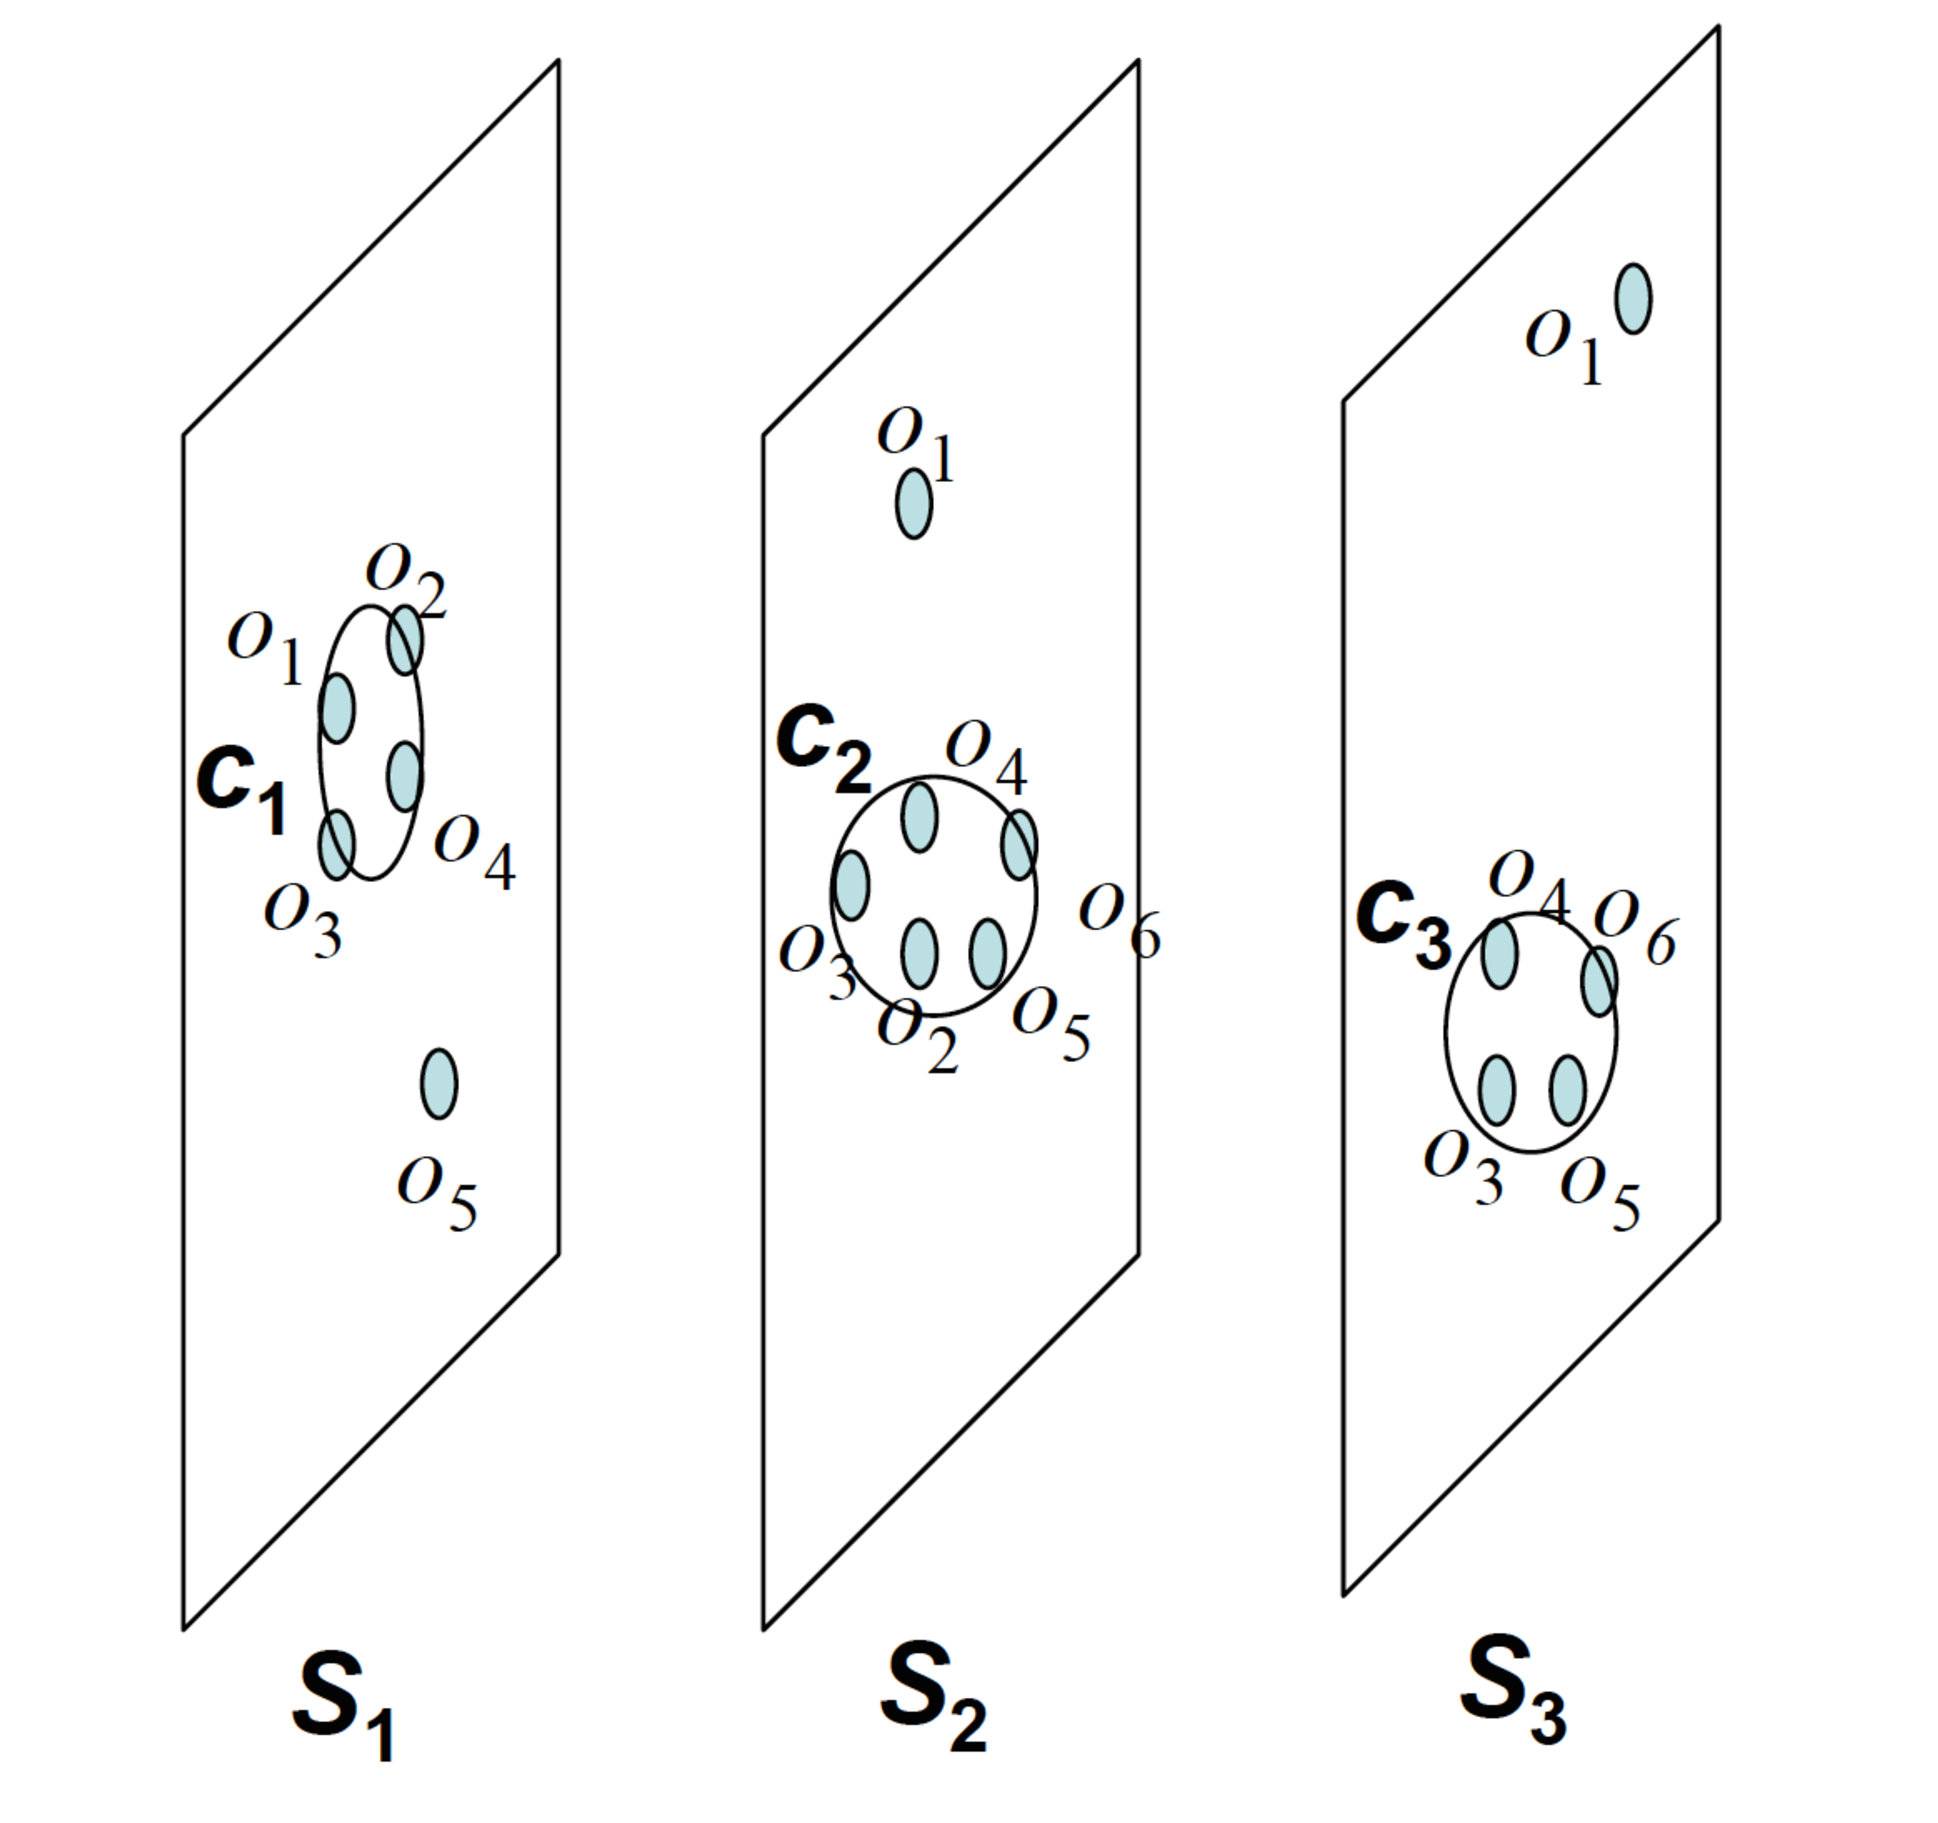
\includegraphics[width=0.5\textwidth]{images/clusters.eps}}
    \footnotesize{Source: \citep{movingclusters}.}
    \label{fig:clusters}
\end{figure}

Jeung et al. proposes the convoy pattern \citep{convoy2}\citep{convoy}. They first point out the key difference between
flock and convoy patterns: flock pattern relies on all trajectories being present in a disk of pre-defined radius, while
convoy does not rely on any kind of shape to cluster its trajectories. That difference is depicted in
\figref{fig:convoy_pattern}, where the second disk is of different size of the other disks and not all trajectories are
present in the consecutive clusters (another difference from the flock pattern). The authors propose three density based
algorithms to find convoy patterns using line simplification techniques. Their work is inspired by the algorithms
already proposed by Kalnis et al. \citep{movingclusters} and \textit{\ac{dbscan}} \citep{dbscan}. More work on convoy
patterns can be found with Aung et al. \citep{convoy3}, where they divide convoy patterns in two different groups,
namely \textit{\acp{dc}} and \textit{\acp{ec}}. To this end, they present three algorithms to identify \ac{ec} patterns.

\begin{figure}
    \centering
    \caption{A Convoy pattern}
    \centerline{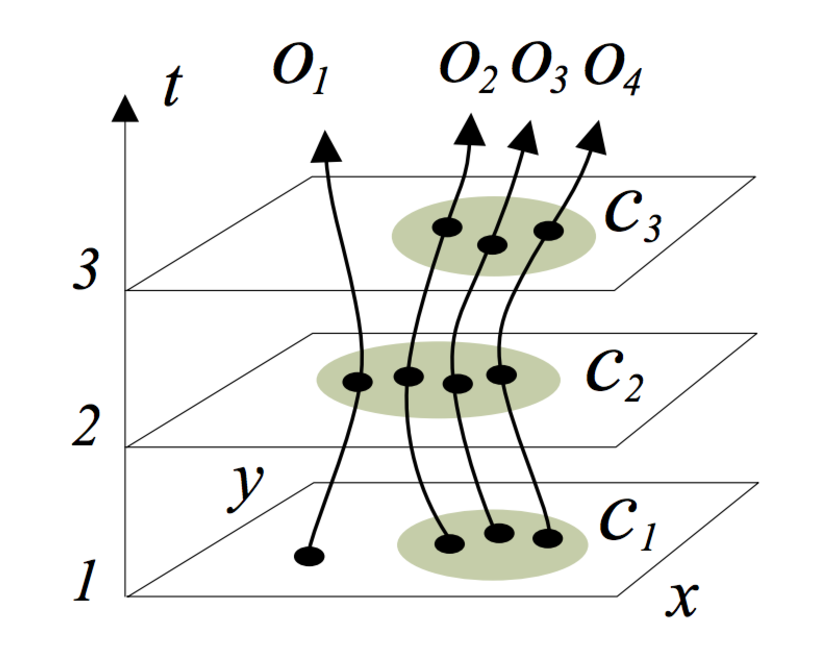
\includegraphics[width=0.5\textwidth]{images/convoy.eps}}
    \footnotesize{Source: \citep{convoy2}.}
    \label{fig:convoy_pattern}
\end{figure}

Gathering is another moving pattern that was analyzed by the academia. Zheng et al. \citep{gathering} state that a
gathering pattern consists in various grouped incidents such as celebrations, parades, protests, traffic jams, etc. They
first formalize and model the gathering pattern and then propose algorithms to find the such pattern. Effectiveness and
efficiency evaluations are presented, showing an overall good result, however only one dataset is analyzed. Instead of
looking for patterns that happen exactly at the same time (e.g. clusters and flocks), Li et al. \citep{swarm} propose
the swarm pattern. Such pattern tries to group \acp{mo} that may actually diverge temporarily and congregate at certain
timestamps, it is not required also that a trajectory stays all the time with the same swarm cluster. The authors in
that work formalize the swarm concept and present algorithms to find the pattern. The effectiveness of the algorithms
is compared against convoy pattern algorithms and it is shown that, for some datasets, the swarm pattern is better
suited.

An algorithm to find patterns in Origin-Destination databases, meaning that only the origin and destination points of a
trajectory are recorded in the analyzed dataset, is presented by Guo et al. \citep{discovering_orig_dest}. They proposed
a way to model points of interest, since \acp{mo} going to the same place (e.g. airport) will report different \ac{gps}
coordinates. The proposed algorithm has a preprocessing phase that makes a Delaunay Triangulation of the points and then
clusters those points based on two parameters: ($k$) the number of points to build a cluster and ($\theta$) the minimum
number of points (or weight) of a cluster. After building the clusters, they derive some mobility measures, in order to
extract spatial and temporal mobility patterns, presenting an useful way of understanding traffic loads in a city.

Baratchi et al. proposed a way to find frequently visited paths between two points of interests. The authors presented
an algorithm that deals with trajectory uncertainty and uses cluster based techniques to map uncertain trajectories to
actual paths in a map that were most likely to be followed by the \ac{mo}. First they gathered points of interests
(those where the \ac{mo} stayed for at least 30 minutes with its speed close to 0) and grouped all subtrajectories that
had the same start and end points of interest. They then applied their algorithm, which consists in dividing the space
in grids and assigning each point to a grid, and partitioned those subtrajectories in even small subtrajectories based
on breakpoints.  After that partition step they used a score mechanism to decide which set of subtrajctories are more
likely to be a frequent path. Their algorithm is mainly targeted for offline analyses and uses a map matching algorithm
in order to match \ac{gps} points to actual map segments. They did not present the dataset used for evaluation nor the
numbers of such dataset. Their evaluation was somewhat shallow and did not present any take away results.

A comprehensive state-of-the-art review in trajectory data mining is presented by Zheng \citep{survey}. He covered
relevant research topics, such as trajectory data preprocessing, trajectory data management, uncertainty of
trajectories, trajectory pattern mining, and trajectory classification. He pointed out some public trajectory datasets
that can be used to evaluate pattern detection algorithms, like the dataset in \citep{tdrive} used in this dissertation.

\section{Flock pattern mining}
\label{sec:rel_flocks}
Gudmundsson et al. \citep{gudefficient} \citep{gudlongest} extended and formalized the flock concept proposed by the
\ac{remo} Framework \citep{remo}. They also introduced the concept that the flock pattern must contain a disk of radius
$R$, enclosing all trajectories, in each time step. They proposed approximation and exact algorithms for flock pattern
detection, but no performance evaluations were made and only theoretical analyses were presented, which does not show if
the algorithms are efficient or not. Later on, the same authors \citep{gudlongest} extended the flock pattern definition
by adding the temporal length variable: the entities must stay together during some time interval $\delta$ to be claimed
as a flock. To this end, they presented some approximation algorithms what work on approximating the radius $R$ of the
disk used to cluster the flock, based on a defined $\epsilon$. The evaluations performed \citep{gudlongest} varied only
the $\delta$ parameter leaving all other parameters variation out of the experiments. Additionally, the performance
results were not good, having scenarios where the algorithms took more than 1500 seconds to analyze a dataset containing
1 million of entries. It is important to say that all algorithms did waste time by analyzing disks that would not form a
flock pattern, thus having a degradation in performance.

Vieira et al. \citep{vieira} proposed a polynomial algorithm to find flock patterns of fixed duration, based in three
parameters: minimum number of trajectories $\mu$, the disk radius $\epsilon$ and a minimum time length $\delta$.  In
order to discover the centers of the cluster disks for each time step, they paired the points that had distance less or
equal to $2*\epsilon$, created two disks based in that pair and tried to cluster other points into those disks. Their
algorithm assumed that each point is sampled in a fixed time interval, assumption that does not reflect real-world
datasets. Additionally, their algorithm suffered from wasting \ac{cpu} cycles by processing disk candidates that were
not real potential flock candidates. The authors also proposed some filtering heuristics to optimize the processing
time, but the optimizations did not present good results, and our local tests showed that the optimizations affected the
final number of flocks found by the algorithm.

An algorithm that mixed together \ac{bfe} \citep{vieira} with a "Frequent Pattern Mining" heuristic is proposed by
Turdukulov et al. \citep{visual}. They made some performance comparison against \ac{bfe} and were able to show some
improvement in the processing time when varying the radius $R$ of the disk. However, despite the improvements, their
results did not propose a fair comparison: (1) \ac{bfe} is an on-line algorithm and their implementation imposed an
offline implementation; (2) they filtered out some trajectories based on random assumptions, e.g. trajectories with less
than 10 minutes or 20 minutes, which might benefit their algorithm and cut out possible flocks of that length; (3) they
only showed results varying the disk radius and not the other parameters used by \ac{bfe}.

The problem of \ac{mfp} is addressed by the work of Geng et al. \citep{enumeration}, which proposed algorithms to
enumerate all \ac{mfp} in a trajectory dataset. \ac{mfp}, in other words, means that the flock cannot be extended
without increasing the disk radius $R$. They proposed a set of algorithms for finding \ac{mfp} and proved that they
could indeed enumerate all \ac{mfp} from a trajectory dataset. They also compared their algorithms with \ac{bfe} from
Vieira et al. \citep{vieira} and showed that their implementations outperformed the later in some scenarios. However,
they still wasted \ac{cpu} cycles by analyzing disks that would be discarded later, by not being potential flock
candidates.

Wachowicz et al. \citep{flockpedestrian} and Wirz et al. \citep{pedestriancanyons} presented algorithms for finding
flocks using pedestrian spatio-temporal data. The former performed a lot pre- and post-processing in the dataset (which
makes not possible to be used in real-time analysis) and neither performance nor accuracy evaluations were presented.
The latter, did not provide any performance evaluation either, only showing accuracy experiments with a tiny dataset of
only 13 entities in a time span of 32 minutes.

Wang et al. \citep{visualtrafficjam} proposed a framework for detecting traffic jams in trajectory data, which can be
considered as a flock pattern, since \acp{mo} stay together in a road during an interval of time. They listed the
requirements for both a data model and a visual interface for their system, in order to be able to expose useful
information for users and extract conclusions from the analysis. Their algorithm was bound to a map network, which means
that one part of data preprocessing would be to map the data points to the respective roads in a map. They claimed to be
able to detect traffic jams with high accuracy, however they did not have any ground truth data to validate the
assumptions. It is also worth noting that only one dataset was used to evaluate the proposed system, which did not show
that the solution was ready for varied data scenarios.

There were also some studies focusing on indoor flock detection using mobile phone sensors, in which Wi-Fi signal
strengths were mapped into coordinates \citep{mobile1}, or a variety of mobile phone sensors (e.g. accelerometer,
magnetometer and Wi-Fi) were used to detect flock patterns \citep{mobile2}. However, those studies only addressed flock
detection in indoor environments, not using \ac{gps} coordinates, which are not in the scope of the problem addressed by
this dissertation.

\section{Academic Contribution}
It is notorious, from the related work presented in \secref{sec:rel_general} and \secref{sec:rel_flocks}, that there is
a lot to cover in order to provide efficient flock pattern detection as well as an elegant and comprehensive system
architecture to the pattern detection problem (which was not seen in any of the presented works). All of that is a
subject to care about due to the extensive number of scenarios that data pattern mining, as well as flock patterns, can
help and be applied to. We can have flock pattern detection helping the following, to name a few \citep{applications}:

\begin{enumerate}
    \item \textbf{Traffic Management}: Unusual grouping of vehicles, or abnormal traffic volume in certain regions can
        be detected with the help of flock pattern detection algorithms. That information can help the accountable
        entities to better plan cities or traffic spaces.
    \item \textbf{Surveillance and Security}: Suspicious movements of groups of people or vehicles can indicate a
        security threat and automatic pattern detection systems can aid the detection of abnormal behavior in a group of
        \acp{mo}.
    \item \textbf{Human Movement}: Governmental organizations can study how people are moving from one part of the
        city/country/state to another with the help of flock pattern detection. They can also acquire information about
        the habits of the population and provide resources to enhance life quality of those involved.
\end{enumerate}

In \secref{sec:architecture} we will propose an elegant and extensible System Architecture that will be able address
pattern detection problems. Such architecture will be divided in logic modules and components, each one with a very
specific and self-contained goal, making then reusable and extensible to address other data analysis problems. We will
also show that by modifying a single component in that architecture will enable the usage of a different software
paradigm, thus proving its modularity, extensibility and ease of use.

We could notice that the presented algorithms suffer from \ac{cpu} cycles waste by processing data that will not
generate any pattern, like the flock disks that contain points that are not present in subsequent time steps. Avoiding
such unnecessary processing can boost the running time of a flock pattern detection algorithm and then provide
information in a real-time fashion for decision takers. With that in mind, we will present an efficient algorithm, based
on bitmaps, that will only be concerned with data that can really generate flock patterns, saving a considerable amount
of time. Moreover, our algorithm will be able to provide information, about the datasets being analyzed, way faster than
other algorithms. We will prove such efficiency by showing benchmarks comparing the running time of our solution against
the state-of-the-art algorithm and also show how that our implementation generates way less unimportant data than the
comparison target algorithm, which dramatically affects the running time of the latter. Last, but not least, we will
provide a multi-core aware implementation of our algorithm, taking advantage of the proposed system architecture
mentioned in the previous paragraph, which will achieve even more savings in running time, without affecting the number
of flocks that are found.  Aiming at showing that our solution is ready for multiple types of data, we will perform
experiments with 4 different datasets, being them real and synthetic generated and with a large amount of data entries,
with some of them having more then 50 million records.

\chapter{Technical Background}
\label{chp:techbackground}

We now present some technical background that will be required to understand the remaining of this dissertation.

\section{Trajectory and data information}
\label{sec:tech_data}

Spatio-temporal datasets usually come in the form of a set of tuples $\{O_{id}, \phi, \lambda, t\}$. Where: $O_{id}$
uniquely identifies a Moving Object (MO); $t$ corresponds to the time stamp that the GPS position was extracted; $\phi$
and $\lambda$ corresponds to the latitude and longitude of the MO respectively, at a given time stamp $t$. Each MO
represented by a $O_{id}$ has a trajectory $T_{id}$ associated with it, being a trajectory defined as follows.

\begin{Def}
Given an $O_{id}$, an trajectory $T_{id}$ consists of a sequence of 3-D points, belonging to $O_{id}$ in the form of
$<(\phi_0, \lambda_0, t_0), (\phi_1, \lambda_1, t_1), ..., (\phi_n, \lambda_n, t_n)>$, with $n \in \mathbb{N}$ and $t_0
< t_1 < ... < t_n$.
\end{Def}

GPS coordinates are often represented using the World Geodetic System 1984 (WGS84) \citep{wgs84}, which can make some
mathematical operations needed by the algorithm proposed in this dissertation (e.g. vectorial operations) harder to be
performed. Given that limitation, once coordinates are read from a database, transformations from WGS84 to the
$\mathbb{R}^2$ system are made. We use $0^\circ$ as both latitude and longitude coordinates for our origin point in the
$\mathbb{R}^2$ system and execute the algorithm used by the Woods Hole Oceanographic Institution (WHOI) to perform the
conversion from WGS84 to $\mathbb{R}^2$ on the fly \citep{latlogtoxy}.

It is worth noting that real world datasets do not guarantee that all points of all trajectories are sampled in the same
rate. In a ideal world, a perfect spatio-temporal dataset would have entries as described in \tabref{tbl:ideal_rate},
where one can see that each $O_{id}$ has its position sampled in intervals of 1 $t$ unit. However, that is not what
happens in real world datasets. \tabref{tbl:real_rate} presents how MOs have their position sampled over time: no fixed
rate interval due to transmission noises, precision issues and other problems that can make the sample rate varying a
lot from $O_{id}$ to $O_{id}$. Therefore, we need to have a way to be able to compare and group points belong to the
same logical time interval. With that in mind, we divided the time extent in buckets of size $\sigma$ where $\sigma$
should be chosen accordingly to the dataset being analyzed, based on the sampling rate of points. Hence, from this point
forward, every time when we refer to any time instance $t_i$ we are actually talking about the $i_{th}$ time bucket (or
time slot) of size $\sigma$.

\begin{table}
    \centering
    \begin{minipage}{0.5\textwidth}
        \centering
        \caption{Ideal dataset sample rate}
        \label{tbl:ideal_rate}
        \begin{tabular}{c c c c}
            \toprule
            \textbf{$O_{id}$} & \textbf{$\phi$} & \textbf{$\lambda$} & \textbf{$t$} \\
            \toprule
            0 & 38.018470 & 23.845089 & 0 \\
            1 & 38.018069 & 23.845179 & 0 \\
            2 & 38.018241 & 23.845530 & 0 \\
            3 & 38.017440 & 23.845499 & 0 \\
            4 & 38.015609 & 23.844780 & 0 \\
            \bottomrule
            0 & 38.015609 & 23.844780 & 1 \\
            1 & 38.014018 & 23.844780 & 1 \\
            2 & 38.012569 & 23.844869 & 1 \\
            3 & 38.011600 & 23.845360 & 1 \\
            4 & 38.010650 & 23.845550 & 1 \\
            \bottomrule
            0 & 38.010478 & 23.845100 & 2 \\
            1 & 38.010478 & 23.845100 & 2 \\
            2 & 38.010508 & 23.844640 & 2 \\
            3 & 38.010520 & 23.844530 & 2 \\
            4 & 38.010520 & 23.844530 & 2 \\
            \bottomrule
        \end{tabular}
    \end{minipage}%
    \hfill
    \begin{minipage}{0.5\textwidth}
        \centering
        \caption{Real world dataset sample rate}
        \label{tbl:real_rate}
        \begin{tabular}{c c c c}
            \toprule
            \textbf{$O_{id}$} & \textbf{$\phi$} & \textbf{$\lambda$} & \textbf{$t$} \\
            \toprule
            0 & 38.018470 & 23.845089 & 4 \\
            1 & 38.018069 & 23.845179 & 0 \\
            2 & 38.018241 & 23.845530 & 1 \\
            3 & 38.017440 & 23.845499 & 10 \\
            4 & 38.015609 & 23.844780 & 8 \\
            \bottomrule
            0 & 38.015609 & 23.844780 & 6 \\
            1 & 38.014018 & 23.844780 & 5 \\
            2 & 38.012569 & 23.844869 & 2 \\
            3 & 38.011600 & 23.845360 & 16 \\
            4 & 38.010650 & 23.845550 & 12 \\
            \bottomrule
            0 & 38.010478 & 23.845100 & 14 \\
            1 & 38.010478 & 23.845100 & 6 \\
            2 & 38.010508 & 23.844640 & 3 \\
            3 & 38.010520 & 23.844530 & 25 \\
            4 & 38.010520 & 23.844530 & 30 \\
            \bottomrule
        \end{tabular}
    \end{minipage}
\end{table}

\begin{table}[h!]
    \centering
    \caption{Mapping points from \tabref{tbl:real_rate} to its correspondent time slot, using $\sigma = 3$}
    \label{tbl:timeslot}
    \begin{tabular}{c c c c c}
        \toprule
        \textbf{$O_{id}$} & \textbf{$\phi$} & \textbf{$\lambda$} & \textbf{$t$} & \textbf{Time slot} \\
        \toprule
        0 & 38.018470 & 23.845089 & 4 & 1 \\
        1 & 38.018069 & 23.845179 & 0 & 0 \\
        2 & 38.018241 & 23.845530 & 1 & 0 \\
        3 & 38.017440 & 23.845499 & 10 & 3 \\
        4 & 38.015609 & 23.844780 & 8  & 2 \\
        \bottomrule
        0 & 38.015609 & 23.844780 & 6 & 2 \\
        1 & 38.014018 & 23.844780 & 5 & 1 \\
        2 & 38.012569 & 23.844869 & 2 & 0 \\
        3 & 38.011600 & 23.845360 & 16 & 5 \\
        4 & 38.010650 & 23.845550 & 12 & 4 \\
        \bottomrule
        0 & 38.010478 & 23.845100 & 14 & 4 \\
        1 & 38.010478 & 23.845100 & 6 & 2 \\
        2 & 38.010508 & 23.844640 & 3 & 1 \\
        3 & 38.010520 & 23.844530 & 25 & 8 \\
        4 & 38.010520 & 23.844530 & 30 & 10 \\
        \bottomrule
    \end{tabular}
\end{table}

\tabref{tbl:timeslot} shows in which time slot each $O_{id}$ entry will end up at. The assignment of the time slot is
made by dividing the timestamp value by the bucket size $\sigma$ and then performing a floor operation, as shown in
\eqnref{eq:timeslot}.

\begin{equation}
    \label{eq:timeslot}
    s = \floor*{\frac{t}{\sigma}}
\end{equation}

\section{Flock pattern}
\label{sec:tech_flock}
We use the same definition of flock from Vieira et al. \citep{vieira}:

\begin{Def}
\label{def:flock}
Given a set of trajectories $\mathcal{T}$, a minimum number of trajectories $\mu > 1$ ($\mu \in \mathbb{N}$), a maximum
distance $\epsilon > 0$ defined over the distance function $d$, and a minimum time duration $\delta > 1$ ($\delta \in
\mathbb{N}$). A flock pattern $Flock (\mu, \epsilon, \delta)$ reports all maximal size collections $\mathcal{F}$ of
trajectories where: for each $f_k$ in $\mathcal{F}$, the number of trajectories in $f_k$ is greater or equal than $\mu$
($|f_k| \ge \mu$) and there exist $\delta$ consecutive time stamps such that for every $t_i \in [f_k^{t_1}...f_k^{t_1 +
\delta}]$, there is a disk with center $c_k^{t_i}$ and radius $\epsilon/2$ covering all points in $f_k^{t_i}$. That is:
$\forall f_k \in \mathcal{F}, \forall t_i \in [f_k^{t_1}...f_k^{t_1 + \delta}], \forall T_j \in f_k: |f_k | \ge \mu,
d(p_j^{t_i},c_k^{t_i}) \le \epsilon/2$.
\end{Def}

\begin{figure}[h!]
    \centering
    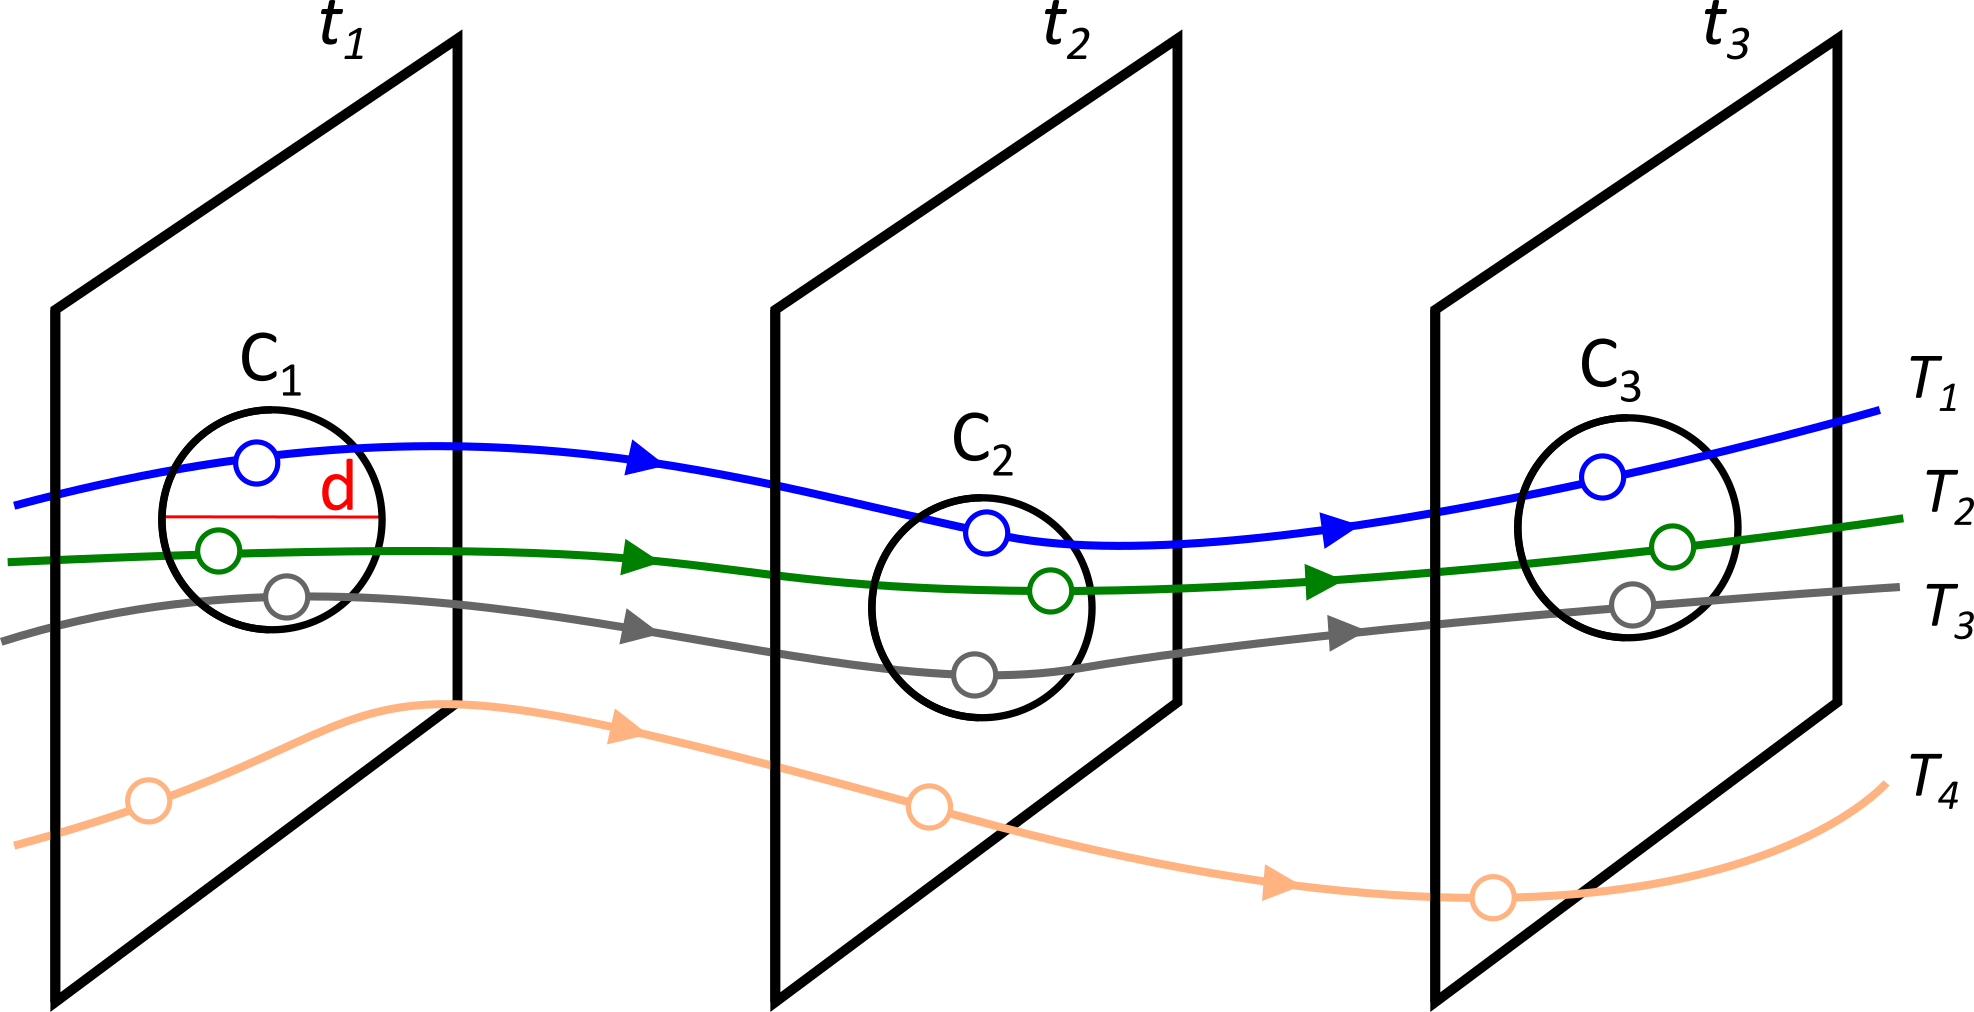
\includegraphics[width=\textwidth]{images/flock_2.png}
    \caption{T1, T2 and T3 form a flock of size 3 with minimum length of three time slots, with a disk enclosing all
        trajectories at each time slot}
    \label{fig:flock2}
\end{figure}

In other words, what \defref{def:flock} states is that a flock pattern basically consists in a set of at least $\mu$
trajectories (where each trajectory $T_{id}$ belongs the MO represented by $O_{id}$) that stay together for a minimum
time extent $\delta$.  Additionally, in order to be considered a flock, there must exist a disk, with radius
$\epsilon/2$, that encloses all points of all trajectories for each time slot. Hence, we have a Flock pattern relying on
three key parameters:
\begin{enumerate}
    \item $\mu$: the minimum number of trajectories, in order to be considered a flock
    \item $\epsilon$: diameter of the disk that needs to enclose the trajectories for each time slot
    \item $\delta$: the minimum number of time slot units that the trajectories need to stay together
\end{enumerate}

This definition is well depicted in \figref{fig:flock2}, where you can see for each time slot $t_i$ it exists a disk of
diameter $\epsilon = d$ enclosing the points of trajectories $T_1$, $T_2$ and $T_3$. Hence, if we have set our flock
parameters to $\mu = 3$, $\epsilon = d$ and $\delta = 3$, we would have found the flock pattern $f = \{T_1, T_2, T_3\}$
shown in \figref{fig:flock2}. It is worth noting that trajectory $T_4$ could not be part of the flock pattern because it
was not possible to find a disk of diameter $d$ that would enclose 2 more trajectories with $T_4$ in each time slot
$t_i$.

\subsection{Disk discovery}
\label{subsec:disk_discovery}

One of the most important part that enables the flock pattern identification is how to efficiently discover the disks
that can enclose potential flock patterns. Since the disk does not need to have its center in any of the points in the
dataset, there can be infinite places to look for disk in the dataset space. Vieira et al. \citep{vieira} propose a way
to reduce that search space to a finite number of locations, which we will explain in the remaining of this section and
will be used in the work proposed in this dissertation.

\begin{figure}[h!]
    \centering
    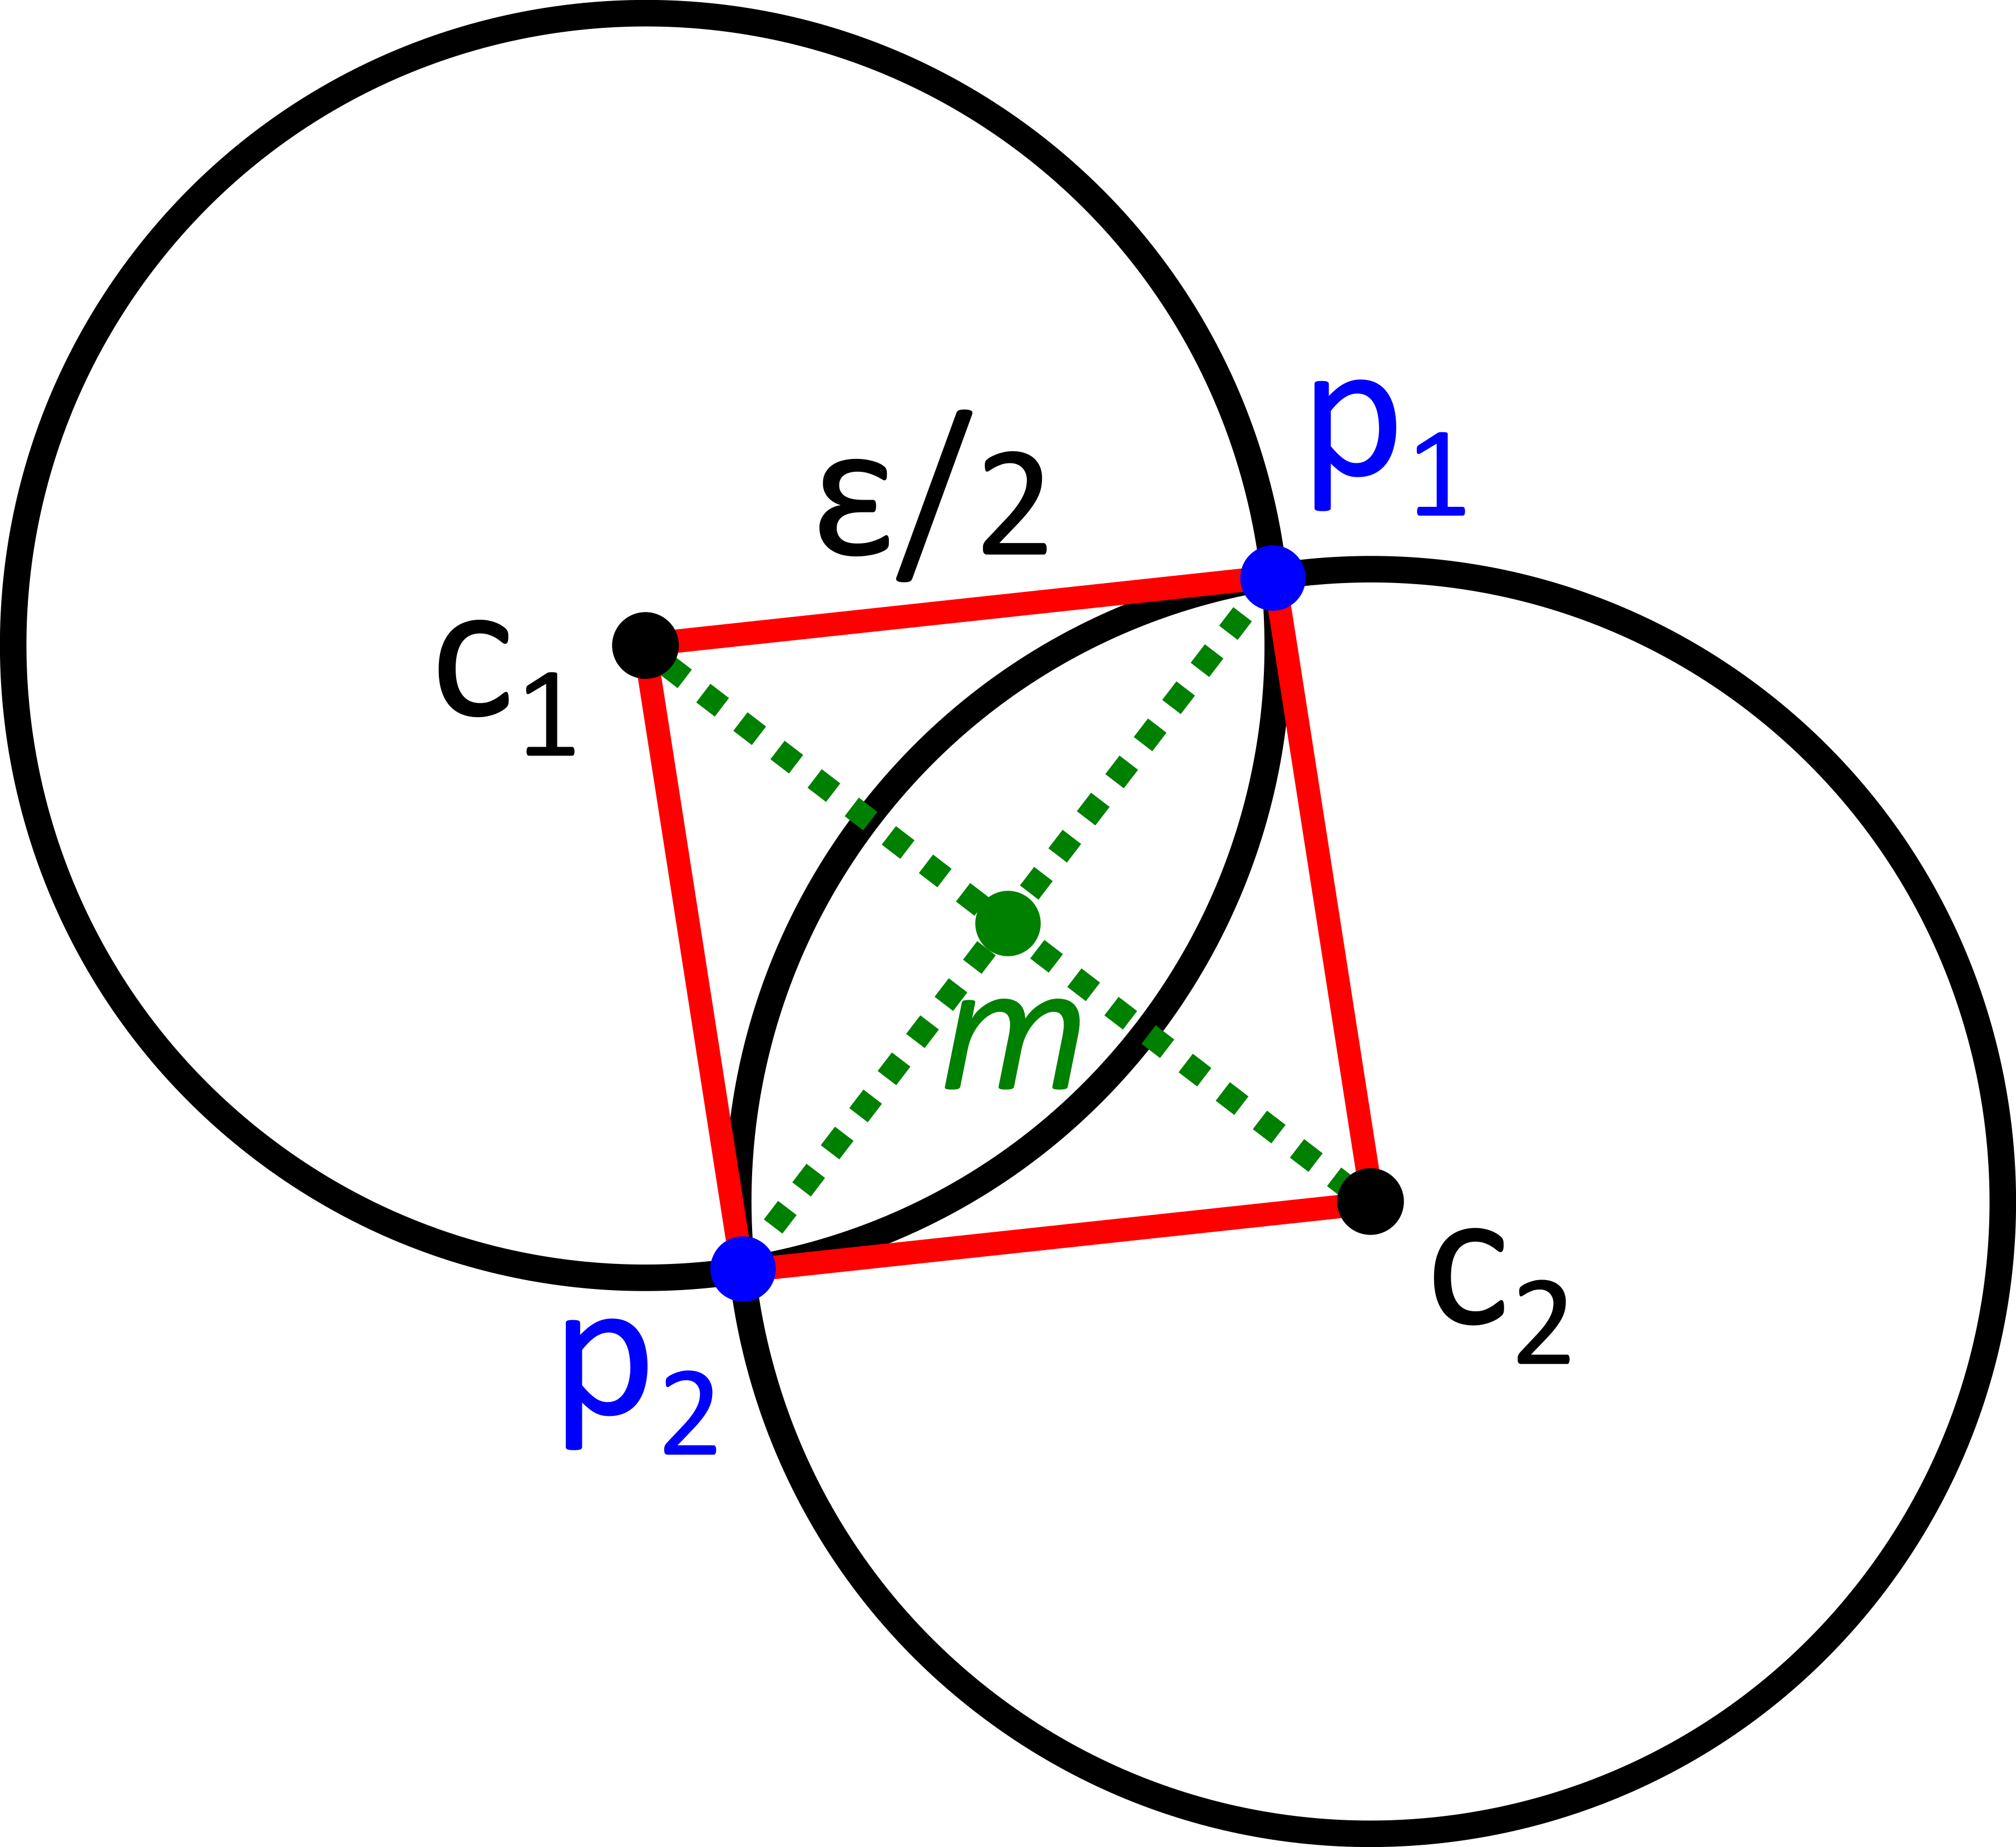
\includegraphics[width=0.7\textwidth]{images/disks_discovery.png}
    \caption{Two disks with radius $\epsilon/2$ that are found based on points $p_1$ and $p_2$. $c_1$ and $c_2$ stands
        for the disks centers and $m$ represents the midpoint of $p_1$ and $p_2$.}
    \label{fig:disks_discovery}
\end{figure}

We can easily find two circles that intersect two points using some vectorial operations as shown in
Algorithm~\ref{alg:disks} below.

Given two GPS points $p_1$ and $p_2$, we get the values of $x1$ and $y1$, which will correspond to the longitude and
latitude in meters (such conversion is mentioned in \secref{sec:tech_data}) of $p_1$, and $x2$ and $y2$ being the
equivalent of $p_2$ (lines 1 to 4). We know that the centers of the two disks $c_1$ and $c_2$ that can be generated by
those two points, lie in the line that is orthogonal to points $p_1$ and $p_2$ and passes through the midpoint $mid$ of
those same points. After calculating $mid$ (lines 6 and 7) we convert those same points into a vector $v$ (lines 9 and
10) and take its length (line 12), which will be used later to normalize $v$. Line 13 calculates the distance $c_d$ the
centers are from the $mid$ whereas lines 15 and 16 calculates the orthogonal vector $o$ for $v$, which will guide the
direction for the disks centers. The algorithm ends by find the centers of the disks $c_1$ and $c_2$ by adding and
subtracting the multiplication of normalized $o$ by $c_d$ to $mid$. The circles that we can find are well depicted in
\figref{fig:disks_discovery}.

\begin{algorithm}
\caption{Disks Discovery}
\label{alg:disks}
\begin{algorithmic}[1]
    \State $x1 \gets p1.longitudeMeters$
    \State $y1 \gets p1.latitudeMeters$
    \State $x2 \gets p2.longitudeMeters$
    \State $y2 \gets p2.latitudeMeters$
    \State
    \State $midX \gets \frac{x1 + x2}{2}$
    \State $midY \gets \frac{y1 + y2}{2}$
    \State
    \State $vectorX \gets x2 - x1$
    \State $vectorY \gets y2 - y1$
    \State
    \State $pointsDistance \gets \sqrt{vectorX^2 + vectorY^2}$
    \State $centerDistFromMidPoint \gets \sqrt{(\frac{\epsilon}{2})^2 - (\frac{pointsDistance}{2})^2}$
    \State
    \State $orthogonalVectorX \gets vectorY$
    \State $orthogonalVectorY \gets -vectorX$
    \State
    \State $normalizedOrtVectorX \gets \frac{orthogonalVectorX}{pointsDistance}$
    \State $normalizedOrtVectorY \gets \frac{orthogonalVectorY}{pointsDistance}$
    \State
    \State $c1X \gets midX + (centerDistFromMidPoint * normalizedOrtVectorX)$
    \State $c1Y \gets midY + (centerDistFromMidPoint * normalizedOrtVectorY)$
    \State
    \State $c2X \gets midX - (centerDistFromMidPoint * normalizedOrtVectorX)$
    \State $c2Y \gets midY - (centerDistFromMidPoint * normalizedOrtVectorY)$
\end{algorithmic}
\end{algorithm}

In order to avoid running Algorithm~\ref{alg:disks} through all the points found in a time slot $t_i$, Vieira et al.
\citep{vieira} proposed a grid structure to reduce the search space for the set of points. In that approach, all points
that belong to time slot $t_i$ will be arranged into a grid with cells of size $\epsilon$. After that, we will go
through each cell $g_{i,j}$ in the grid and perform a search for points that are at most $\epsilon$ distant from each
other. That search can be restricted to the cells $g_{i - 1, j - 1} ... g_{i + 1, j + 1}$, as depicted in
\figref{fig:grid}, because all cells have $\epsilon$ as their size. It is important to note that the size of $\epsilon$
directly impacts in the number of cells and the number of points in each cell. For example, for a very small $\epsilon$
more cells will be created and less points will be present in each cell.  O the other hand, large $\epsilon$ will create
less but more populated cells.

\begin{figure}[h!]
    \centering
    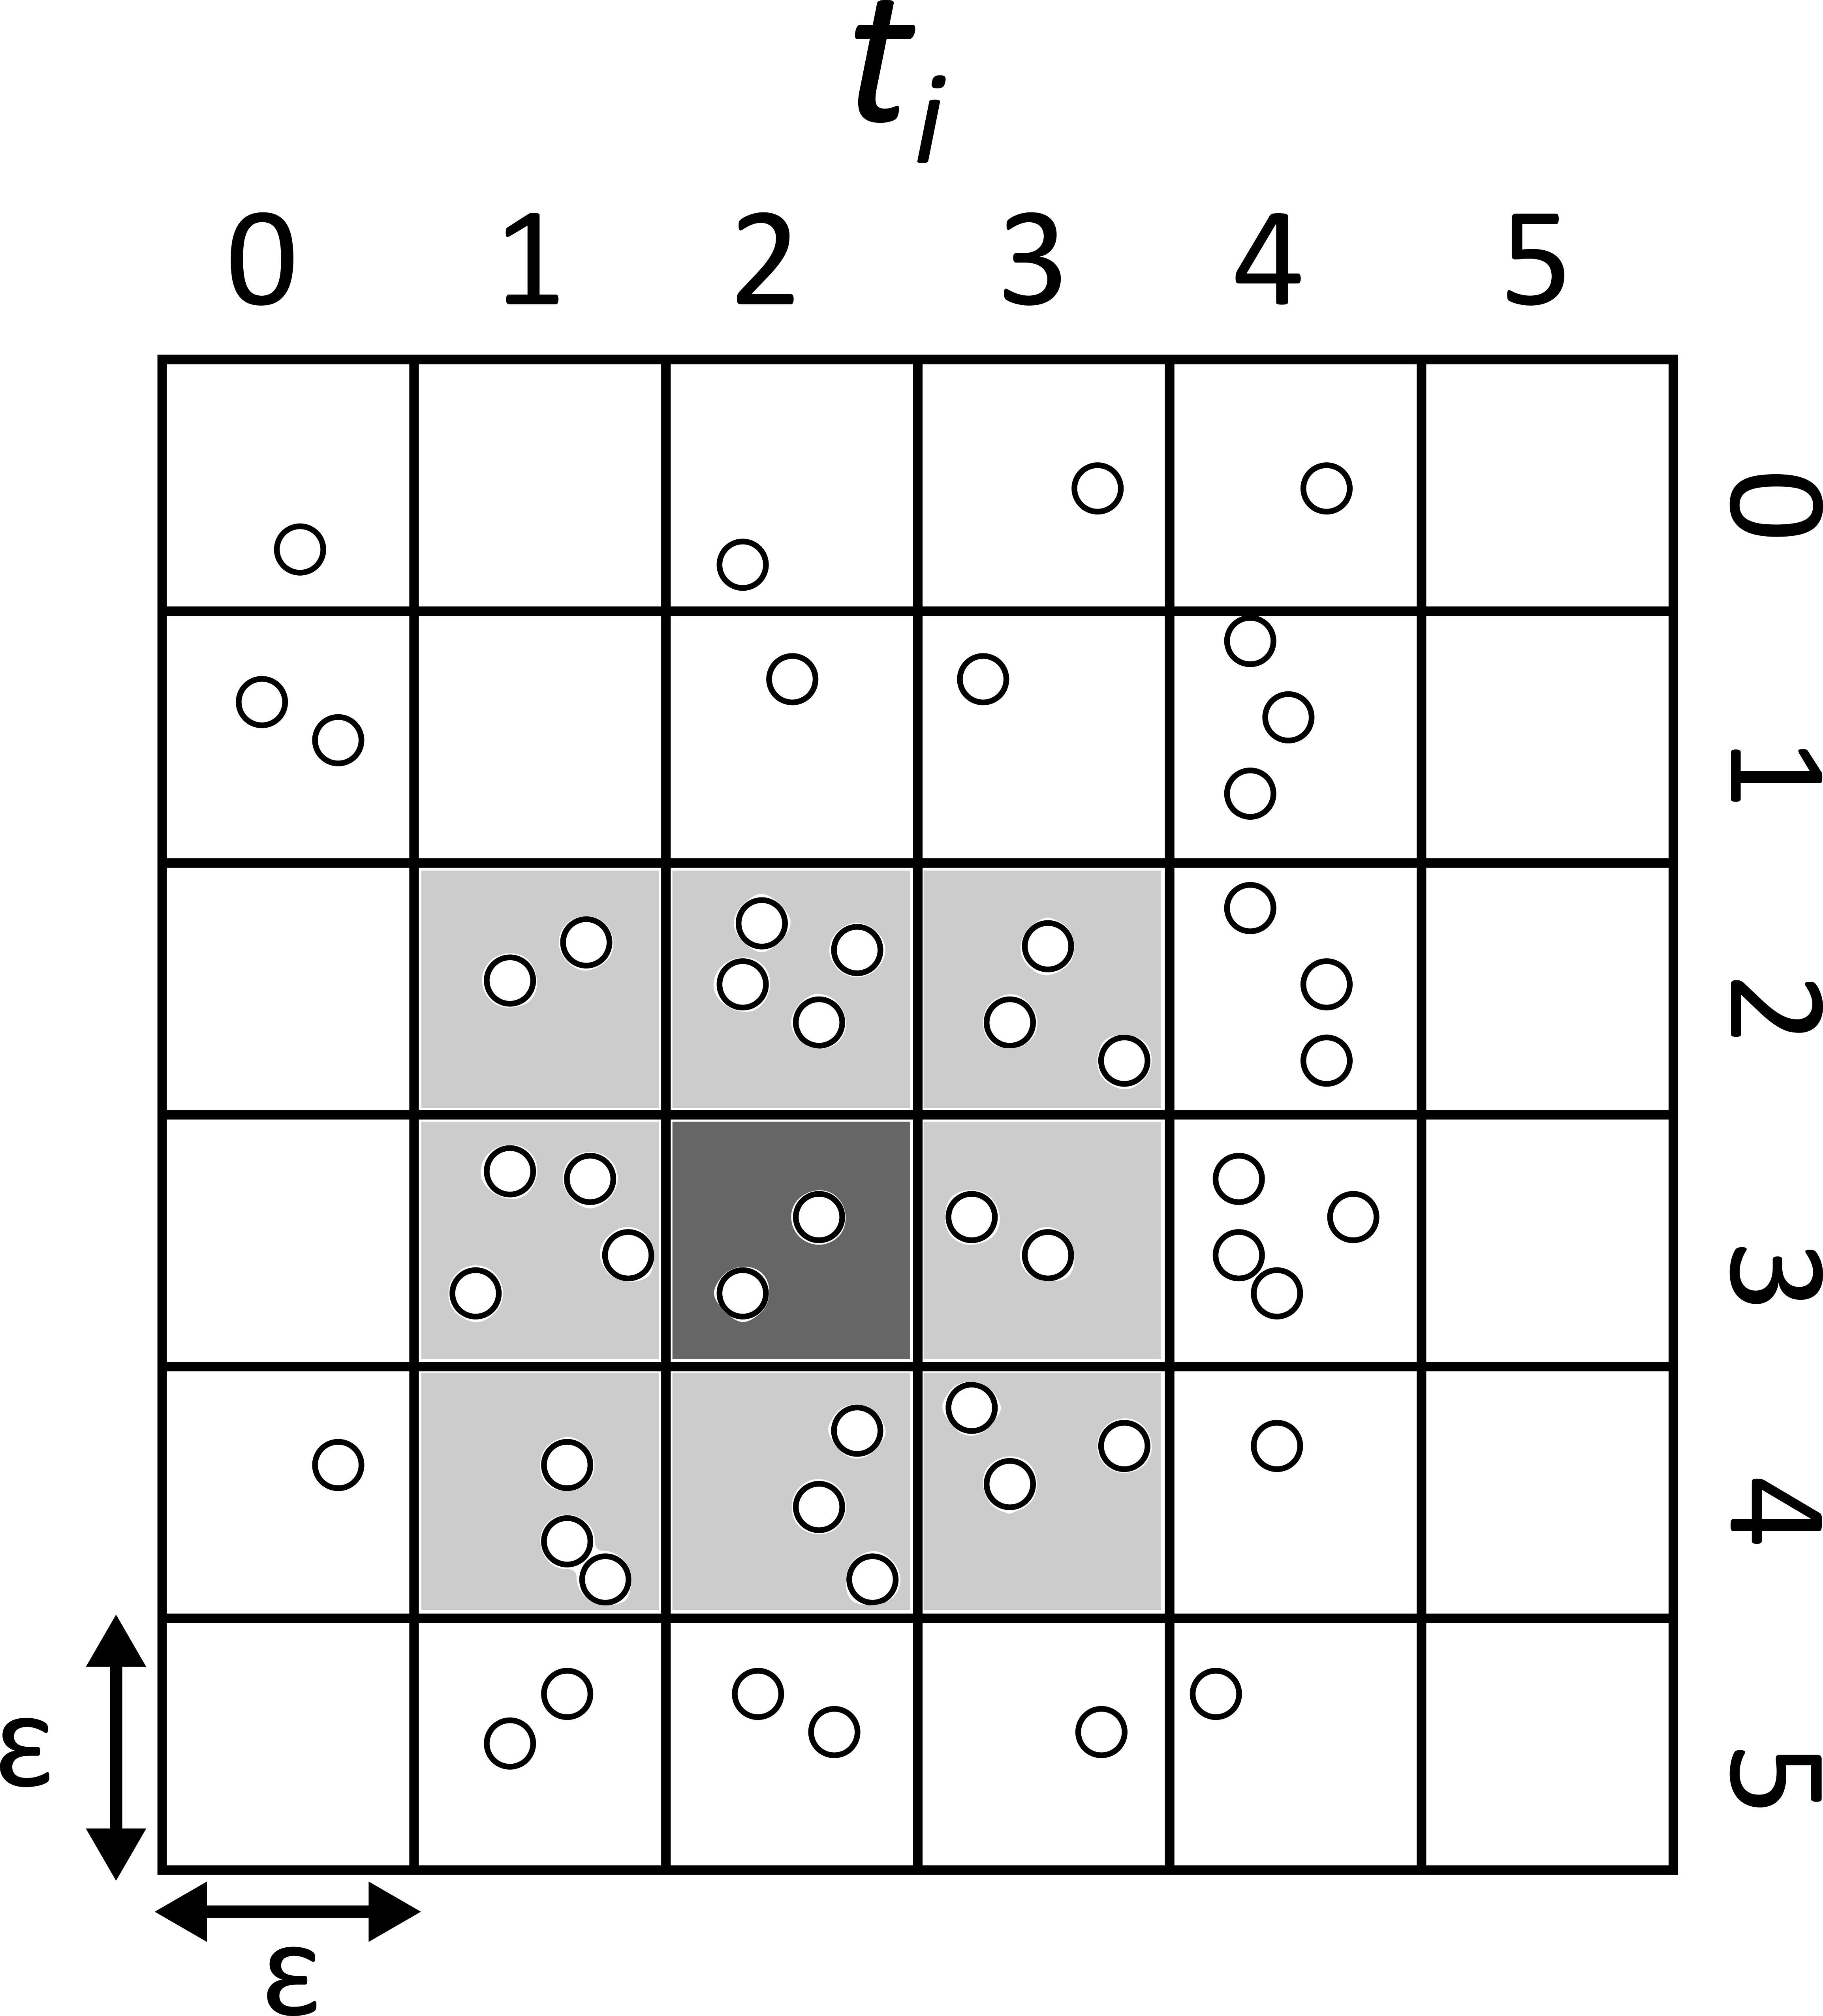
\includegraphics[width=0.7\textwidth]{images/grid.png}
    \caption{Point grid for time slot $t_i$. The dark grey is the grid that is currently being processed and the light
        grey grids around, are the grids that will be in the search space of the dark grid. Each small circle inside the
        grid, represents a GPS point that was collected in time slot $t_i$}
    \label{fig:grid}
\end{figure}

Algorithm~\ref{alg:grid} shows how we will construct the grid structure for a set of points from a specific time slot
$t_i$. In order to represent a grid structure, we will use a map of indexes to a list of points, which will then be
populated as follows. For each point $p$ in the point set, we will \textit{bucketize} the longitude and the latitude of
the point (both converted to meters, using \eqnref{eq:timeslot}) by dividing them by the cell size $\epsilon$ (lines 5
and 6).  Once we have the division results, we will convert them to string and concatenate them, forming a cell index
(line 8).  With the cell index in hand, we need only to add the point to the corresponding cell (line 9). It is worth
noting that this proposed approach will not create empty cells, saving memory and unnecessary processing time.

\begin{algorithm}
\caption{Construct Grid}
\label{alg:grid}
\begin{algorithmic}[1]
    \State $grid \gets map\{index, [...]\}$ \Comment map of cell index to list of points that belong to that cell
    \State $points \gets \Call{GetPointsOfTimeSlot}{t_i}$
    \State
    \For{each point $p$ in $points$}
        \State $xIndex \gets \floor*{\frac{p.longitudeMeters}{\epsilon}}$
        \State $yIndex \gets \floor*{\frac{p.latitudeMeters}{\epsilon}}$
        \State
        \State $index \gets \Call{ToString}{xIndex} + "\_" + \Call{ToString}{yIndex}$
        \State $grid[index].add(p)$
    \EndFor
\end{algorithmic}
\end{algorithm}

Another important concept to keep in mind is that we are only interested in the maximum disks. Once we have found the
disks with the points that belong to them, we will check if any disk $d_i$ is a subset of another disk $d_j$. By saying
that $d_i$ is a subset of $d_j$ we mean that $d_j$ has all the points that $d_i$ has. This was identified as being a
tremendous processing bottleneck for an algorithm that aims at finding flock patterns.

\chapter{Modular and efficient Flock Pattern identification}
\label{chp:solution}
\section{Generic System Architecture}
\label{sec:architecture}
After the related work research that was performed, we noticed a lack of system architecture in order to solve data
spatio-temporal pattern detection problems. So far, no previous work has provide an architecture that could be easily
extensible and reusable for the myriad of the spatio-temporal pattern detection problems in the academy.

We first tried to approach this problem in a more generic fashion, since all moving pattern mining problem has the same
workflow:

\begin{enumerate}
    \item Connect to a spatio-temporal data source
    \item Retrieve and aggregate spatio-temporal data
    \item Process and mine that data in order to find the desired pattern or extract the desired information
\end{enumerate}

With that in mind, we designed a modular and easily extensible architecture that can fit for almost all spatio-temporal
data mining problem, which is depicted by \figref{fig:architecture}. One can notice that we focus on 4 key building
blocks, that can be easily registered/unregistered according to the targeting problem: (1) Data Source Connectors; (2)
Data Decoders; (3) Data Listeners (Data aggregators); (4) Data Processor.

In layer (1) we are concerned on how to retrieve the data, meaning how to communicate properly to the data source in
order to be able to extract each record of spatio-temporal data that the data source can provide. Thus, each "Data
Source Connector" (DSC) depicted in the \textit{Data Connectors' Module} in \figref{fig:architecture} represents a
logical piece that knows how to connect to and extract data from a specific data source. We can have a DSC that knows
how to connect to a MySQL database, or another one that can connect to a cloud based storage system like AWS DynamoDB,
or even a DSC that simply connects to an online data stream and listen for incoming data.

\begin{figure}[h!]
    \centering
    \caption{Generic System Architecture overview}
    \includegraphics[width=\linewidth]{images/architecture.png}
    \label{fig:architecture}
\end{figure}

After connecting and retrieving data from a data source, we need to clean, decode and translate the incoming raw data to
a format that is simple and understandable to our system. To achieve that we will have a Data Decoder (DD) component,
which knows how to interpret the raw data format that comes from a DSC and translate it to a format that layer 3 can
understand. We can see in \figref{fig:architecture} that a DD can register itself to a DSC in order to receive each data
record that a DSC gathers from a data source. It is important to note that a DD can register to only one DSC, but a DSC
can have multiple DD registered to it.

In any problem of data mining, aggregation is one of the most important phases, since it is there that the data
gathering happens and necessary arrangements are made in order to get the data ready for processing. In our system that
is represented by layer (4), which we call the Data Listeners' Module. We can have multiple types of Data Listeners (DL)
in that module, and each of them can perform different types of aggregation and pre-processing depending on the final
goal.  For example, we could have an aggregator that bucketize the GPS points by their timestamp and filter out
outliers, before sending to processing, or another one that performs point interpolation in order to reduce trajectory
uncertainty. Similarly to the DD module, we can a DL can only register to one DD, but a DD can have multiple DL
registered to it. Later on we will see a DL proposed as one of the contributions by this dissertation, which will
perform a \textit{bufferized} aggregation of points.

The last, but not least, remaining piece is the Data Processors' Module, in layer (5). Is there that we will have the
intelligence to perform a data mining task that will generate insights for decision making, detect moving patterns and
the forth. We can have a Data Processor (DP) that detects flock patterns, other that detects convergence patterns and
other that provide traffic information in real time, to name a few. Following the pattern of the aforementioned modules,
each DP can only register to a single DL, but a DL can have multiple DPs registered to it. This dissertation will
present a novel DP for detecting flock patterns, based on the BFE algorithm proposed by Vieira et al. \citep{vieira}.

Researchers and data analysts can leverage from the proposed architecture in order to tackle multiple problems at once,
reusing components that can serve other spatio-temporal pattern mining problems.

\section{Aggregation and data processing efficiency}
\label{sec:bitdf}
By analyzing some of the algorithms proposed in \secref{sec:rel_flocks} and their respective running times, we noticed
that most of the CPU cycles were spent by analyzing disks that will not generate flock patterns, due to the points not
being present in $\delta$ consecutive time slots. In all algorithms, disks generated in time slot $t_{i+1}$ are compared
with those generated in $t_{i}$ in order to check if an extension to a potential flock pattern is found. This operation
has $O(nm)$ complexity, with $n$ being the number of disks and $m$ the number of potential flocks from previous time
slots.  Additionally, for each comparison between a disk and a potential flock, an intersection operation between them
needs to be made.

Things get even worse in algorithms like BFE, where a new created disk $D$ is checked if it is either subset or a
duplicate of a previously found disk (as already mentioned in \secref{subsec:disk_discovery}). The running time of this
step can result in a $O(n^2)$ time complexity in the worst case (with $n$ being the number of disks generated by that
time slot) requiring an intersection operation between each pair of disks that are being compared. We can reduce
significantly that number of disks by only creating disks with points that can potentially form a flock, i.e. with
points that appears in the dataset for $\delta$ consecutive time slots. We measured the time spent in those disk related
operations, using the datasets that we will use in our experiments, and showed the results in
\figref{fig:time_consumption}. There we can see that the disk and flock related operations can reach 99\% of the overall
processing time of the algorithm.

Consider the example depicted in Fig. \ref{fig:disks}, where we are looking for flocks with $\mu=4$ and $\delta=4$. As
we can see, in time slot $t_0$ our dataset reported points $p_1,p_2,p_3$ and $p_4$ and, due to the proximity between
them, disk $d_0$ was created enclosing all four points. In $t_1$ the same points were reported and again the regular
algorithm was able to create another disk $d_1$. However, in $t_2$, $p_3$ was not present and the disk $d_2$ only
contained three points, which is not enough to represent a flock pattern because the number of trajectories is less than
$\mu = 4$. Hence, we could avoid the creation of disks $d_0$ and $d_1$ if we would know in advance that $p_3$ was
missing in $t_2$, saving CPU cycles of disk comparisons in $t_0$ and $t_1$. We argue that when scaled to a dataset of
millions of records with real-time processing, that disk check for subsets and flock extension, in the regular
algorithms, will lead to severe degradation in performance. With that in mind, we can say with high confidence that
reducing the processing time spent with unnecessary disks that won't generate flock patterns, can dramatically reduce
the overall processing time of the algorithm.

\begin{figure}[h!]
    \centering
    \caption{Percentage of time spent between disk and flock processing tasks against other tasks in the algorithm}
    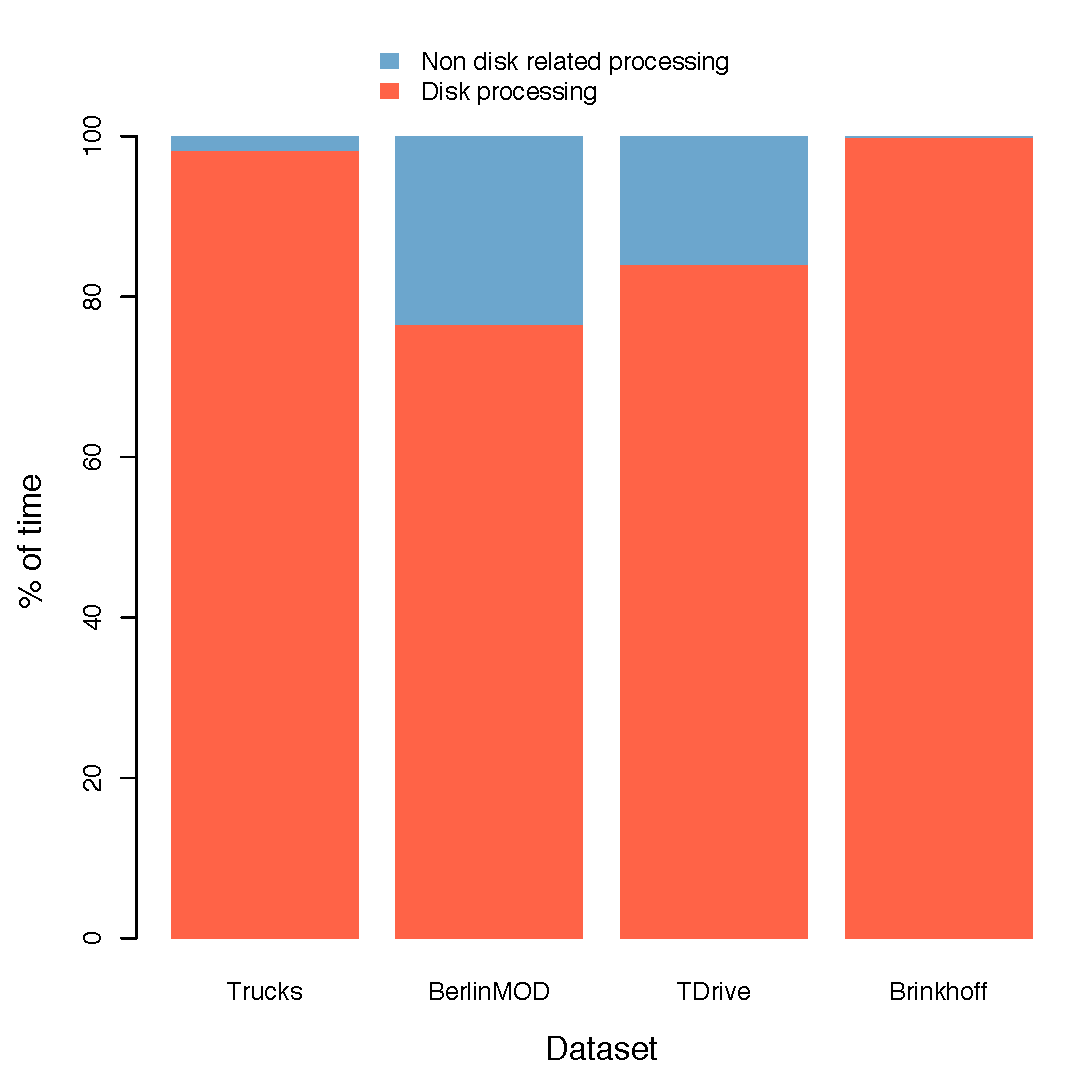
\includegraphics[width=0.7\linewidth]{images/timeConsumption.eps}
    \label{fig:time_consumption}
\end{figure}

\begin{figure}[h!]
    \centering
    \caption{Sequence of disks in 4 consecutive time slots and the points that were clustered to them}
    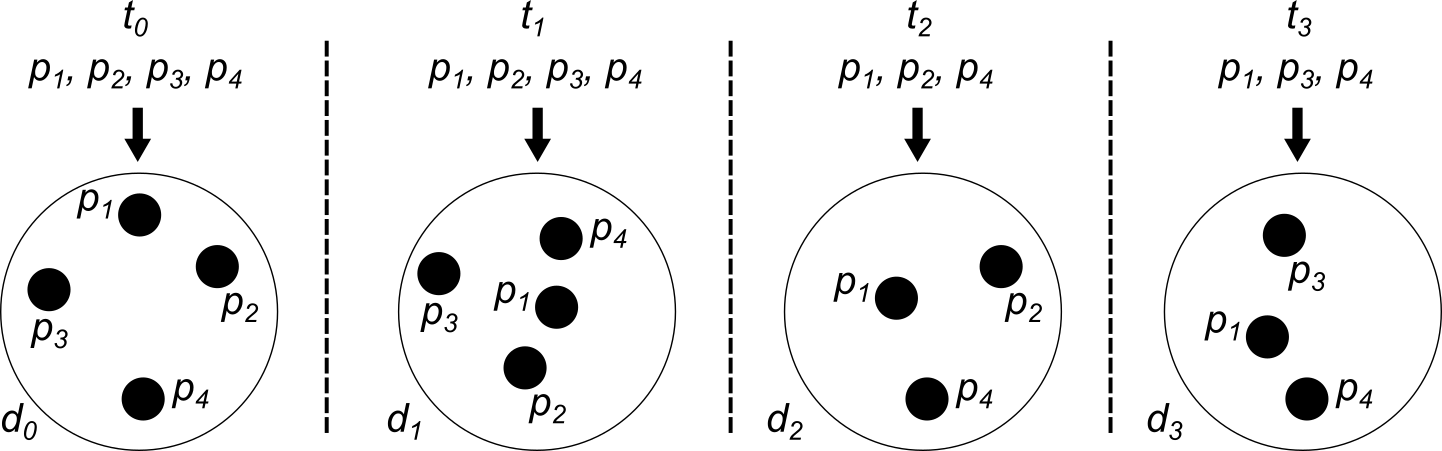
\includegraphics[width=\linewidth]{images/disks_2.png}
    \label{fig:disks}
\end{figure}

\begin{algorithm}[h!]
\caption{GPS Stream Buffering}
\label{alg:gpsb}
\begin{algorithmic}[1]
    \State $pointBuffer \gets map\{index, \{id, point[...]\}\}$
    \State $presenceMap \gets map\{id, bitmap\}$
    \State $lastTimeslot \gets -1$
    \State
    \Procedure{AddPointPresence}{$id$}
        \State $mask \gets \Call{ShiftLeft}{1, pointBuffer.size - 1}$
        \State $presence \gets \Call{BitOr}{presenceMap[id], mask}$
        \State $presenceMap[id] \gets presence$
    \EndProcedure
    \State
    \Procedure{ShiftPresenceMaps}{}
        \ForAll {$id \in \Call{Keys}{presenceMap}$}
            \State $shifted \gets \Call{ShiftRight}{presenceMap[id], 1}$
            \State $presenceMap[id] \gets shifted$
        \EndFor
    \EndProcedure
    \State
    \Procedure{ReceivePoints}{}
        \Loop
            \State $point \gets gpsPointStream.dequeue$
            \State $timeSlot \gets point.timestamp / timeSlotSize$
            \If{$timeSlot > lastTimeslot$}
                \If{$pointBuffer.size \ge \delta$}
                    \State \Call{Fp.Process}{pointBuffer.first}
                    \State \textbf{delete} $pointBuffer.first$
                    \State \Call{ShiftPresenceMaps}{}
                \EndIf
                \State $lastTimeslot \gets timeSlot$
            \EndIf
            \State $pointBuffer[timeSlot][point.id].append(point)$
            \State \Call{AddPointPresence}{$point.id$}
        \EndLoop
    \EndProcedure
\end{algorithmic}
\end{algorithm}

Our solution consists on using \textbf{Bit}maps for \textbf{D}isk \textbf{F}iltering (BitDF), based on the BFE
algorithm. BitDF is basically a Data Listener and a Data Processor component, as those in the architecture presented in
\secref{sec:architecture}. We call them GPS Stream Buffering (GSB) and Flock Processor (FP) the DL and DP respectively,
and will have each of them keep track of the history of every $O_{id}$ in time.

Algorithm~\ref{alg:gpsb} shows a big picture of how GSB will work once it receives the point from a DD. It will listen
to the incoming GPS point stream in the procedure \textsc{ReceivePoints}, add each point to the \textit{pointBuffer}
structure (which is a hash map of points by time slot) and map each $O_{id}$ presence in time by calling
\textsc{AddPointPresence}. When GSB has buffered $\delta$ time slots (line 23) it will then send the points of $timeSlot
- \delta$ to FP. After FP is done with its processing, GSB will discard the first position of the presence maps (whic
corresponds to the points sent to FP), by calling \textsc{ShiftPresenceMaps}, and also discard the points collected in
$timeSlot - \delta$, which were already processed by FP. The flow continues indefinitely by buffering the points from
the next time slot $t_i$ and send the points from $t_{i - \delta}$ to FP for processing. It is worth noting
\textit{timeSlotSize} (line 21) refers to the time slot $\sigma$ introduced in \secref{sec:tech_data}.

Using Fig. \ref{fig:disks} as an example, we can see in \tabref{tab:bitmaps} the state of the GSB bitmaps for each
$O_{id}$ after receiving the points in $t_3$. With those bitmaps, we can easily look up for a specific point occurrence
in time and check if that point in that specific time slot can potentially form a flock pattern or not (if that $O_{id}$
appears for $\delta$ consecutive time slots in the dataset). The bitmaps in GSB will always refer to the "future" of a
specific $O_{id}$.

\begin{table}[h!]
    \renewcommand{\arraystretch}{1.3}
    \caption{Bitmaps in GSB after buffering four time slots}
    \label{tab:bitmaps}
    \centering
    \begin{tabular}{c|c}
        \hline
        $O_{id}$ &   Bitmap\\
        \hline
        \hline
        1        &   1111\\
        \hline
        2        &   0111\\
        \hline
        3        &   1011\\
        \hline
        4        &   1111\\
        \hline
    \end{tabular}
\end{table}

Our DP is explained in more detail by Algorithms~\ref{alg:fp_helpers} and~\ref{alg:fp} as follows. In
Algorithm~\ref{alg:fp_helpers} we start by first listing the procedures that will help the core procedure of FP (the
\textsc{Process} procedure, in Algorithm~\ref{alg:fp}). It is also in Algorithm~\ref{alg:fp_helpers} that we list the
most important piece of this DP that allows us to achieve such good optimizations, in both CPU cycles and number of
disks generated, which is the \textsc{IsPointEligible} procedure. Such procedure is responsible to put together what
happened in the \textit{past} and what is going to happen in the \textit{future} for a given point $p$, in order to
decide whether $p$ can be part of a potential flock pattern or not. It does that by concatenating, for a given $O_{id}$,
the bitmap from FP with the bitmap from GSB (line 5 of Algorithm~\ref{alg:fp_helpers}) and searching for a sequence of
$\delta$ bits set to 1 (lines 6 to 15 of Algorithm~\ref{alg:fp_helpers}). That search is performed by combining AND and
XOR bitwise operations against the presence bitmap assembled in line 5 of Algorithm~\ref{alg:fp_helpers}. If a sequence
of $\delta$ bits set to 1 is found, we can state with confidence that that point can potentially be part of a flock
pattern. Later on, if a potential flock is found in a time slot $t_i$ and $p$ is part of it, we need to update the FP's
bitmap of that point so when we process points of time slot $t_{i+1}$ we have the correct bitmap representation of $p$
and that is where \textsc{MapPointFlock} (line 20) comes to play. \textsc{MapPointFlock} does that by prepending 1 to
$p$'s bitmap in FP module by performing an OR bitwise operation.

\begin{algorithm}
\caption{Flock Processor Helper Procedures}
\label{alg:fp_helpers}
\begin{algorithmic}[1]
    \State $buffered \gets 0$ \Comment max time span of the current flocks, max value is $\delta$
    \State $flockMap \gets map\{id, bitmap\}$
    \State
    \Procedure{IsPointEligible}{$id$}
        \State $presence \gets \Call{Concat}{presenceMap[id], flockMap[id]}$
        \State $eligibleMask \gets \Call{ShiftLeft}{1, \delta} - 1$
        \State $range \gets pointBuffer.size + buffered$
        \State $checks \gets \Call{Max}{1, range - \delta + 1}$
        \While{$checks > 0$}
            \State $tmp \gets \Call{BitAnd}{presence, eligibleMask}$
            \If{\Call{BitXor}{$tmp, eligibleMask$}}
                \State \Return $\textbf{\textit{true}}$
            \EndIf
            \State $checks \gets checks - 1$
            \State $eligibleMask \gets \Call{ShiftLeft}{eligibleMask, 1}$
        \EndWhile
        \State \Return $\textbf{\textit{false}}$
    \EndProcedure
    \State
    \Procedure{MapPointFlock}{$id$}
        \State $mask \gets \Call{ShiftLeft}{1, buffered}$
        \State $flockMap[id] \gets \Call{BitOr}{flockMap[id, mask}$
    \EndProcedure
    \State
    \Procedure{ShiftFlockMaps}{}
        \ForAll {$id \in \Call{Keys}{flockMap}$}
            \State $flockMap[id] \gets \Call{ShiftRight}{flockMap[id], 1}$
        \EndFor
    \EndProcedure
    \State
    \Procedure{StoreDiskIfEligible}{$diskSet, d$}
        \If{$\Call{Count}{d} \ge \mu \enspace \textbf{and} \enspace \textbf{not} \enspace \Call{SubSet}{d}$}
            \State \Call{AddDisk}{$diskSet, d$}
        \Else
            \State \textbf{delete} $d$
        \EndIf
    \EndProcedure
\end{algorithmic}
\end{algorithm}

\begin{algorithm}
\caption{Flock Processor Process Procedure}
\label{alg:fp}
\begin{algorithmic}[1]
    \Procedure{Process}{$pointMap\{id, point[...]\}, timeslot$}
        \State $D \gets \emptyset$
        \State $cells \gets \Call{BuildGrid}{pointMap}$
        \If{$buffered \ge \delta$}
            \State \Call{ShiftFlockMaps}{}
            \State $buffered \gets buffered - 1$
        \EndIf
        \ForAll{$c_{x, y} \in cells$}
            \State $cellRange \gets [c_{x - 1, y - 1}...c_{x + 1, y+ 1}]$
            \ForAll{$p1 \in c_{x, y}$}
                \ForAll{$p2 \in cellRange$}
                    \If{$d(p1, p2) \le \epsilon$}
                        \State $d1, d2 \gets \Call{CreateDisks}{p1, p2}$
                        \ForAll{$p \in cellRange$}
                            \State $added \gets \textbf{false}$
                            \If{$\Call{InDisk}{d1, p} \enspace \textbf{and} \enspace \Call{IsPointEligible}{p}$}
                                \State $\Call{Add(d1, p)}$
                                \State $added \gets \textbf{true}$
                            \EndIf
                            \If{$\Call{InDisk}{d2, p} \enspace \textbf{and} \enspace \Call{IsPointEligible}{p}$}
                                \State $\Call{Add(d2, p)}$
                                \State $added \gets \textbf{true}$
                            \EndIf
                            \If{$added = \textbf{true}$}
                                \State $\Call{MapPointFlock}{p.id}$
                            \EndIf
                        \EndFor
                        \State \Call{StoreDiskIfEligible}{$D, d1$}
                        \State \Call{StoreDiskIfEligible}{$D, d2$}
                    \EndIf
                \EndFor
            \EndFor
        \EndFor
        \State $buffered \gets buffered + 1$
    \EndProcedure
\end{algorithmic}
\end{algorithm}

\figref{fig:gsb_fp_flow} shows how GSB (red) and FP (gray) will interact in a scenario where $\mu = 3$ and $\delta = 3$.
In the first line we can see GSB receiving points $p_1$, $p_2$, $p_3$, $p_4$ and $p_5$ at time slot $t_0$ and then
updating the bitmap for each of the points (red grid). Later on, at time slot $t_1$, GSB receives points $p_2$, $p_3$,
$p_4$, $p_5$ and $p_6$ and again updates the presence bitmaps for each point. After the bitmap updates, one can notice
that now $p_1$ has $01$ as its presence bitmap value, meaning that it was present at time slot $t_0$ but not at $t_1$,
and GSB now has a buffer of points for time slot $t_0$ (red dashed box). When the points from time slot $t_2$ are
received, and the presence bitmaps are updated, GSB send the points buffered from time slot $t_0$ to FP for processing.
At this time, FP hasn't received any set of points for processing, so its bitmaps are clean (rightmost gray grid) and
the concatenation of the bitmaps from GSB and FP will have the same value as in GSB. Ater processing the buffered points
from time slot $t_0$, FP will generate a disk $d_1$ with points $p_2$, $p_4$ and $p_5$, leaving $p_1$ and $p_6$ out
because their bitmaps say that they will not appear in the next 2 consecutive time slots.

\begin{figure}[h!]
    \centering
    \caption{Interaction between GSB (red) and FP (gray) in 5 consecutive time slots, showing how the presence bitmaps
        are constructed. In the example we have $\mu = 3$ and $\delta = 3$}
    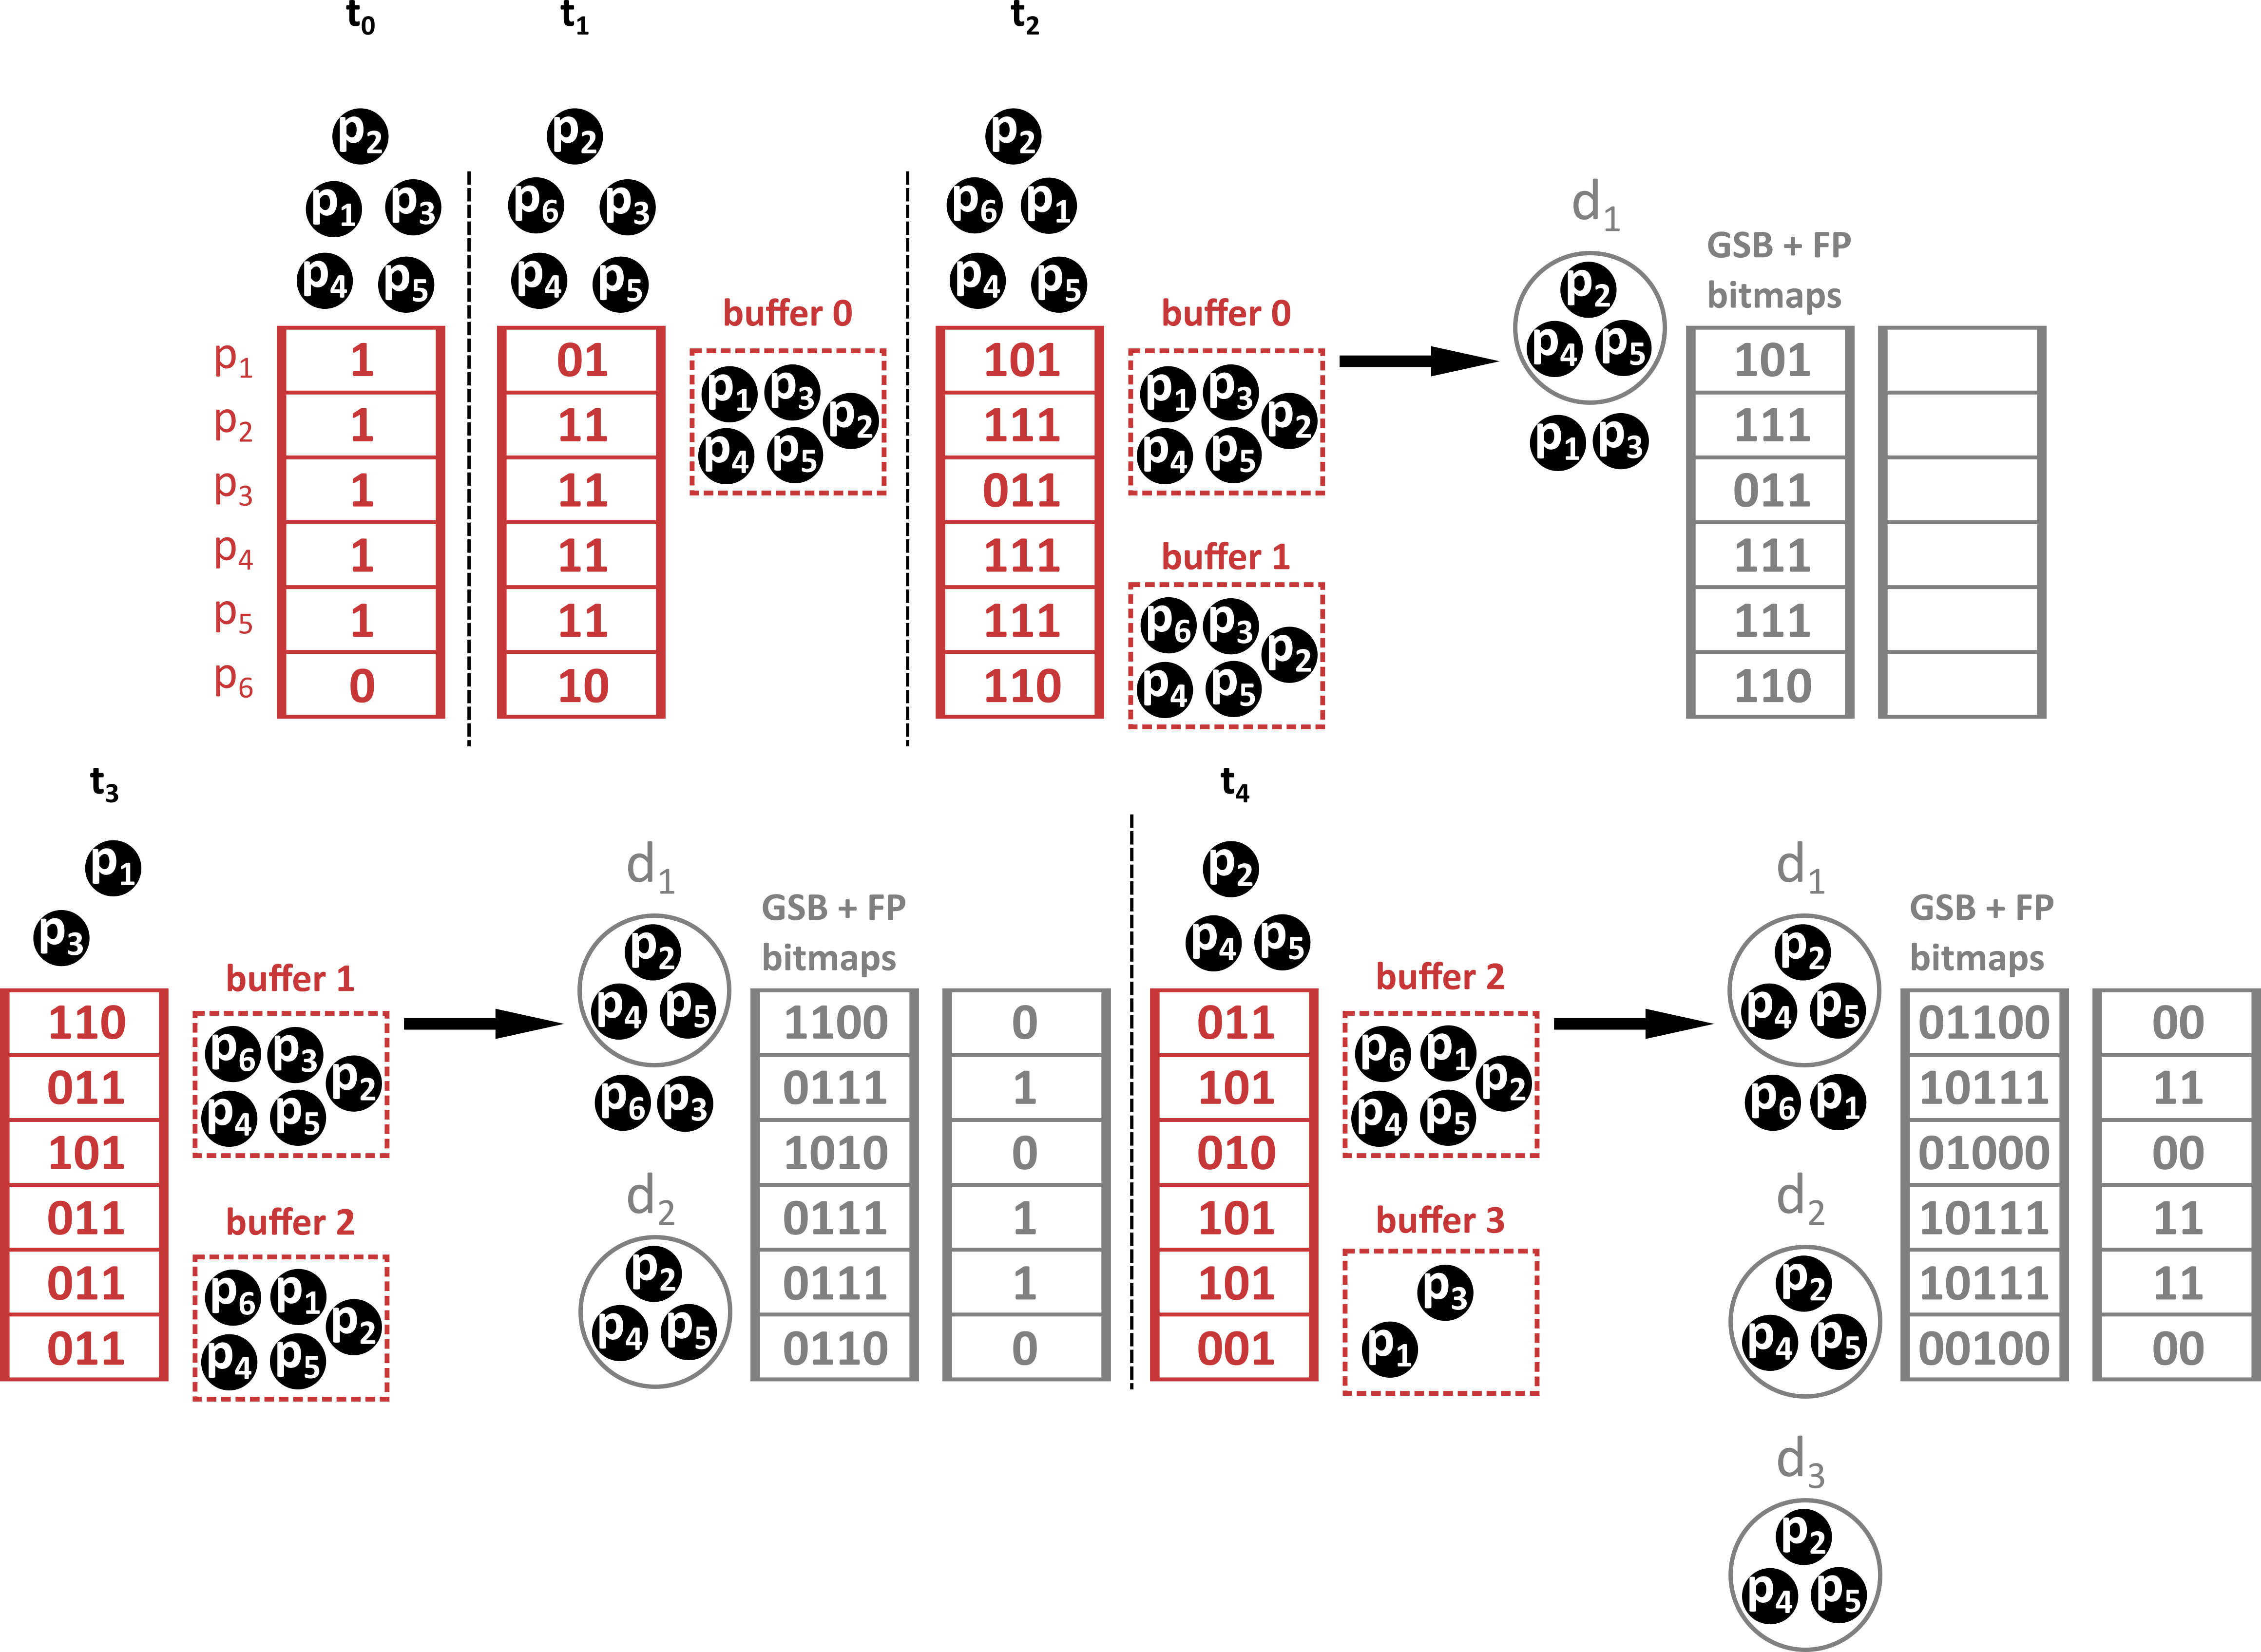
\includegraphics[width=\linewidth]{images/gsb_fp_flow.png}
    \label{fig:gsb_fp_flow}
\end{figure}

The same flow continues for time slot $t_3$, with GSB sending the buffered points from time slot $t_1$ to FP for
processing. We can now notice that the points that formed disk $d_1$ in the time slot $t_0$ now have a bit set to 1 in
their presence bitmaps in FP. It is worth noting how we perform the bitmap concatenation in FP (when it receives points
from $t_1$), in which the past time (FP bitmaps) goes at the right and the future (GSB bitmaps) goes at the left side of
the concatenated bitmap. We then perform a search for $\mu = 3$ bits set to 1 in that concatenated bitmaps to figure out
which points can potentially form a flock and can be places in a disk.

In time slot $t_4$, when FP receives the points from time slot $t_2$, a flock pattern will be found, since we could find
3 disks containing the same set of $O_{id}$ and containing at least $\mu = 3$ unique $O_{id}$.

\section{Taking advantage of Multi-core Architectures}
\label{sec:multithread}
Is well known that multi-core architectures are the current trend in technology. There is a myriad of multi-core
processors in the market and many chipset companies taking advantages of those processor architectures too (even small
devices, like smartphones, are being shipped with multi-core processors). Given that current scenario, there is no
excuse in not taking advantage of those mult-core processors and still executing our solution in a single process
fashion. Thus, we will remodel our propoesed architecture and in a multi-threaded structure and parallelize the tasks
that our algorithm is doing, in order to make it more responsive and fast so it can empower decision makers to act in
realtime.

One can see that the FP component, that we described in the previous section, is doing a lot of work in order to
discover the flock patterns, whenever it receives the set of points from the listener it perform the following actions:

\begin{enumerate}
    \item Build the whole point grid
    \item For each grid cell:
    \begin{enumerate}
        \item Get the Extended Grid Cell (EGC) (e.g. for cell $c_{x,y}$ it will get cells
            $c_{x - 1, y - 1}...c_{x + 1, y+ 1}$)
        \item Process the EGC, trying to cluster the points in disks
    \end{enumerate}
    \item Get the resulting disks and assure that there are no duplicates nor subsets of other disks
    \item Try to merge the disks with potential flocks from previous time slots
    \item Report new found flocks
\end{enumerate}

It can be easily perceived that the EGC processing (steps (a) and (b)) can be done in parallel for the multiple cells
that will be processed, since there is no dependency concurrent writing operations between cells. Another step that is
very CPU heavy is the one described in step 3, but that one is very difficult to parallelize, as we could see in
Algorithm~\ref{alg:fp}. In that algorithm we showed that we start with an empty set of disks in the beginning of the
\textsc{Process} procedure and add disks to that set as we go finding them. However, before adding a disk $d$ we check,
amongst the other disks that were previously there, if $d$ is neither a subset nor a superset of an existing disk. If
$d$ is a subset, than it is not added, but if $d$ is superset of an existing disk $d_2$, that disk $d_2$ is then removed
from the set and $d$ is added instead (the superset check is done inside the procedure \textsc{AddDisk}). Thus, if we
try to parallelize that disk check procedure we would need to have synchronizing primitives to protect the concurrent
writing operations to the shared disk set, which could end up being more slow than executing it sequentially. Even
without being able to fully parallelize the disk check steps we can still take advantage of other techniques to gain
some speed in processing, like using the divide and conquer approach. The idea would be to have multiple disks sets (one
per independent worker thread processing EGCs) and have each independent thread add disks (and thus check for
subsets/supersets) to its own set. When each worker thread has finished its processing we would have each thread's set
being merged with the global disk set in FP. leaving less checks to be performed by the global disk set.

\subsection{Multi-threaded Design}
\label{subsec:multithread}
The multi-threaded idea described in \secref{sec:multithread} can be modeled as a Producer-Multiple Consumers problem,
where we would have a single producer assembling the EGCs and multiple consumers taking a EGC from a shared queue and
clustering the points in the disks that it might find in that specific EGC. On a step further, each consumer thread
$c_t$ will also spawn another thread $d_t$ that will process disks that $c_t$ has found and will check for subsets and
supersets in its own private disk set.

\begin{figure}[h!]
    \centering
    \caption{Modeling the FP in a Producer-Multiple Consumers architecture}
    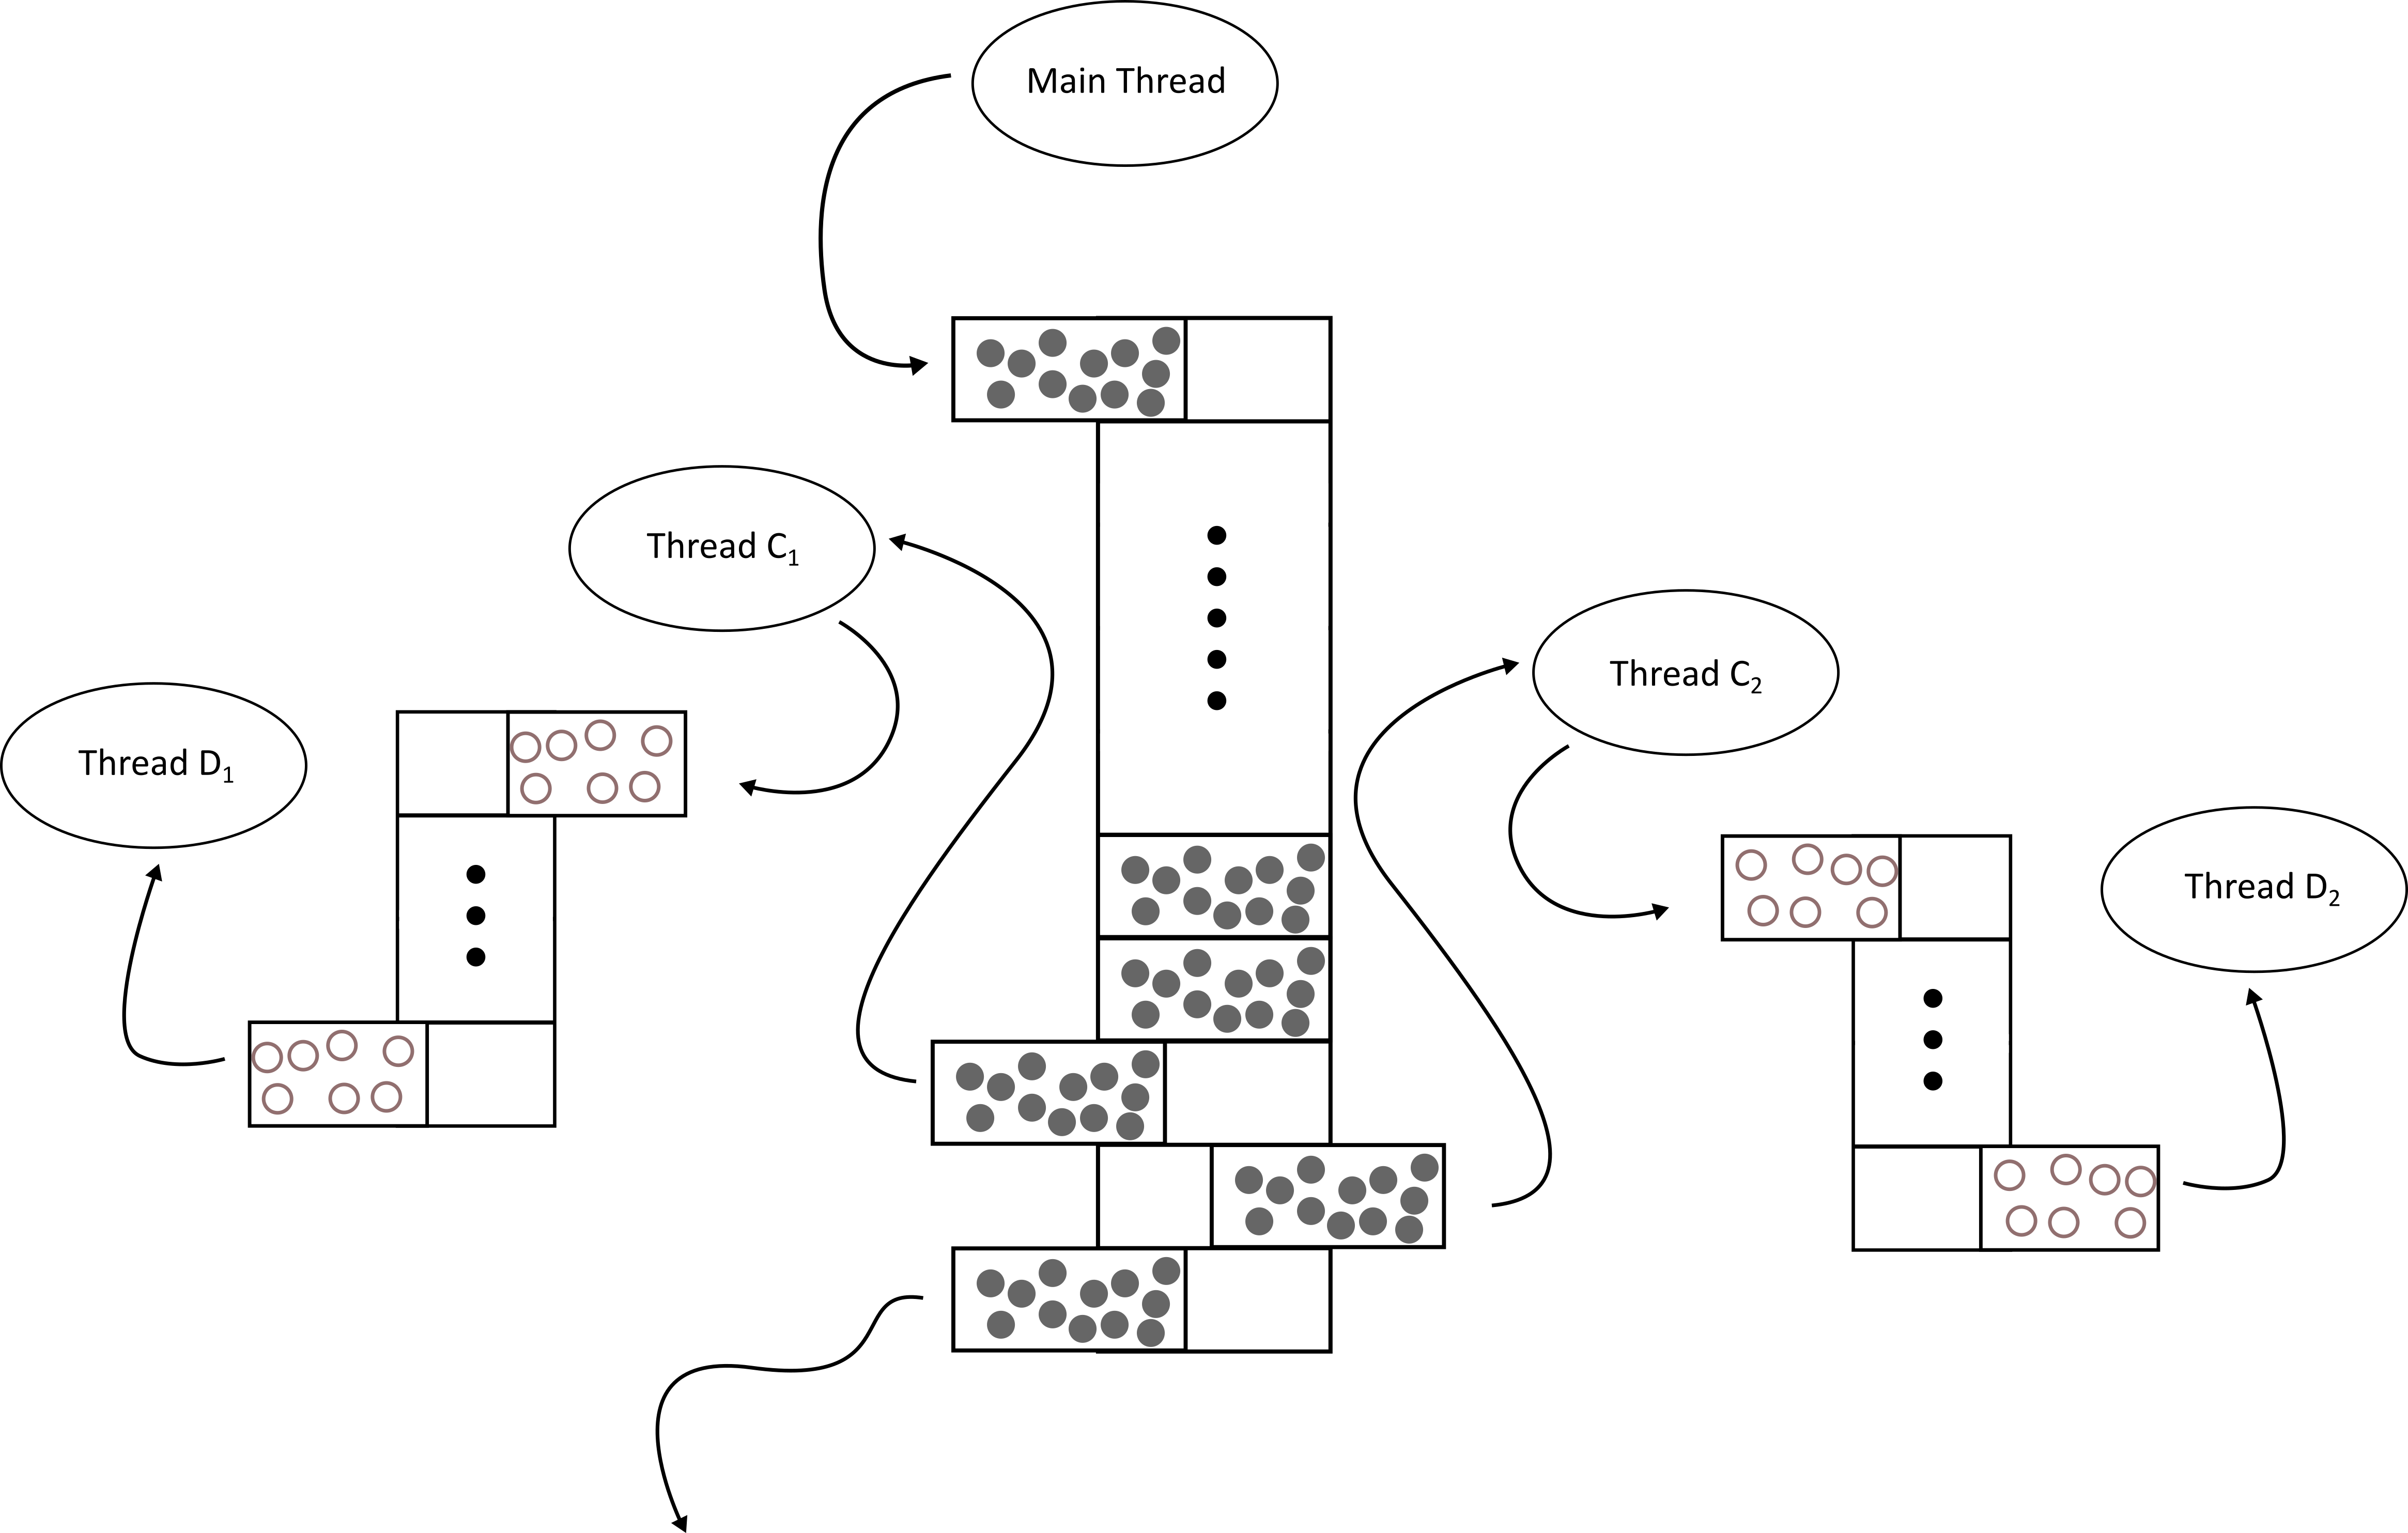
\includegraphics[width=\linewidth]{images/multithread.png}
    \label{fig:multithread}
\end{figure}

\figref{fig:multithread} illustrates how the FP will be rearchitected in order to take advantage of parallel execution.
We can see that the main thread will collect the EGC for each cell grid and enqueue it in a shared queue that will be
acessed by $N$ consumers. Whenever a consumer ($c_t$ thread) dequeues an EGC, it will then try to find a pair of disks
for each pair of points in the EGC, cluster the remaining points in those disks and then enqueue those disks in another
shared queue. Such shared queue will only be shared with the disk thread $d_t$ belonging to the $c_t$ thread that
created it. Then, each $d_t$ will be responsible to check for subsets and supersets in its own set of disks, saving a
lot of processing time when those disks will be merged (and also checked for subsets and supersets) with the global disk
set in the \textsc{Process} procedure.

\chapter{Experimental Results}
\label{chp:results}
As explained in \chapref{chp:techbackground}, the flock pattern detection relies mainly in 3 parameters, namely
\textit{number of trajectories} ({$\mu$), \textit{flock extension (or length)} ($\delta$) and \textit{disk radius}
($\epsilon/2$). Those parameters impact significantly in the number of patterns found as well as the time taken to find
those patterns, depending on the dataset being analyzed. To validate the efficiency of \ac{bitdf}, we chose 4 datasets
referred by Zheng \citep{survey}, that are being widely used in trajectory data mining researches in the academia. Of
those 4 datasets, 2 were collected from real-world experiments and 2 were synthetic generated.

Before evaluating the performance of \ac{bitdf} using those datasets, we first gathered some metadata information about
them, in order to choose wisely the value for the aforementioned parameters, so we could indeed find a good number of
flocks patterns. Such metadata were collected by running \ac{bitdf} multiple times with various values for those
parameters. Thus, based on the dataset description, we picked some starting values for them and then increased or
decreased the values according to the number of flock patterns that we were able to find. After finding at least 100
flock patterns, we then settled on a range of values for those parameters and used them to evaluate each dataset.

\figref{fig:experimental_arch} shows the components (using the architecture proposed in \secref{sec:architecture}) that
will be part of our experiments and how our experiments are going to be performed. For each dataset (which will be
presented individually in the sections to come) that we used, we simulated an online stream of \ac{gps} data arriving on
a custom \ac{dsc} in our system. Then, that incoming \ac{gps} data would be forwarded to a \ac{dd} that knows how to
translate each entry in that specific dataset to a structure that can be understood by the \ac{gsb} \ac{dl}. When the
\ac{gsb} \ac{dl} gets the data, the \algoref{alg:gpsb} will take care of it, buffering it and building the necessary
presence bitmap for that $O_{id}$. After we have buffered $\delta$ time slots of points in \ac{gsb}, the next
destination of the \ac{gps} data is the \ac{fp} \ac{dp}, which is composed by three different components:

\begin{enumerate}
    \item \textbf{Grid Manager}: Will get the \ac{gps} data and build the grid depicted in \figref{fig:grid} and provide
        the \ac{egc} for each grid cell.
    \item \textbf{Disk Manager}: Gets each disk generated by \ac{fp} and will check for duplicates/superset disks and
        add it to the global disk set if that disk is unique.
    \item \textbf{Flock Manager}: Stores the potential flock patterns from previous time slots and merges the disks
        generated by the current time slot in order to find new flock patterns.
\end{enumerate}

\begin{figure}[h!]
    \centering
    \caption{System design implemented for the experiments}
    \centerline{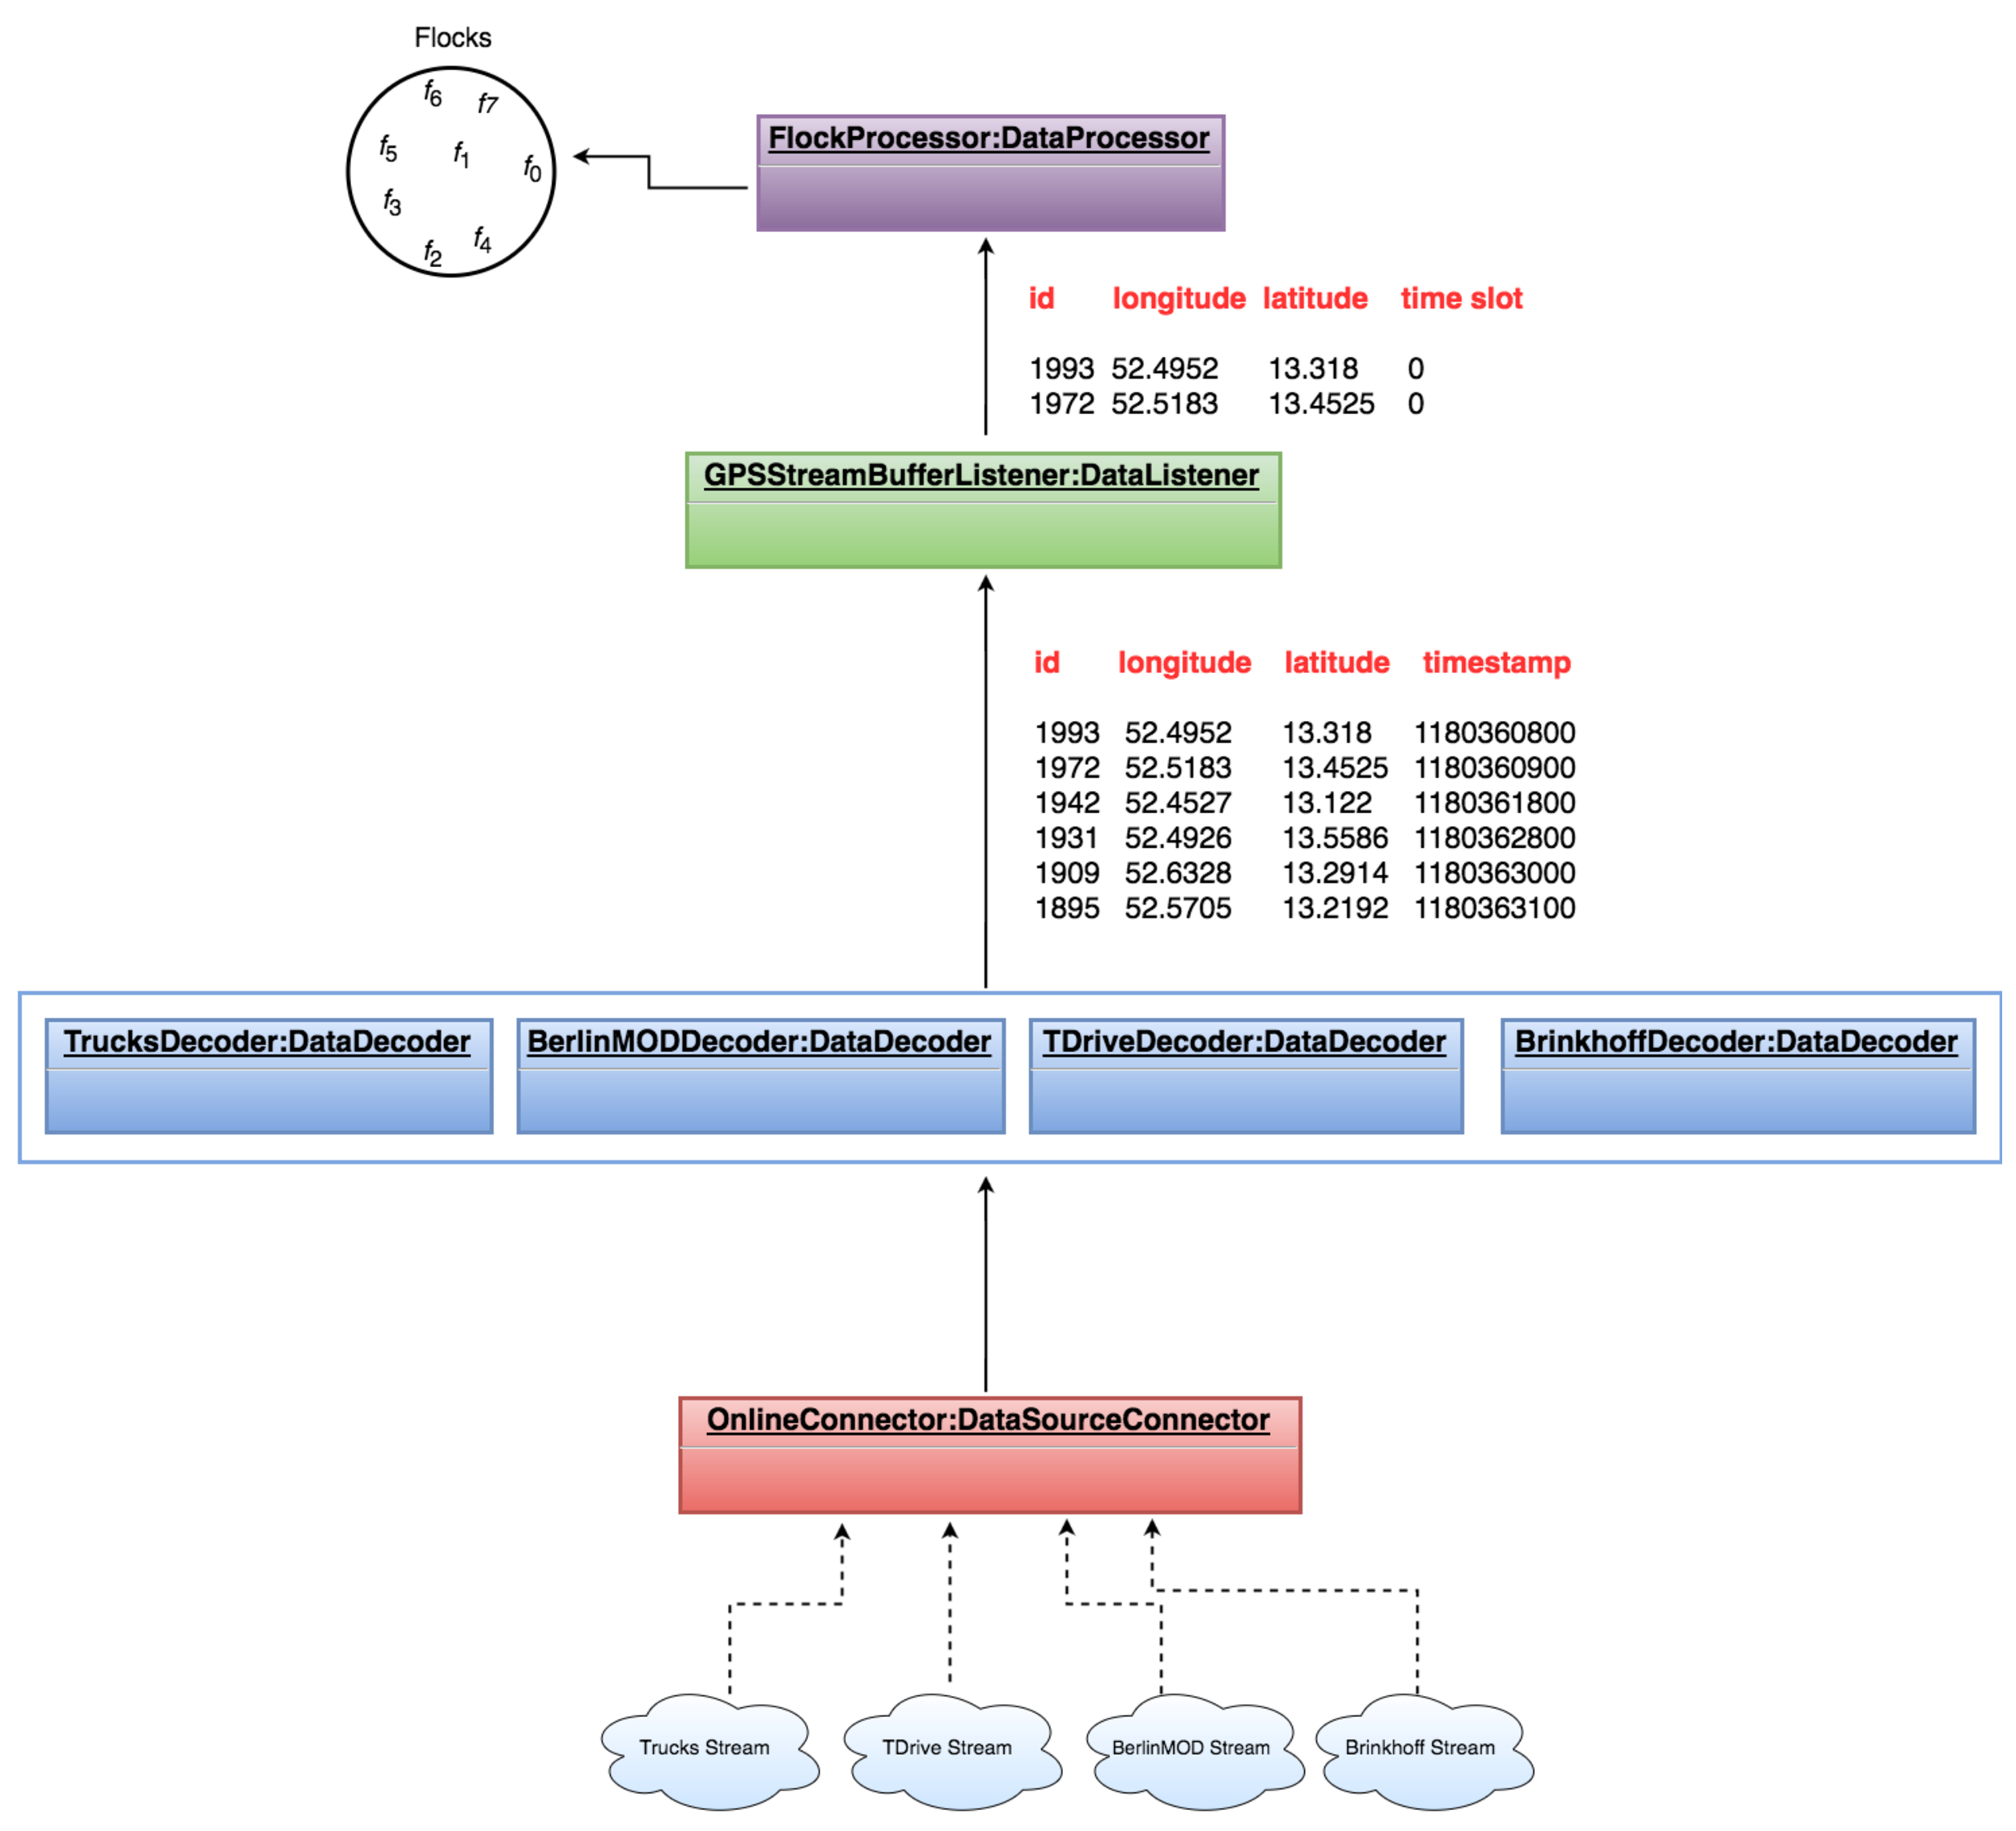
\includegraphics[width=\textwidth]{images/experimental_arch.eps}}
    \footnotesize{Source: Made by the author.}
    \label{fig:experimental_arch}
\end{figure}

The metrics that we chose to measure the efficiency of \ac{bitdf} were (1) Running Time and (2) Number of Disks
Generated. For (1) we went through each parameter ($\mu$, $\delta$ and $\epsilon$), fixed it in a specific value and
varied the remaining others based on the range that we settled from our metadata gathering. We picked (2) as an
evaluation metric because it will show with numbers the reason why \ac{bitdf} can run way faster than the other
algorihtms. Finally, in order to have a baseline to compare against \ac{bitdf}, we implemented the \ac{bfe} algorihtm
proposed by Vieira et al. \citep{vieira} and ran benchmarks with it as well.

We implemented the system architecture proposed in \figref{fig:experimental_arch} in C++, using g++ 4.8.4 and the C++11
\citep{cpp11spec} features. Our test machine used to run our performance experiments was a Linux box with Intel Xeon
Quad processor and 14GB of main memory running Ubuntu Server 14.04 \ac{lts}. As already mentioned, we used four datasets
(real and synthetic) in our experiments, with some of them having more than 50M entries and 2K unique $O_{id}$.

Before showing the results, there are some \ac{ao} that will hold for any dataset being analyzed here:

\begin{enumerate}
    \item \textbf{$\delta$ variation}: The longer the flock patterns we try to find (long $\delta$), the more disks will
        stay cached being analyzed and trying to be merged with new disks from time slots to come. This can have a big
        impact in running time.\label{sssec:lvariation}

    \item \textbf{$\epsilon$ variation}: As the disk radius ($\epsilon / 2$) gets bigger, more points will be clustered
        inside a disk and thus more intersections and duplicates of those disks as more likely to be found. This will
        affect the time spent in analyzing disks from one time slot to another. \label{sssec:gvariation}

    \item \textbf{$\mu$ variation}: By increasing $\mu$, it gets more and more difficult to find disks that are flock
        candidates ($|d| \ge \mu$), so less disks are generated. This scenario is where \ac{bitdf} will achieve less
        improvements. \label{sssec:nvariation}
\end{enumerate}

\section{Trucks Dataset}
\label{sec:trucks}
This was one of the datasets that Vieira et al. \citep{vieira} used in the experiments of \ac{bfe}, but the authors
modified such dataset \citep{trucksdataset}, resulting in a dataset which is way far from those found in real-world
analyses. In their modification, every time interval is of one second, the \ac{gps} coordinates were mapped to a
$\mathbb{R}^2$ coordinate system (ranging from 0 to 1000) and most of the points are present in each time interval. The
modified dataset resulted in 112203 entries and 276 unique $O_{id}$ (instead of 50 in the original dataset).

\begin{figure*}[h!]
    \centering
    \caption{Results varying $\delta$ and $\epsilon$ for Trucks dataset}
    \begin{subfigure}[t]{0.48\textwidth}
        \caption{$\mu = 4$, $\epsilon = 1.5$ and $\delta$ varying}
        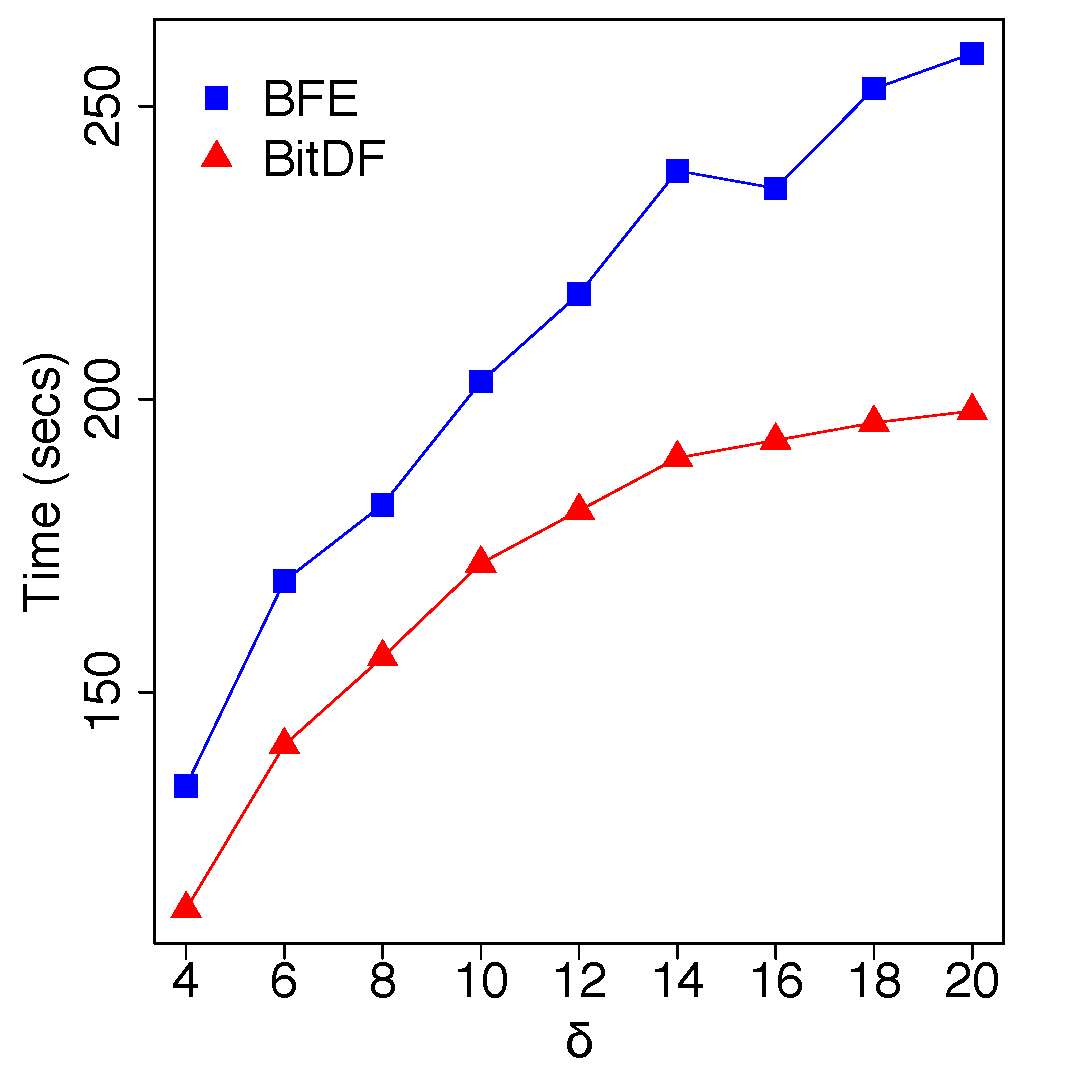
\includegraphics[width=\textwidth]{images/Trucks_n_4_g_1_5_varying_l.eps}
        \label{fig:trucks_vary_l}
    \end{subfigure}
    \begin{subfigure}[t]{0.48\textwidth}
        \caption{$\mu = 4$, $\delta = 20$ and $\epsilon$ varying}
        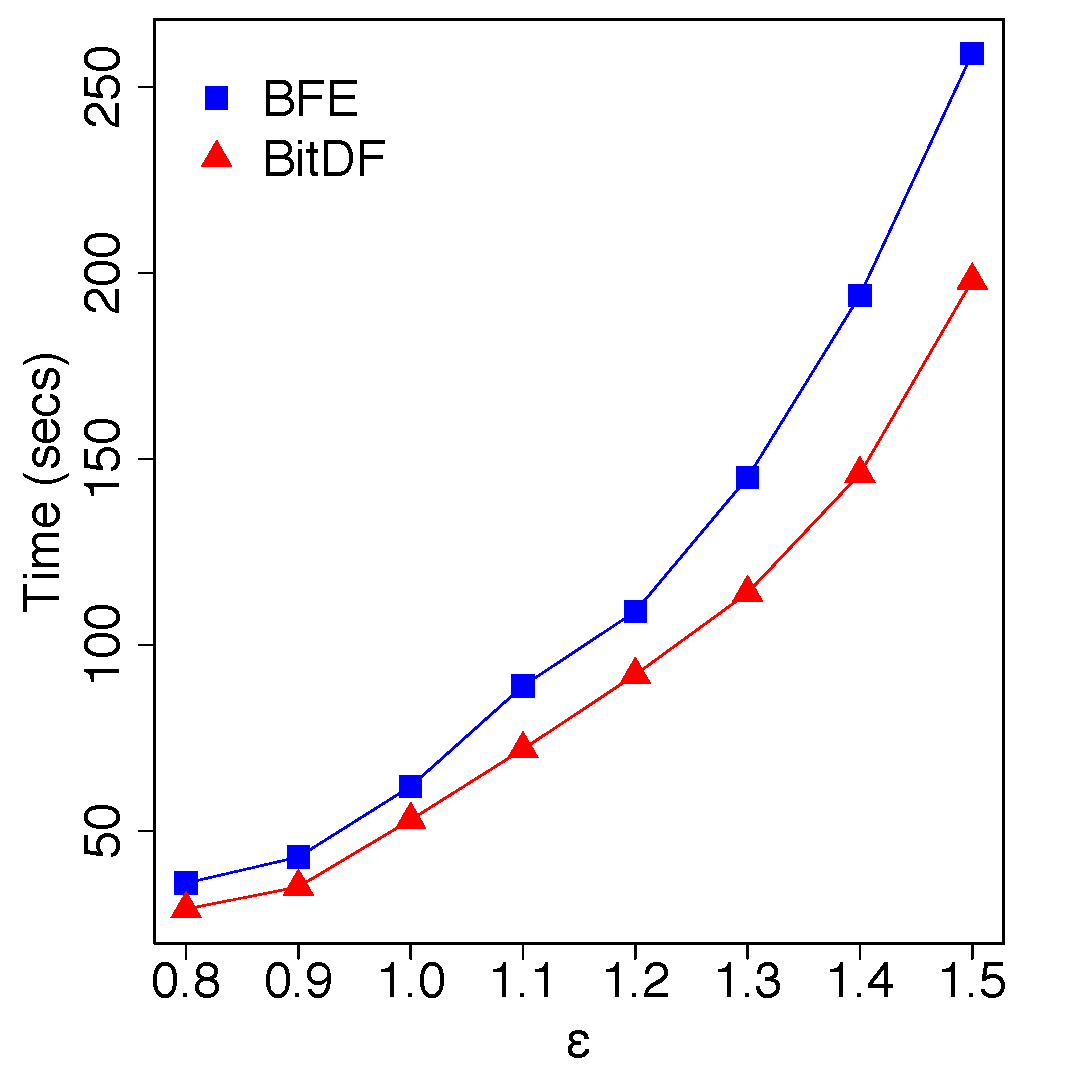
\includegraphics[width=\textwidth]{images/Trucks_n_4_l_20_varying_g.eps}
        \label{fig:trucks_vary_g}
    \end{subfigure}
    \label{fig:trucks_results}
    \footnotesize{Source: Made by the author.}
\end{figure*}

\begin{figure*}[h!]
    \centering
    \caption{Results varying $\mu$ and number of disks generated over time for Trucks dataset}
    \begin{subfigure}[t]{0.48\textwidth}
        \caption{$\delta = 20$, $\epsilon = 1.5$ and $\mu$ varying}
        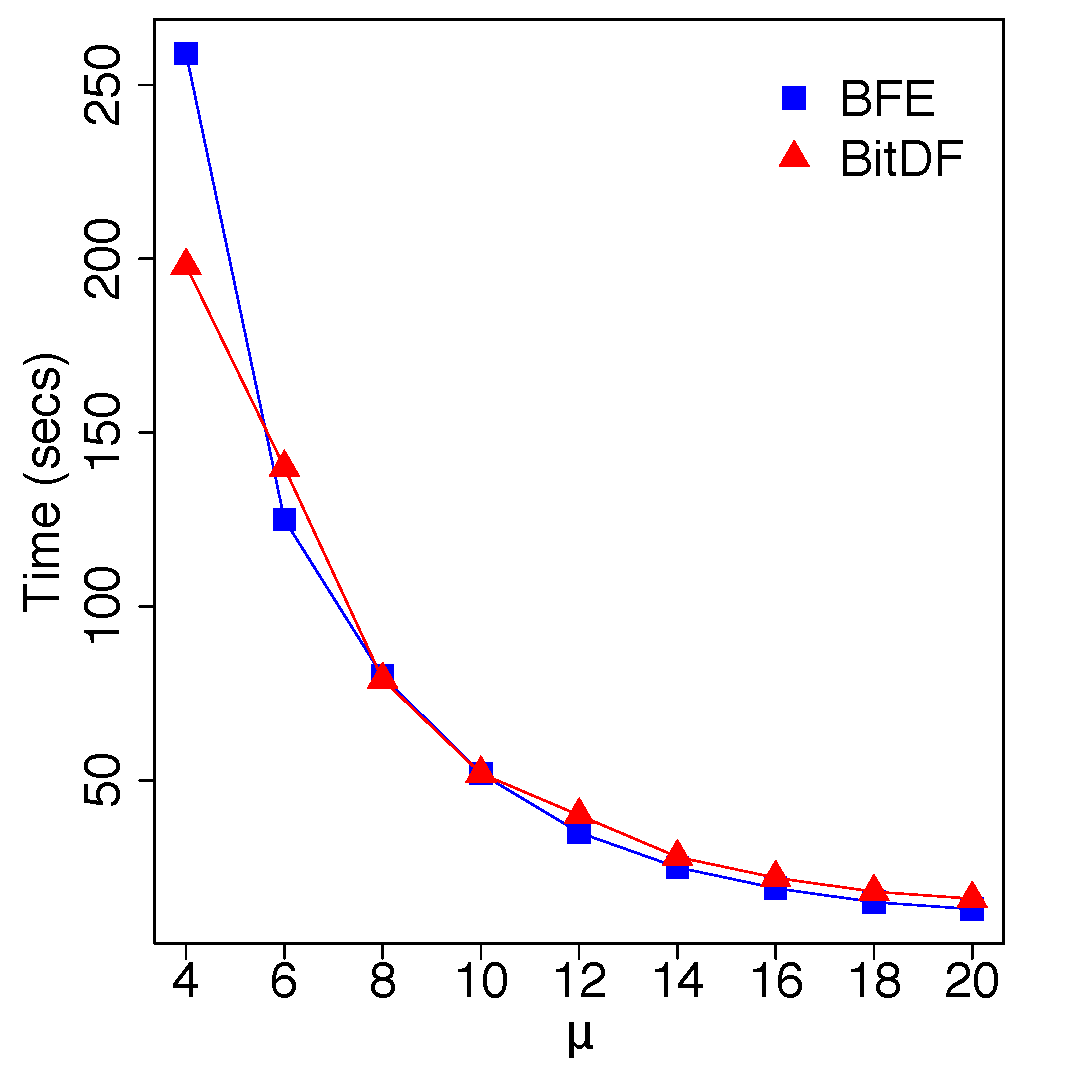
\includegraphics[width=\textwidth]{images/Trucks_l_20_g_1_5_varying_n.eps}
        \label{fig:trucks_vary_n}
    \end{subfigure}
    \begin{subfigure}[t]{0.48\textwidth}
        \caption{Cumulative disks by time}
        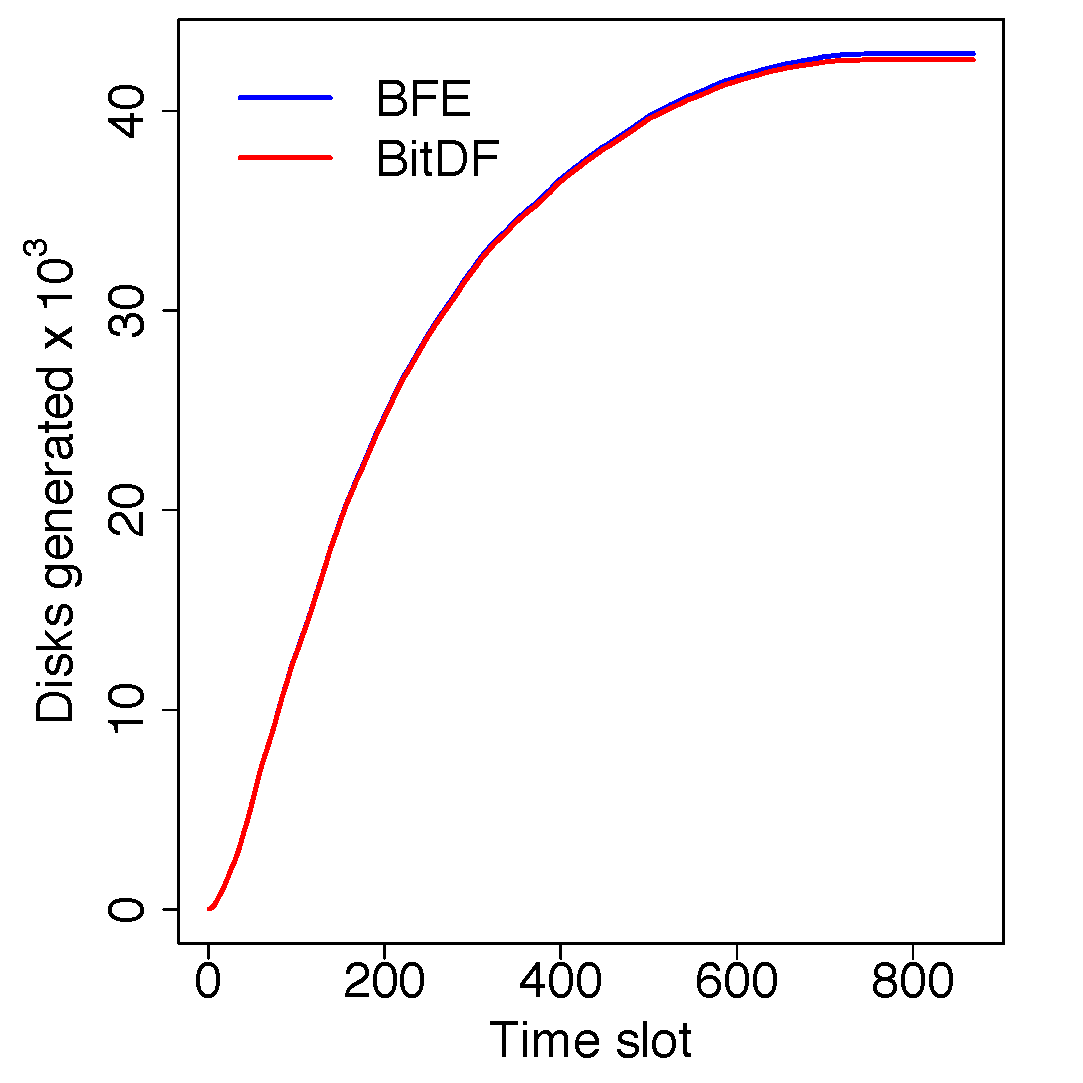
\includegraphics[width=\textwidth]{images/Trucks_d.eps}
        \label{fig:trucks_disks}
    \end{subfigure}
    \footnotesize{Source: Made by the author.}
    \label{fig:trucks_results2}
\end{figure*}

By looking at \figref{fig:trucks_results} and \figref{fig:trucks_results2}, we can see that \ac{bitdf} had some gains in
execution time. However, they were not too significant due to the fact that the number of disks generated by each time
slot does not differ too much between \ac{bfe} and \ac{bitdf}, as we can see in \figref{fig:trucks_disks}. This happens
because almost all points appear in every single time slot, then buffering and mapping the $O_{id}$ presence in time
does not make a big impact, since we will not be able to filter out disks created with points not being present in
$\delta$ consecutive time slots. \figref{fig:trucks_vary_l} and \figref{fig:trucks_vary_g} show some running time
improvements against \ac{bfe}, which are backed up by the explanations given at \ac{ao}~\ref{sssec:lvariation} and
\ac{ao}~\ref{sssec:gvariation}. A different behavior is observed in \figref{fig:trucks_vary_n}, in which \ac{bitdf}
starts better but ends up almost tied with \ac{bfe}, which can be explained by \ac{ao}~\ref{sssec:nvariation}, but is
also very influenced by the dataset modifications.
\vfill

\section{BerlinMOD Dataset}
\label{sec:berlinmod}
BerlinMOD consists in a traffic generation model \citep{berlinmodpaper} used to create sythentic datasets of \acp{mo}.
This particular dataset that we are analysing was the biggest one that we could find in the set of synthetic datasets
that are available in their website \citep{berlinmod} and consists of 56,127,943 entries and 2000 unique $O_{id}$.

\begin{figure*}[h!]
    \centering
    \caption{Results varying $\delta$ and $\epsilon$ for BerlinMOD dataset}
    \begin{subfigure}[t]{0.48\textwidth}
        \caption{$\mu = 4$, $\epsilon = 100$ and $\delta$ varying}
        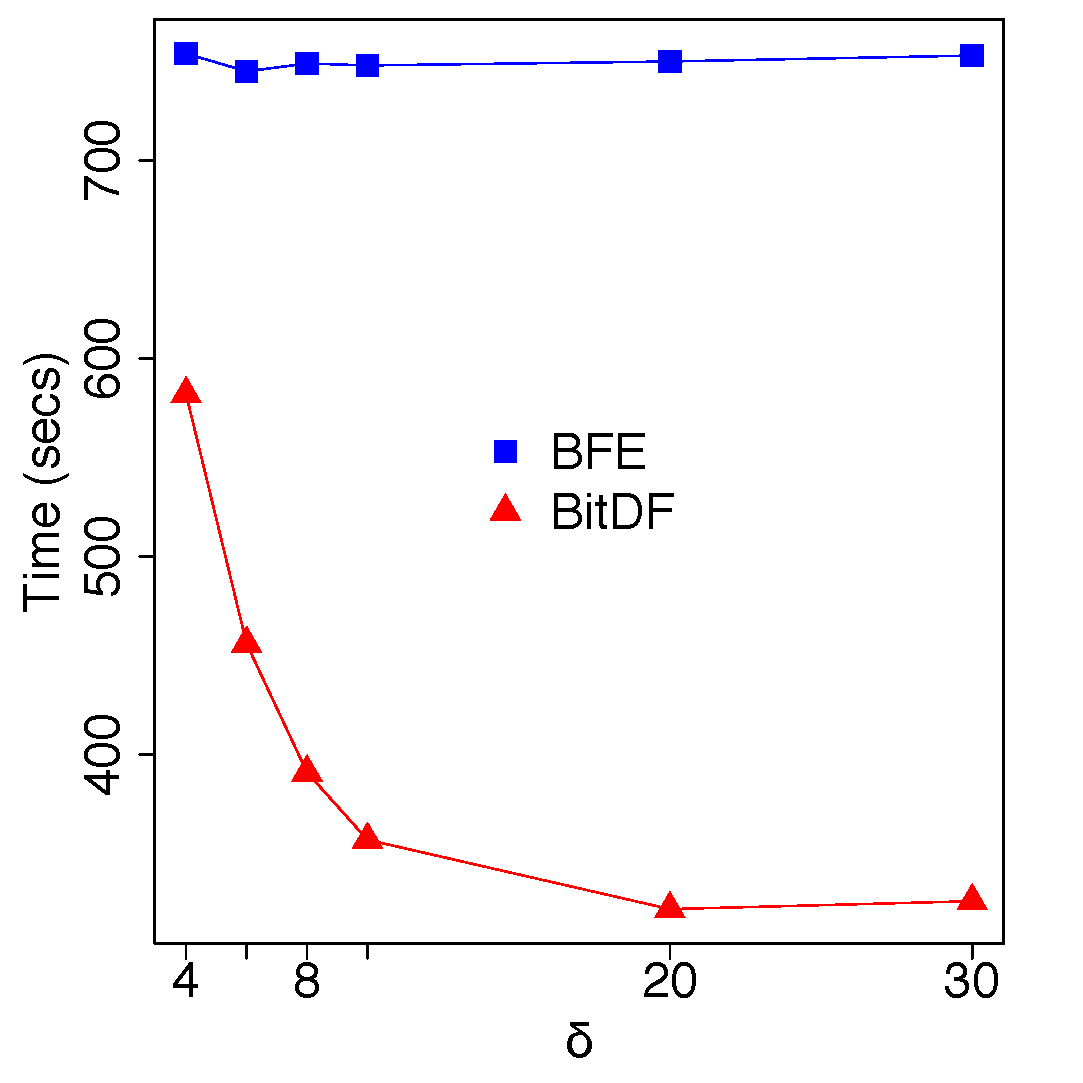
\includegraphics[width=\textwidth]{images/BerlinMOD_n_4_g_100_varying_l.eps}
        \label{fig:berlinmod_vary_l}
    \end{subfigure}
    \begin{subfigure}[t]{0.48\textwidth}
        \caption{$\mu = 4$, $\delta = 8$ and $\epsilon$ varying}
        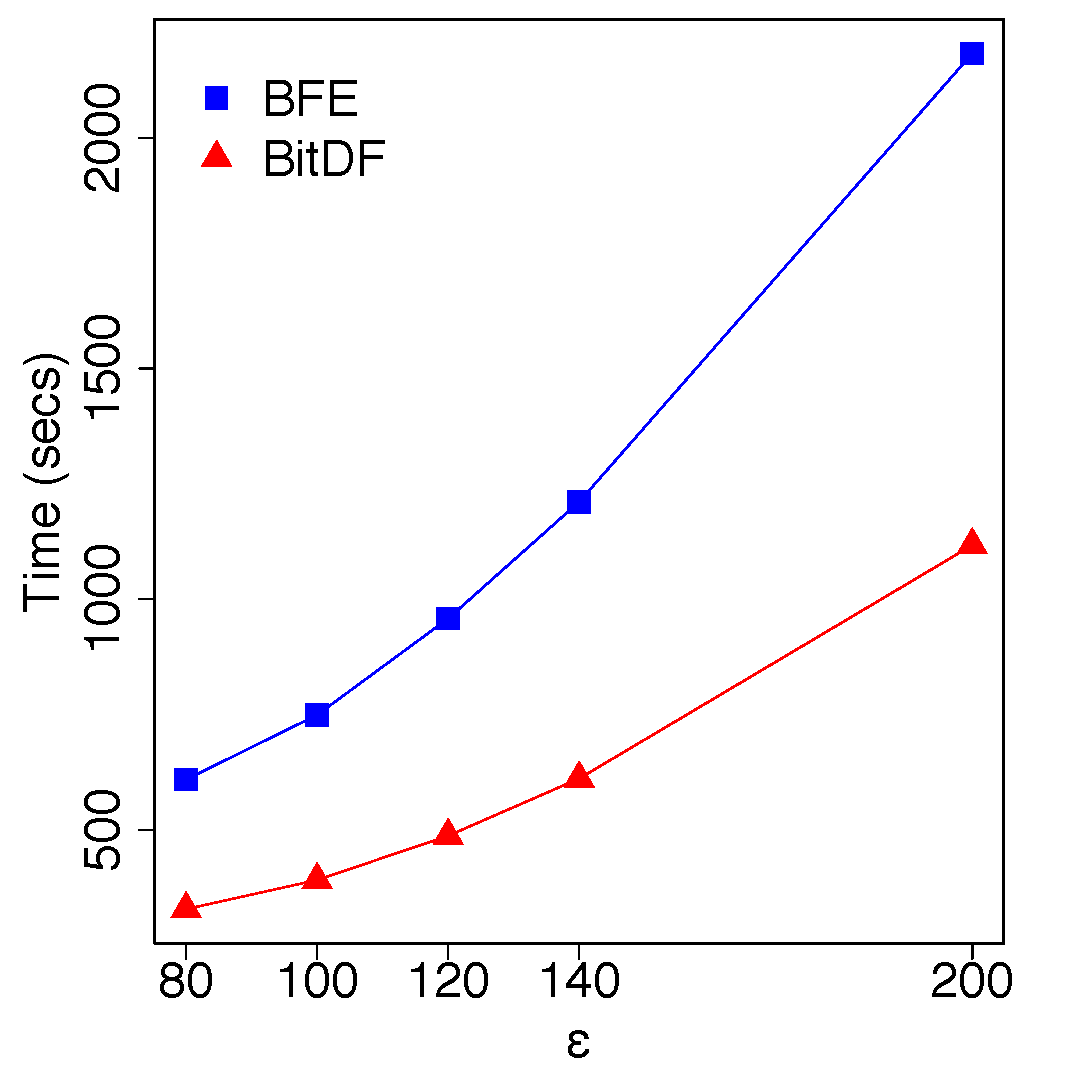
\includegraphics[width=\textwidth]{images/BerlinMOD_n_4_l_8_varying_g.eps}
        \label{fig:berlinmod_vary_g}
    \end{subfigure}
    \footnotesize{Source: Made by the author.}
    \label{fig:berlinmod_results}
\end{figure*}

\begin{figure*}[h!]
    \centering
    \caption{Results varying $\mu$ and number of disks generated over time for BerlinMOD dataset}
    \begin{subfigure}[t]{0.48\textwidth}
        \caption{$\delta = 8$, $\epsilon = 100$ and $\mu$ varying}
        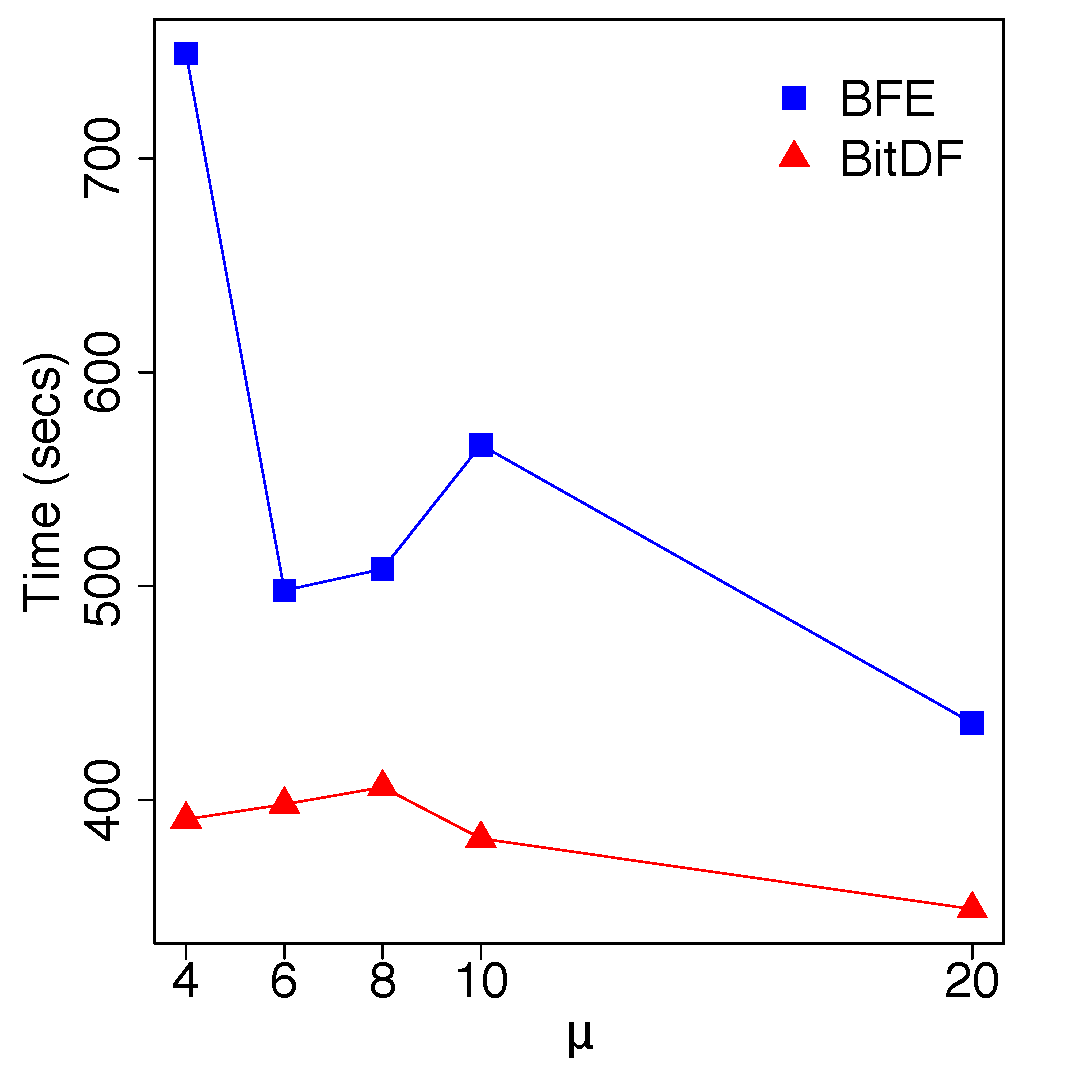
\includegraphics[width=\textwidth]{images/BerlinMOD_l_8_g_100_varying_n.eps}
        \label{fig:berlinmod_vary_n}
    \end{subfigure}
    \begin{subfigure}[t]{0.48\textwidth}
        \caption{Cumulative disks by time}
        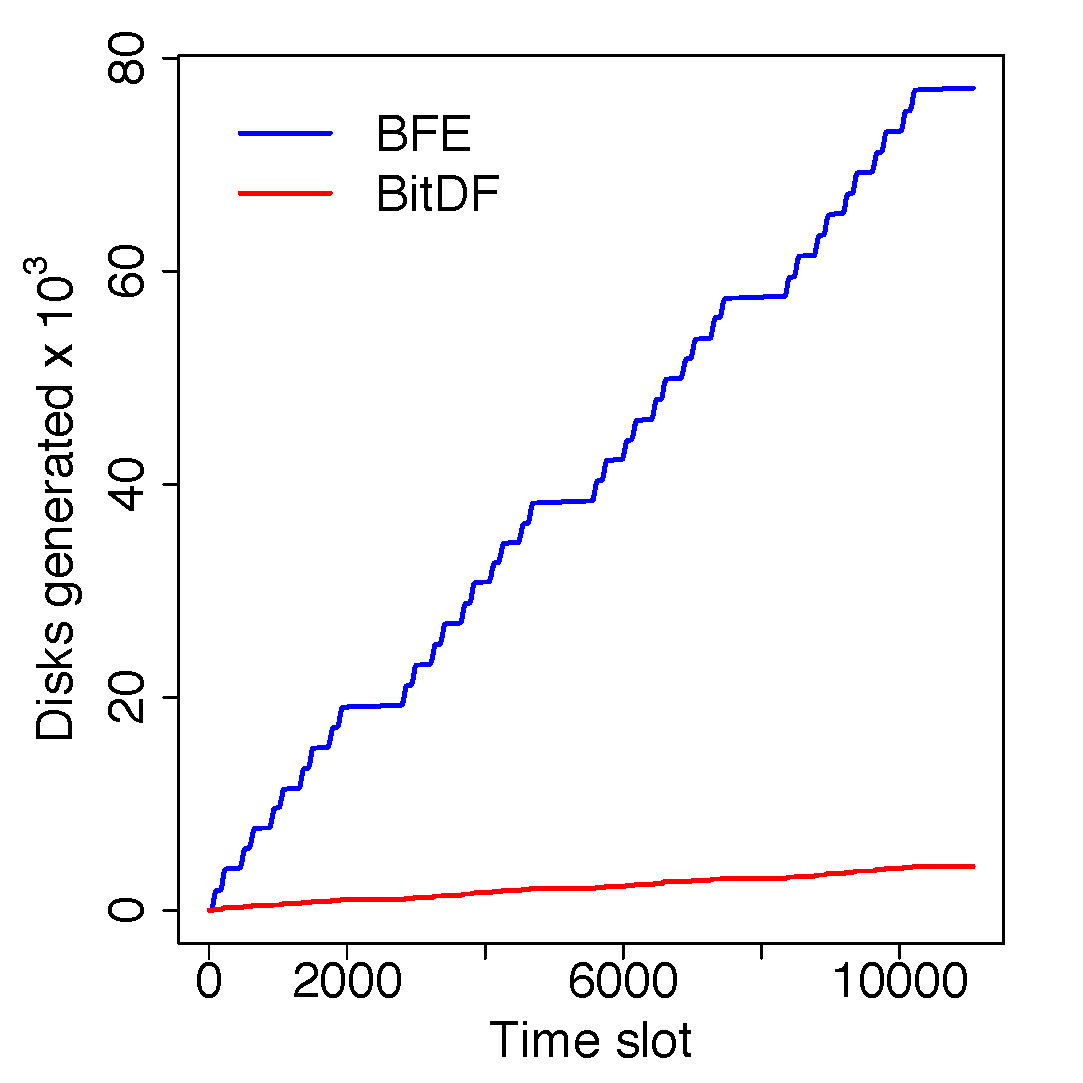
\includegraphics[width=\textwidth]{images/BerlinMOD_d.eps}
        \label{fig:berlinmod_disks}
    \end{subfigure}
    \footnotesize{Source: Made by the author.}
    \label{fig:berlinmod_results2}
\end{figure*}

As we can see by the results presented in \figref{fig:berlinmod_results} and \figref{fig:berlinmod_results2}, \ac{bitdf}
was able to achieve great performance gains over \ac{bfe}, in some cases being 57\% faster
(\figref{fig:berlinmod_vary_l}). In \figref{fig:berlinmod_disks} it is shown that \ac{bitdf} reduces the cumulative
number of disks created over time in 94\%, by only creating disks that can indeed form flock patterns, which justifies
the great improvements that \ac{bitdf} was able to get in this dataset. Differently from the results presented in
\secref{sec:trucks}, \ac{bitdf} was able to get great improvements over \ac{bfe}, ranging from 20\% to 48\%, even when
increasing the value of $\mu$ as depicted in \figref{fig:berlinmod_vary_n}. Lastly, as depicted in
\figref{fig:berlinmod_vary_g}, \ac{bitdf} was able to outperform \ac{bfe} in almost 50\% when varying the parameter
$\epsilon$.

\section{TDrive Dataset}
\label{sec:tdrive}
This is a real dataset, having spatio-temporal data describing one week of trajectories of taxis in Beijing, China,
available in \citep{tdrive}. It has 17,762,489 entries with 10336 unique $O_{id}$.

\begin{figure*}[h!]
    \centering
    \caption{Results varying $\delta$ and $\epsilon$ for TDrive dataset}
    \begin{subfigure}[t]{0.48\textwidth}
        \caption{$\mu = 4$, $\epsilon = 100$ and $\delta$ varying}
        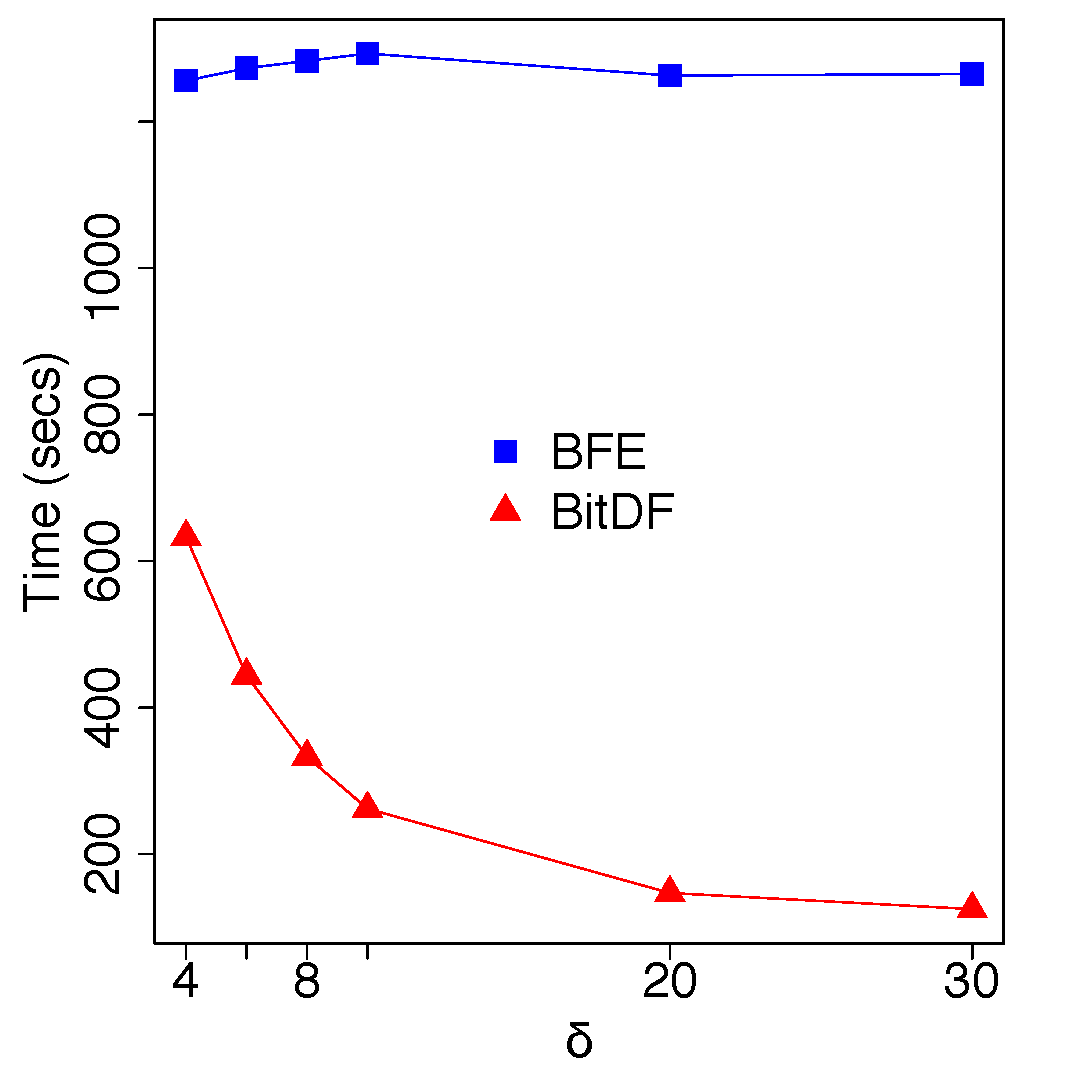
\includegraphics[width=\textwidth]{images/TDrive_n_4_g_100_varying_l.eps}
        \label{fig:tdrive_vary_l}
    \end{subfigure}
    \begin{subfigure}[t]{0.48\textwidth}
        \caption{$\mu = 4$, $\delta = 8$ and $\epsilon$ varying}
        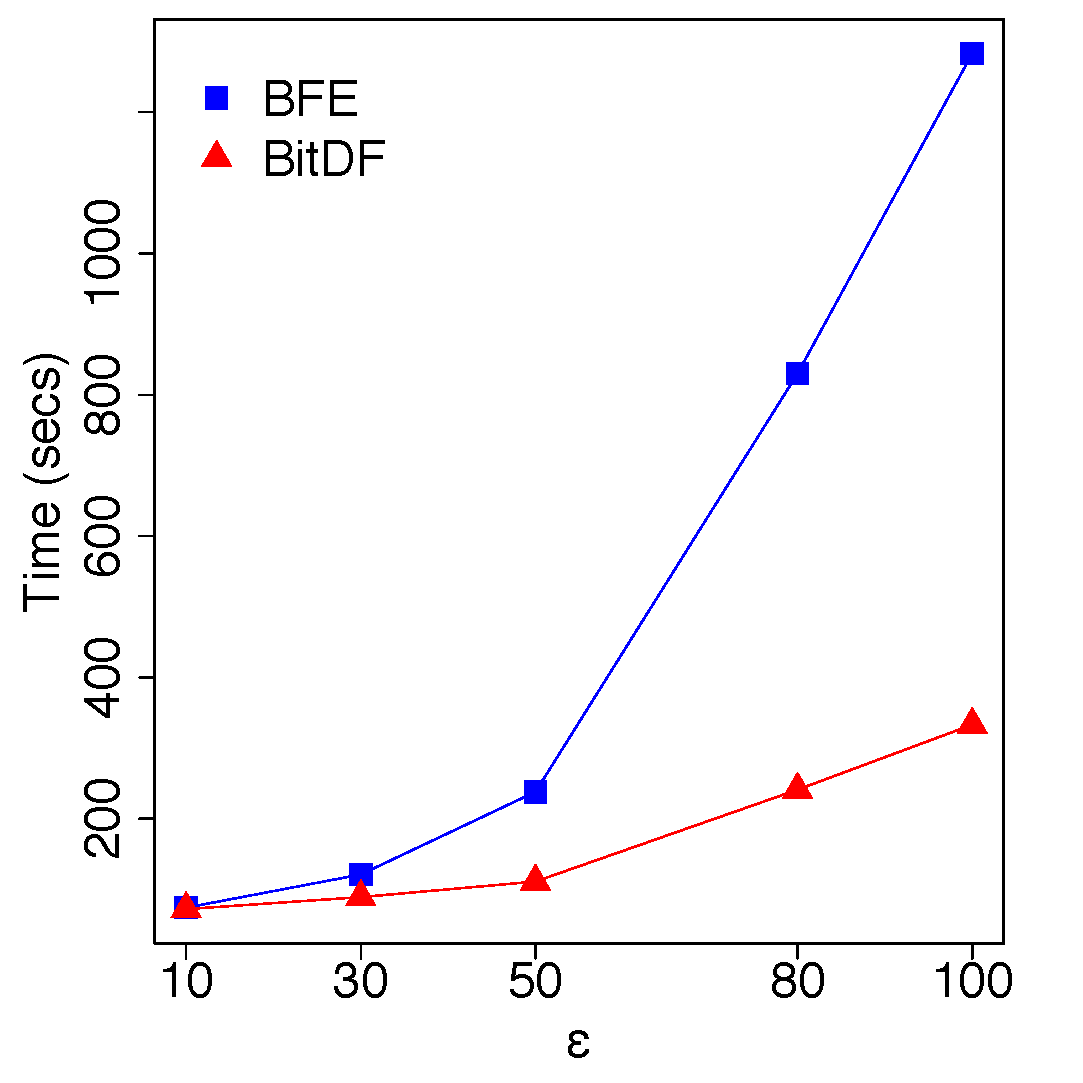
\includegraphics[width=\textwidth]{images/TDrive_n_4_l_8_varying_g.eps}
        \label{fig:tdrive_vary_g}
    \end{subfigure}
    \footnotesize{Source: Made by the author.}
    \label{fig:tdrive_results}
\end{figure*}

One can see by the results presented in \figref{fig:tdrive_results} and \figref{fig:tdrive_results2}, that \ac{bitdf}
was able to dramatically reduce the execution time, when compared to \ac{bfe}. When varying the $\delta$ parameter, the
running time improvement was of almost 90\%, droping from 1,265 seconds to only 125 seconds of processing time, as shown
in \figref{fig:tdrive_vary_l}. Continuing the improvements, in \figref{fig:tdrive_vary_g} we can see that \ac{bitdf}
reduced the execution time up to 74\% when varying $\epsilon$. Additionally, despite seeing some similar behavior with
the other analyzed datasets (like presented in \secref{sec:trucks}) when varying $\mu$, \figref{fig:tdrive_vary_n} shows
that \ac{bitdf} was able to improve the execution time by 74\% in some cases. It is also worth noting that the results
achieved are a reflex of the huge decrease of disks that were generated by time, as depicted in
\figref{fig:tdrive_disks}, reaching almost 96\% of reduction.

\begin{figure*}[h!]
    \centering
    \caption{Results varying $\mu$ and number of disks generated over time for TDrive dataset}
    \begin{subfigure}[t]{0.48\textwidth}
        \caption{$\delta = 8$, $\epsilon = 100$ and $\mu$ varying}
        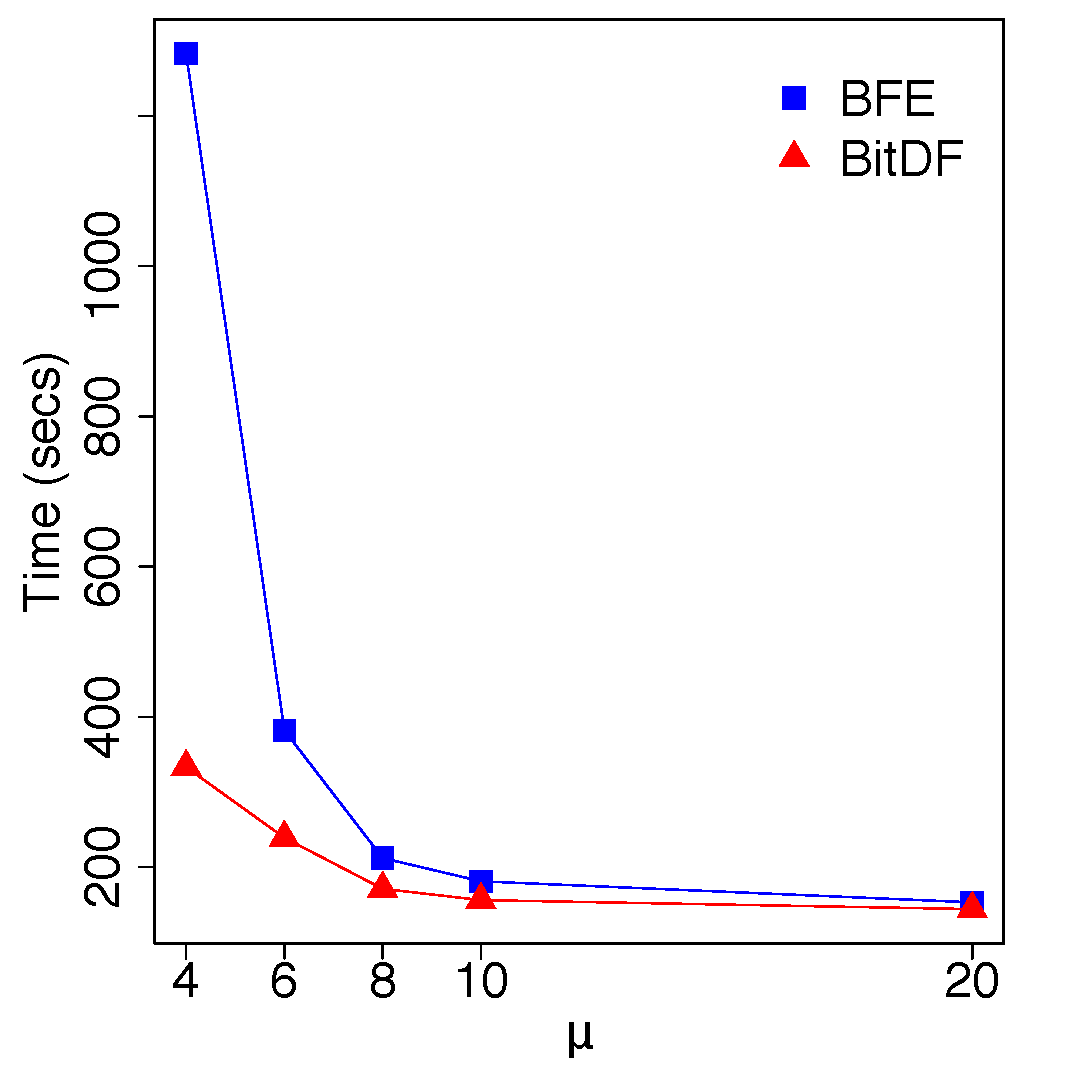
\includegraphics[width=\textwidth]{images/TDrive_l_8_g_100_varying_n.eps}
        \label{fig:tdrive_vary_n}
    \end{subfigure}
    \begin{subfigure}[t]{0.48\textwidth}
        \caption{Cumulative disks by time}
        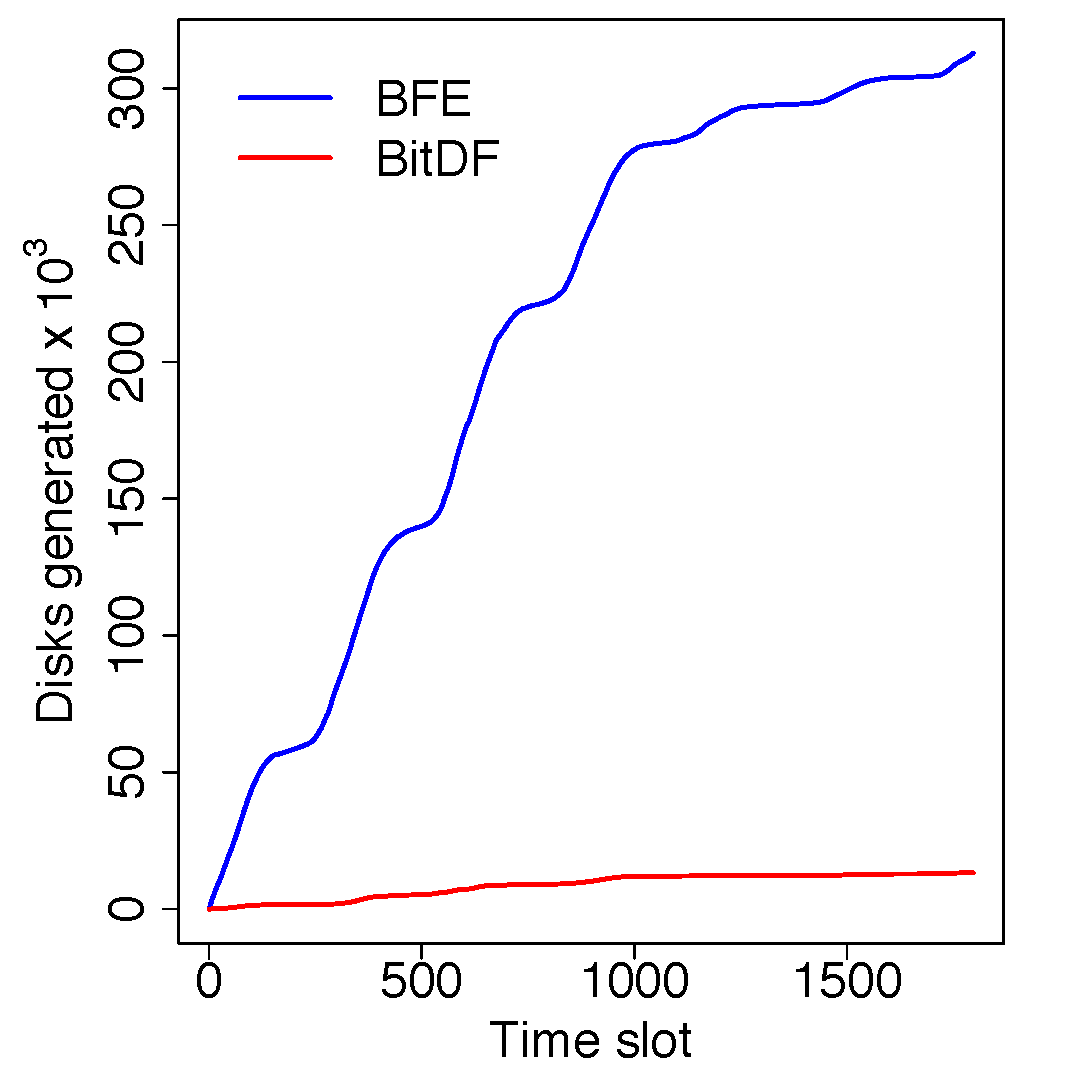
\includegraphics[width=\textwidth]{images/TDrive_d.eps}
        \label{fig:tdrive_disks}
    \end{subfigure}
    \footnotesize{Source: Made by the author.}
    \label{fig:tdrive_results2}
\end{figure*}

\section{Brinkhoff Dataset}
\label{sec:brinkhoff}
Likewise BerlinMOD, Brinkhoff is also a city traffic generation model \citep{brinkhoffpaper}. We generated a synthetic
dataset using the Minnesota Web-based Traffic Generator \citep{mntg}, having 2000 as the "Starting Vehicles" and 100 as
the "Simulation Time" parameters, which are the largest allowed numbers by the generator. The result dataset has 314,523
entries and 7000 unique $O_{id}$.

\begin{figure*}[h!]
    \centering
    \caption{Results varying $\delta$ and $\epsilon$ for Brinkhoff dataset}
    \begin{subfigure}[t]{0.48\textwidth}
        \caption{$\mu = 4$, $\epsilon = 200$ and $\delta$ varying}
        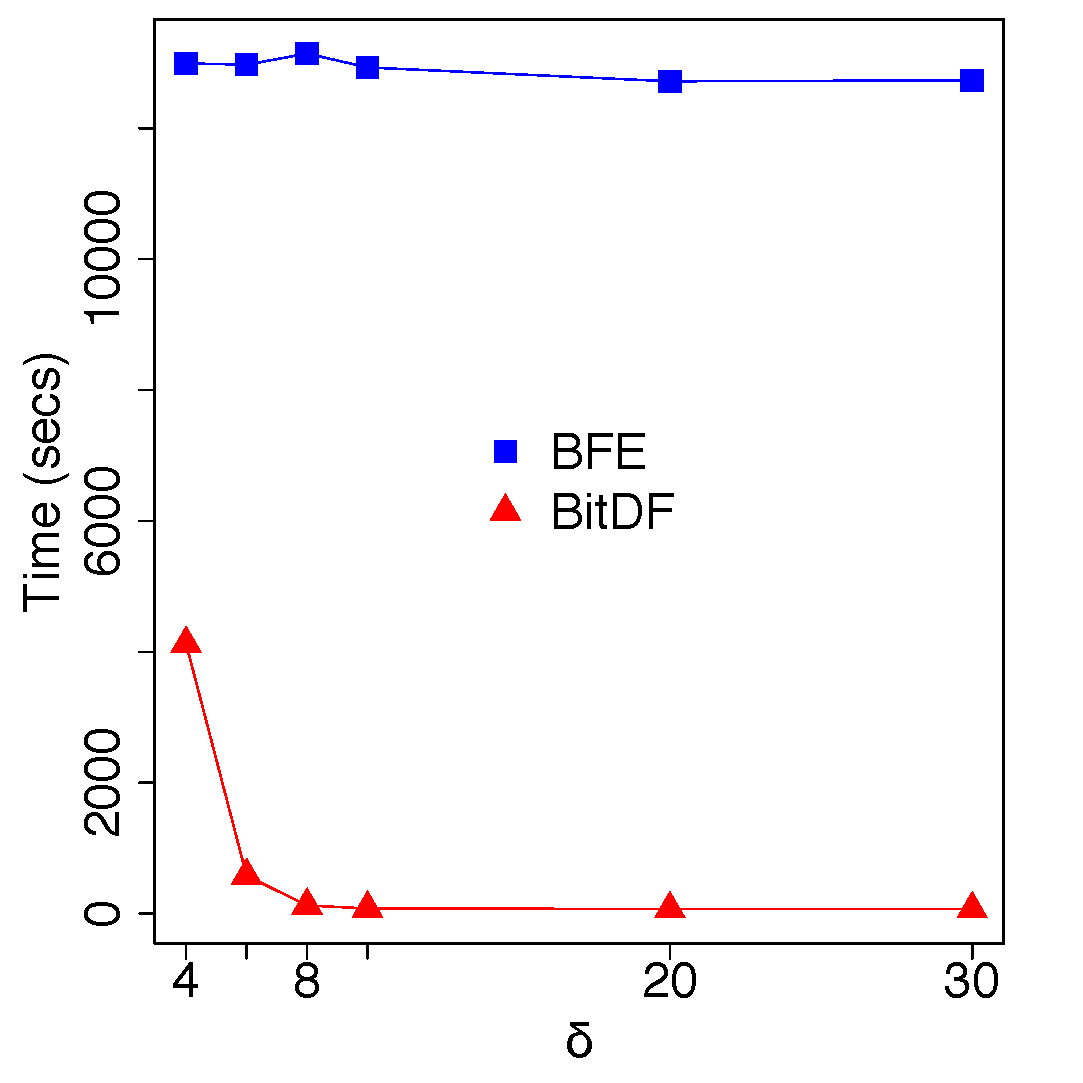
\includegraphics[width=\textwidth]{images/Brinkhoff_n_4_g_200_varying_l.eps}
        \label{fig:brinkhoff_vary_l}
    \end{subfigure}
    \begin{subfigure}[t]{0.48\textwidth}
        \caption{$\mu = 4$, $\delta = 8$ and $\epsilon$ varying}
        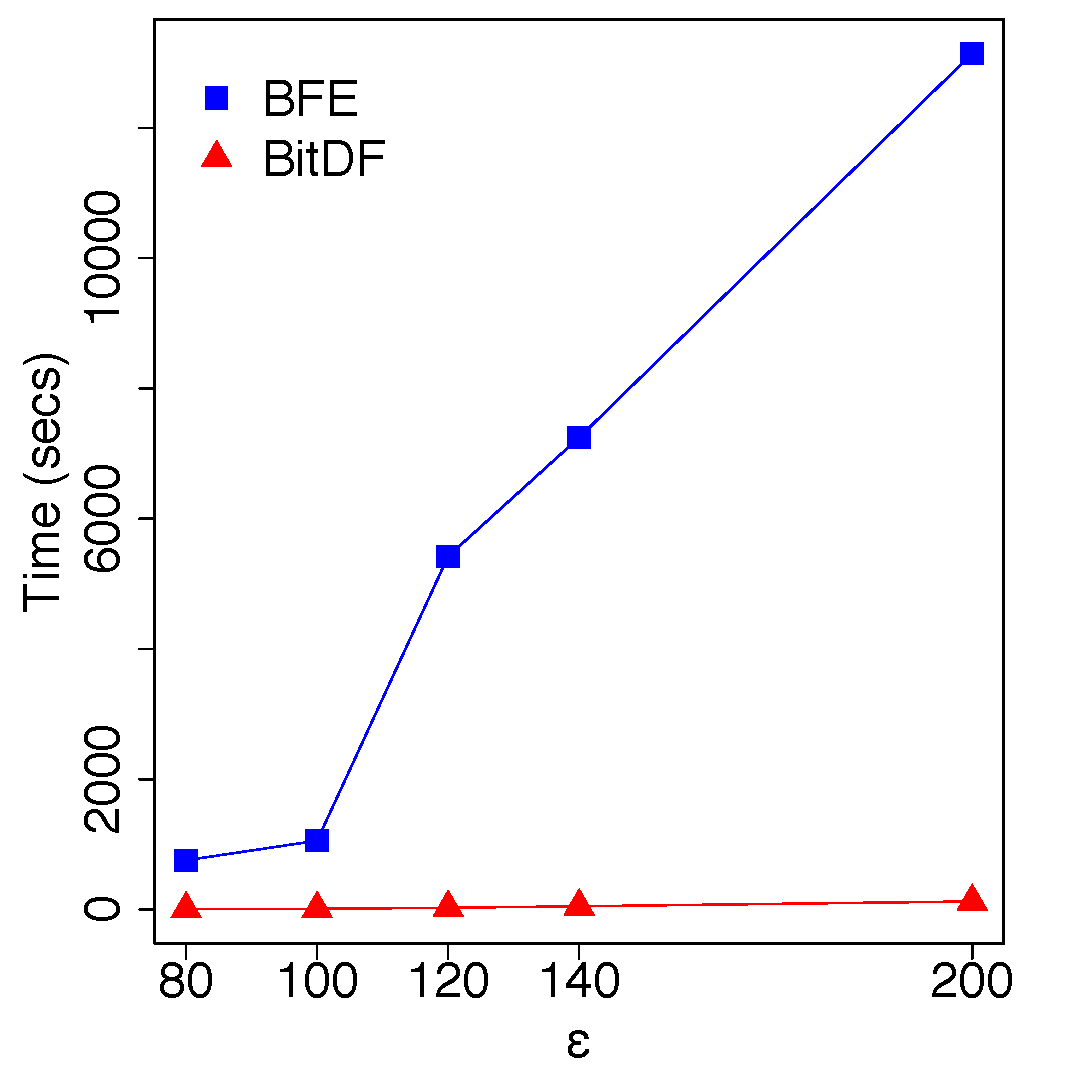
\includegraphics[width=\textwidth]{images/Brinkhoff_n_4_l_8_varying_g.eps}
        \label{fig:brinkhoff_vary_g}
    \end{subfigure}
    \footnotesize{Source: Made by the author.}
    \label{fig:brinkhoff_results}
\end{figure*}

\begin{figure*}[h!]
    \centering
    \caption{Results varying $\mu$ and number of disks generated over time for Brinkhoff dataset}
    \begin{subfigure}[t]{0.48\textwidth}
        \caption{$\delta = 8$, $\epsilon = 200$ and $\mu$ varying}
        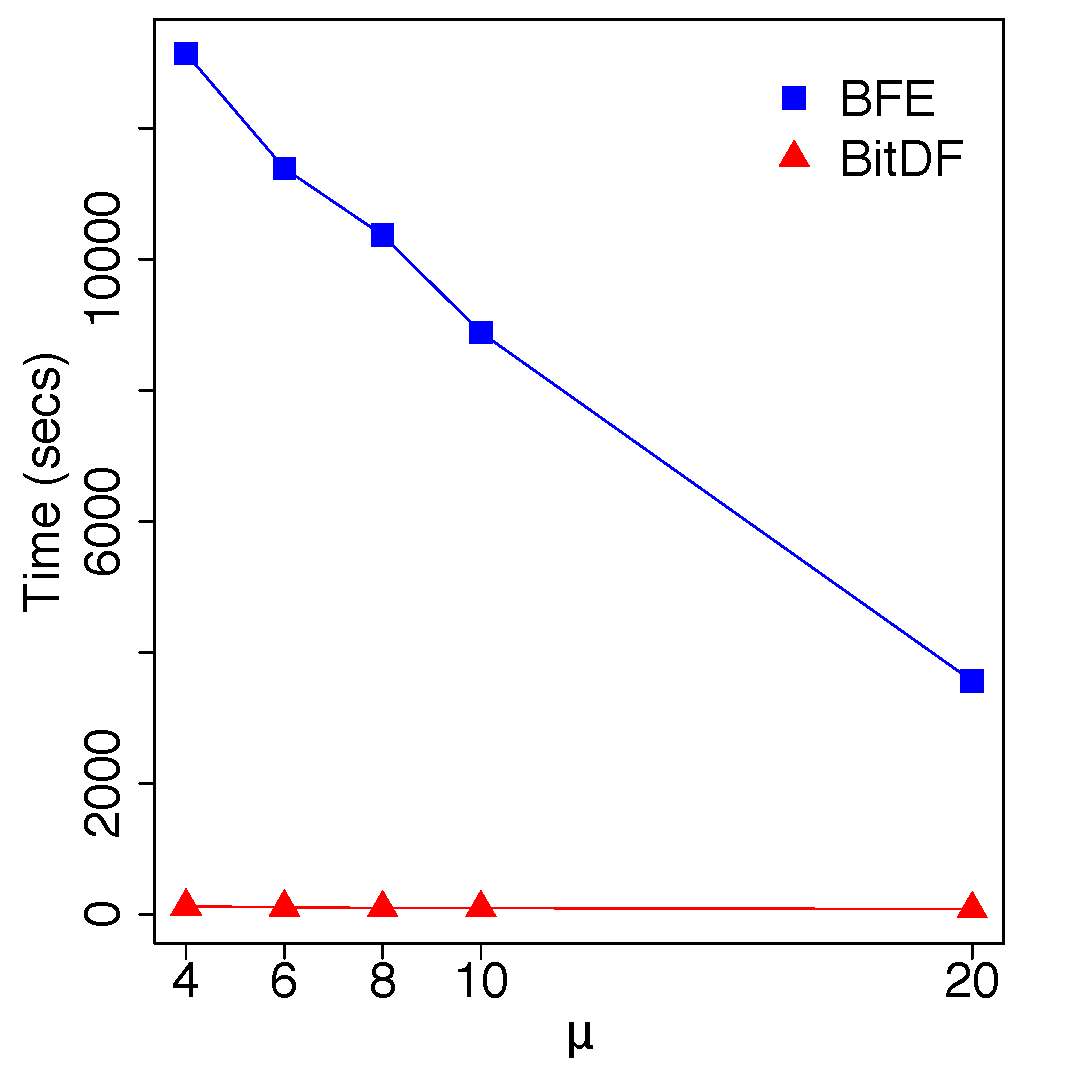
\includegraphics[width=\textwidth]{images/Brinkhoff_l_8_g_200_varying_n.eps}
        \label{fig:brinkhoff_vary_n}
    \end{subfigure}
    \begin{subfigure}[t]{0.48\textwidth}
        \caption{Cumulative disks by time}
        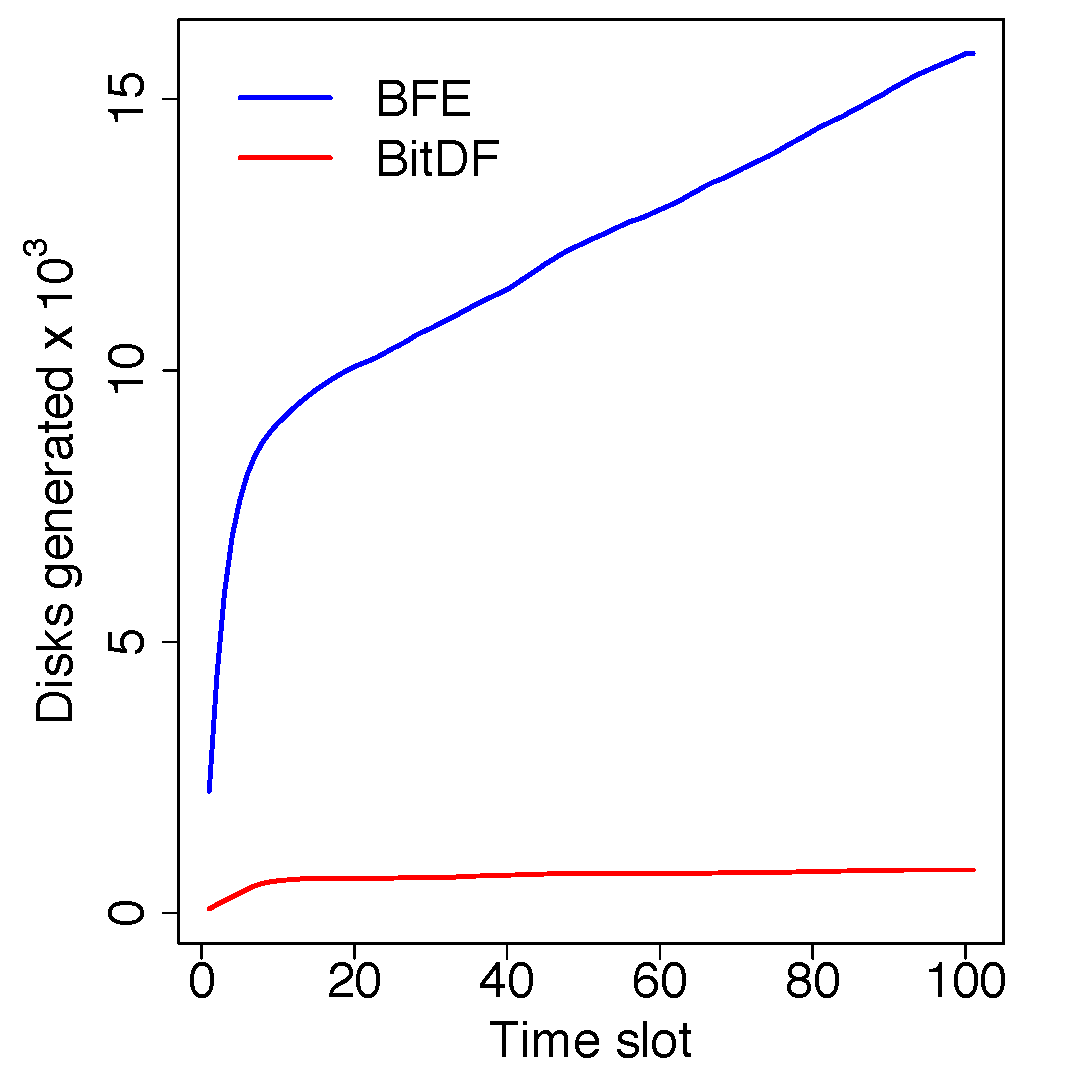
\includegraphics[width=\textwidth]{images/Brinkhoff_d.eps}
        \label{fig:brinkhoff_disks}
    \end{subfigure}
    \footnotesize{Source: Made by the author.}
    \label{fig:brinkhoff_results2}
\end{figure*}

The results achieved with this dataset were the best that \ac{bitdf} was able to get amongst the other datasets analyzed
in this dissertation, as one can notice by looking to \figref{fig:brinkhoff_results} and
\figref{fig:brinkhoff_results2}. There were huge drops in execution time, as depicted in \figref{fig:brinkhoff_vary_l},
where \ac{bitdf} analyzed the whole dataset in only 69 seconds, while \ac{bfe} took 12,732 seconds, representing an
improvement of 99.5\%. Another great running time improvement of 99\% can be seen when we varied the $\epsilon$
parameter, as shown in \figref{fig:brinkhoff_vary_g}, droping from 13,141 seconds to only 125 seconds. We can see in
\figref{fig:brinkhoff_vary_n} that even with the variation of $\mu$, \ac{bitdf} was able to show huge improvement, with
results ranging from 98\% to 99\% of \ac{cpu} time reduction. Additionally, we can see in \figref{fig:brinkhoff_disks}
that we were able to reduce the number of disks by 95\%, which is a dramatic improvement and is reflecting directly in
the running time improvements that we could see with this dataset.
\vfill

% Multi-thread evaluations
\section{Multi-threaded evaluation}
After implementing the architecture proposed in \secref{sec:architecture}, evaluating it in \chapref{chp:results} and
seeing great improvements in the running time when compared with other algorithms, we decided to test how our system
would perform by taking advantage of the multi-core paradigm that is been widely used nowadays. We then took a step
further and implement a new \ac{dp}, that we called \ac{pfp}. \ac{pfp} was implemented having in mind the \ac{mt} model
described in \secref{subsec:multithread}, which we call \ac{bitdf} \ac{mt}.

In order to see how \ac{bitdf} \ac{mt} would perform, we took from \chapref{chp:results} the worst performances of
\ac{bitdf} for each dataset and compared such performance against \ac{bitdf} \ac{mt} running with different number of
worker threads executing in parallel.

Our benchmarks were executed in a different machine from that one mentioned in the beginning of \chapref{chp:results},
in a way that we opted to get a better multi-core processor setup. With that in mind, we ran our experiments in a Linux
box, running Ubuntu 16.04 \ac{lts}, having an Intel Xeon \ac{cpu}, with 2.3 GHz and 4 physical cores, using Intel
Hyper-Threading technology \citep{hyper} meaning that we would theoretically have 8 different processing units.

Below we will present the benchmarks that were run for each dataset already seen in \chapref{chp:results}, namely
Trucks, TDrive, BerlinMOD and Brinkhoff. For each of the aforementioned datasets, we ran \ac{bitdf} \ac{mt} with the
same parameters as the longest \ac{bitdf} run presented in \chapref{chp:results}, varying the worker threads from 1
(pure \ac{bitdf}) to 30. With variations of 1 worker thread from 1 to 10, 2 worker threads from 10 to 20 and 5 worker
threads from 20 to 30. It is important to notice that when we say that we are running with $x$ worker threads, we are
actually running with $2*x$ threads: $x$ $c_t$ threads processing different \acp{egc} plus 1 $d_t$ thread (attached to
its $c_t$ thread) processing the disks generated by its parent $c_i$. We set the result of pure \ac{bitdf} as being
100\% of the total executing time and highlighted it with red color and all \ac{bitdf} \ac{mt} runs are in blue, always
being a percentage of the highlighted result. It is worth mentioning here that the only metric that we are evaluating in
these experiments is the running time of \ac{bitdf} \ac{mt}, because the number of generated disks will be the same that
we have seen in the previous results shown for \ac{bitdf} in \chapref{chp:results}, since we are still using the same
bitmap filtering heuristic proposed by \ac{bitdf}. Moreover, in order to have a better idea on how \ac{bitdf} \ac{mt}
outperforms \ac{bitdf} and \ac{bfe}, we show some graphs depicting the running time of them together, for each dataset.
For such comparion, we picked 5 and 7 as the number of worker threads for \ac{bitdf} \ac{mt}, since those are the values
that show the best peformance overall.

First we present the results for the Trucks dataset, which we ran with the following parameters (based on previous
results from \secref{sec:trucks}): $\mu=4$, $\delta=20$ and $\epsilon=1.5$. That dataset would be the most difficult one
to show running time improvements due to its small size and running times being already fast (with the longest one being
around 200 seconds for \ac{bitdf}). Despite that, we can see in \figref{fig:trucks_threads} that we were able to reduce
as much as 51\% when running with 5 $c_t$ threads, which totalizes 10 threads. After that we can see that we could stay
almost stable, not gaining any performance but also not deteriorating it too much. Such performance stabilization is an
expected result, as the processor would start to schedule and pause the execution of threads, because of having all its
resources busy, as the number of executing threads exceeds too much the number of available processing units (cores).

\begin{figure}[h!]
    \centering
    \caption{Execution time reduction by number of threads for the Trucks dataset}
    \centerline{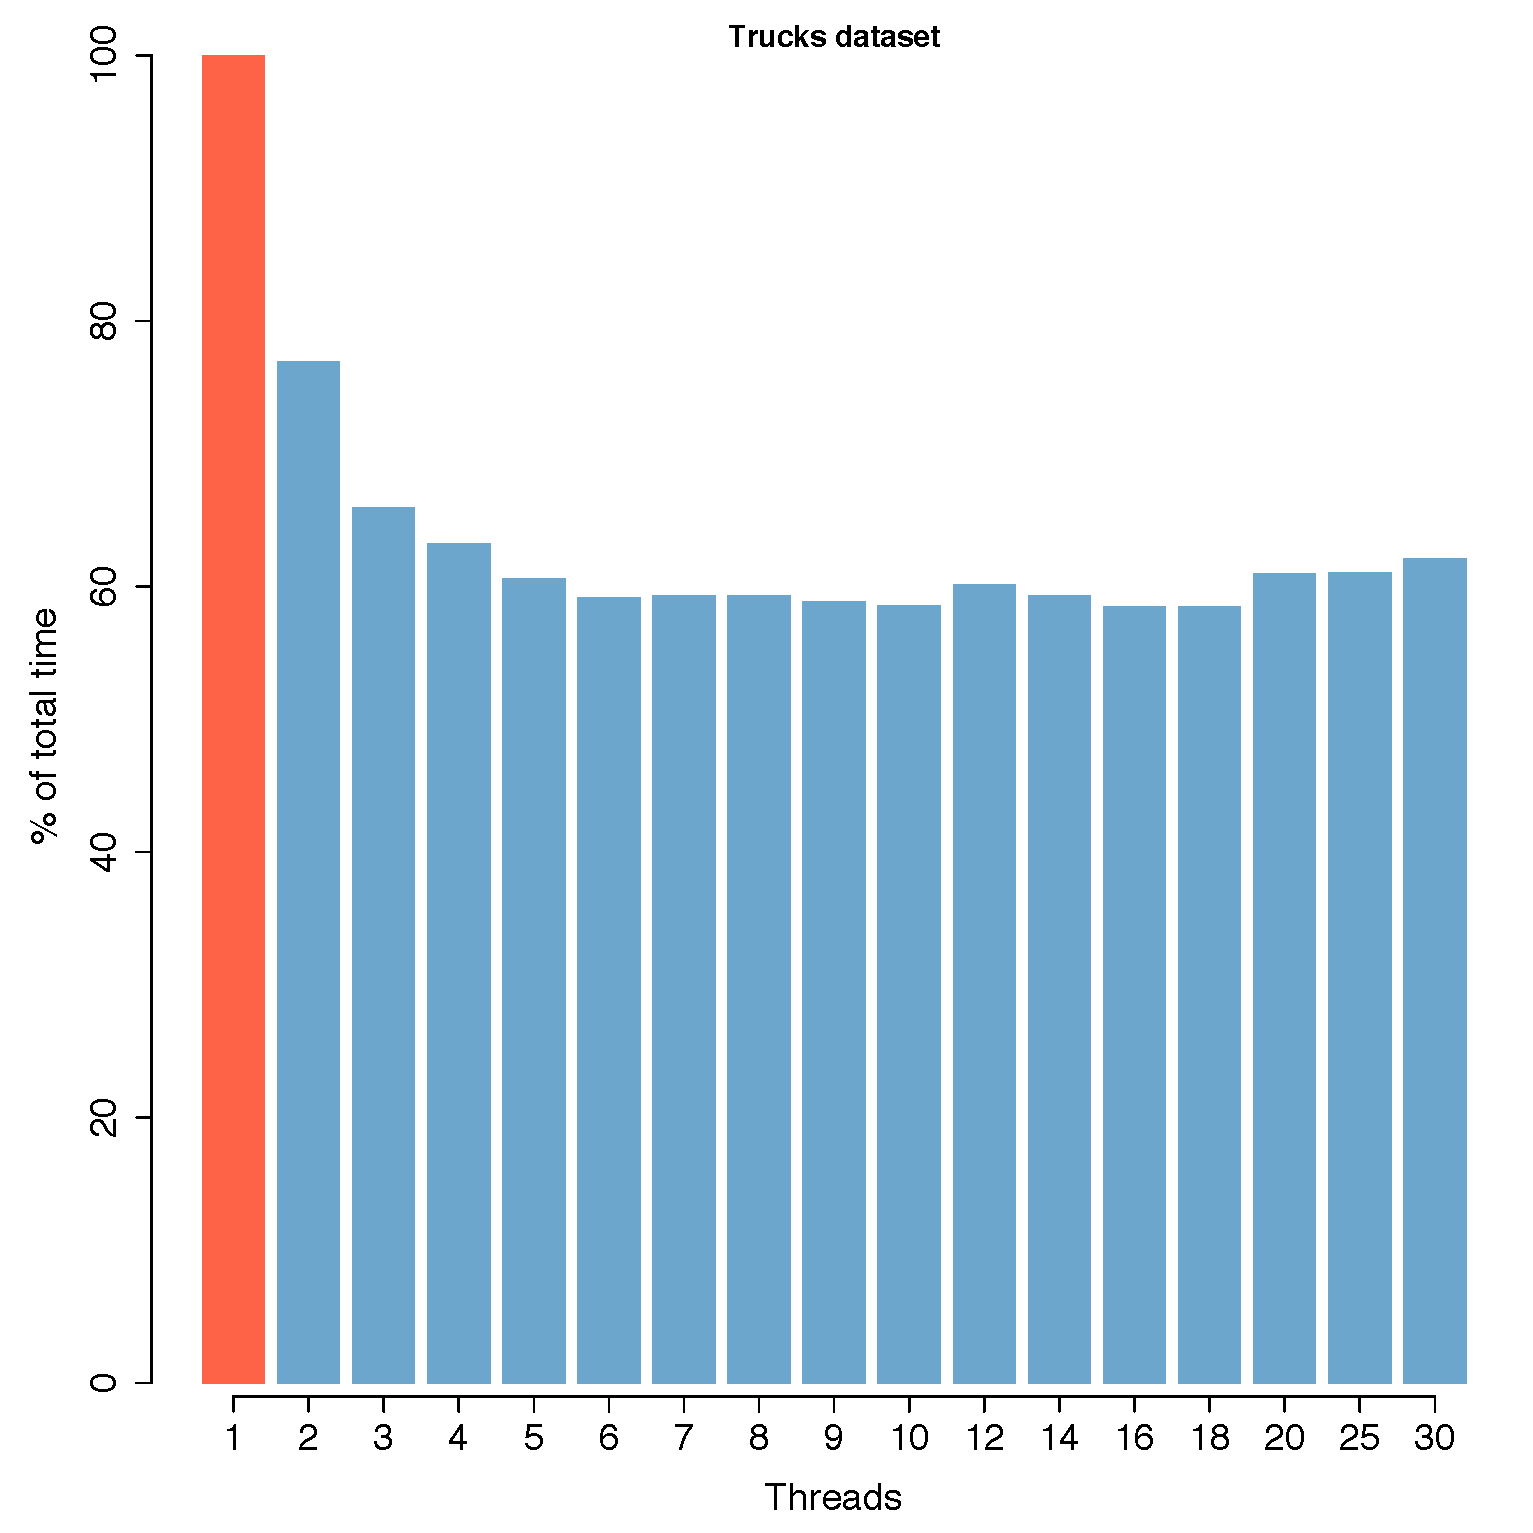
\includegraphics[width=0.7\textwidth]{images/Trucks_thread.eps}}
    \footnotesize{Source: Made by the author.}
    \label{fig:trucks_threads}
\end{figure}

\begin{figure*}[h!]
    \centering
    \caption{Results varying $\delta$ and $\epsilon$ for Trucks dataset}
    \begin{subfigure}[t]{0.49\textwidth}
        \caption{$\mu = 4$, $\epsilon = 1.5$ and $\delta$ varying}
        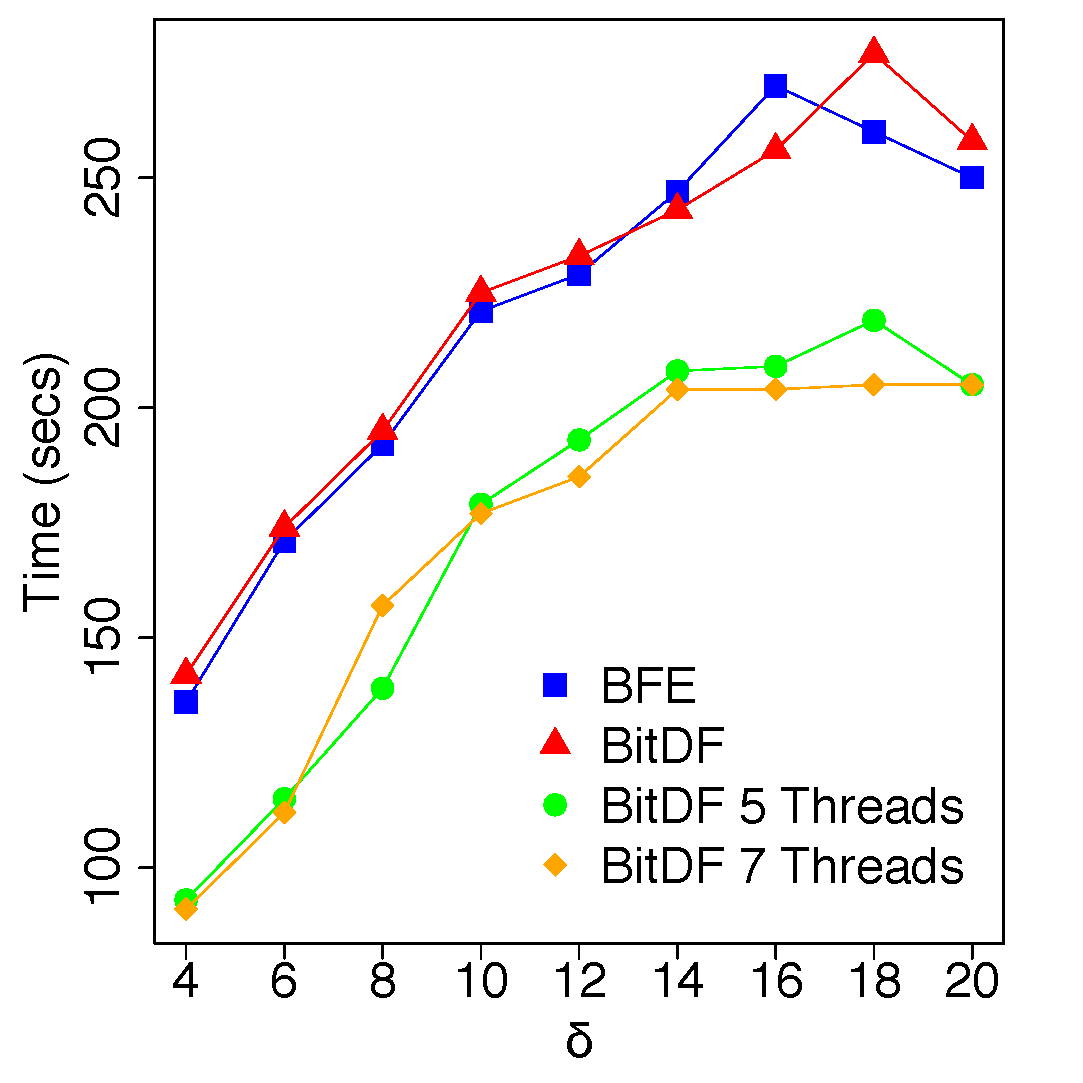
\includegraphics[width=\textwidth]{images/Trucks_complete_varying_l.eps}
        \label{fig:trucks_complete_vary_l}
    \end{subfigure}
    \begin{subfigure}[t]{0.49\textwidth}
        \caption{$\mu = 4$, $\delta = 20$ and $\epsilon$ varying}
        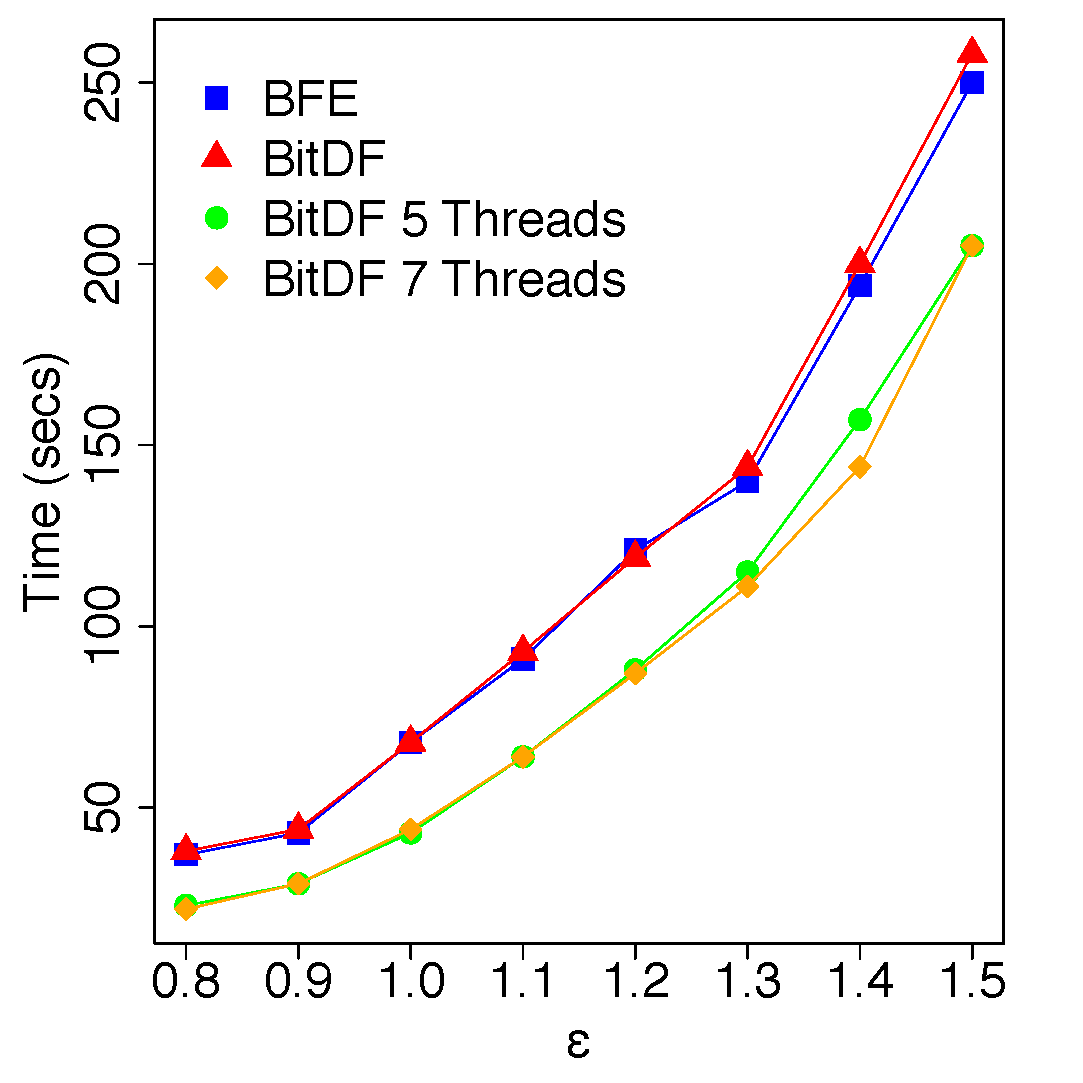
\includegraphics[width=\textwidth]{images/Trucks_complete_varying_g.eps}
        \label{fig:trucks_complete_vary_g}
    \end{subfigure}
    \footnotesize{Source: Made by the author.}
    \label{fig:trucks_complete_results}
\end{figure*}

\figref{fig:trucks_complete_results} and \figref{fig:trucks_complete_vary_n} show that we were able to achieve more
meaningful results with \ac{bitdf} \ac{mt}, than those presented in \secref{sec:trucks} and that the improvements
obtained with \ac{bitdf} \ac{mt} runing with both 5 and 7 worker threads were almost the same. We could reduce the
running time of \ac{bitdf} by 18\% when varying $\mu$ (\figref{fig:trucks_complete_vary_n}) and $\epsilon$
(\figref{fig:trucks_complete_vary_g}) and by 30\% when varying $\delta$ (\figref{fig:trucks_complete_vary_l}).

\begin{figure}[h!]
    \centering
    \caption{Results having $\delta = 20$, $\epsilon = 1.5$ and $\mu$ varying for the Trucks dataset}
    \centerline{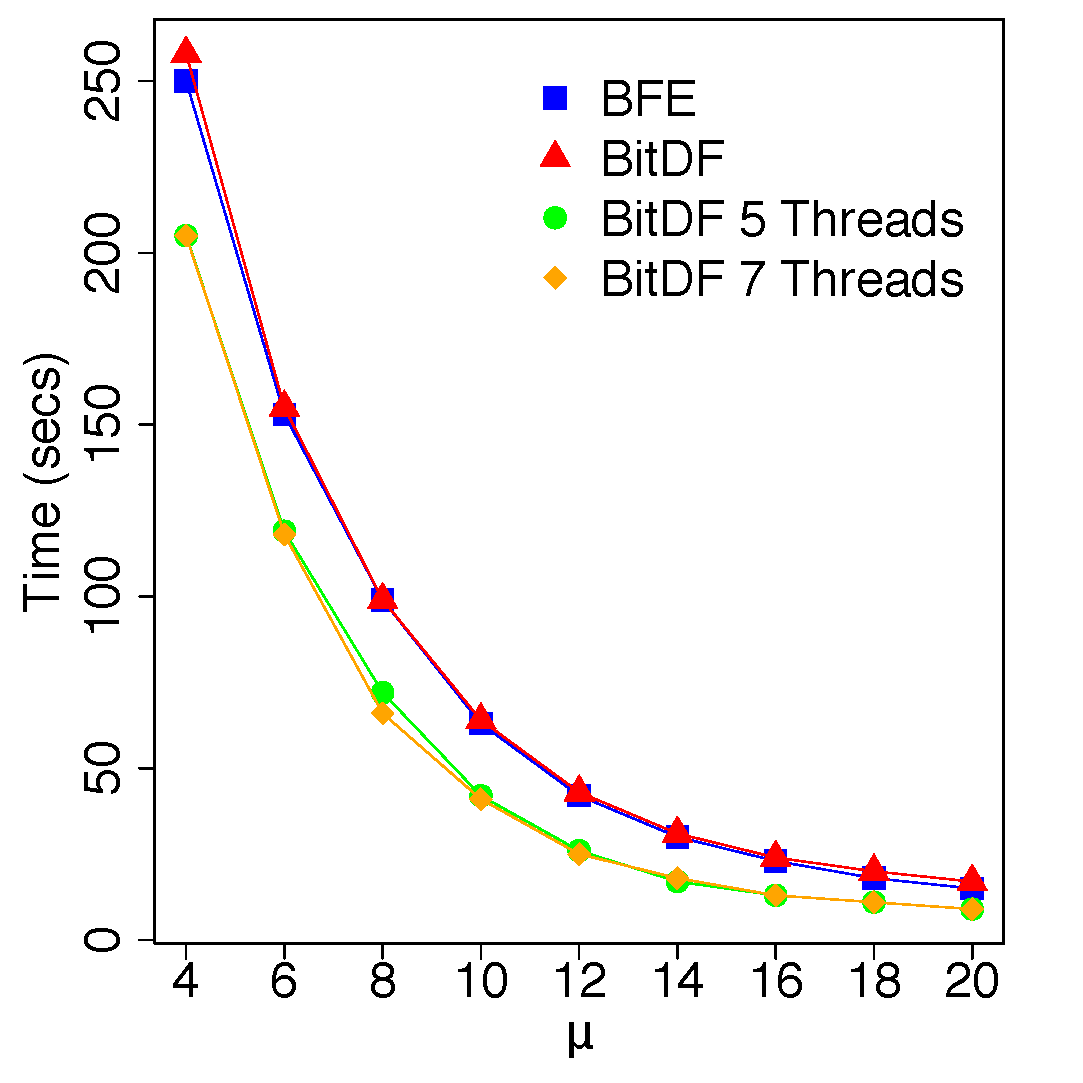
\includegraphics[width=0.5\textwidth]{images/Trucks_complete_varying_n.eps}}
    \footnotesize{Source: Made by the author.}
    \label{fig:trucks_complete_vary_n}
\end{figure}

In \figref{fig:berlinmod_threads}, we show the graph with the results for the BerlinMOD dataset. Due to its large size
and somewhat long execution times (as previously presented in \secref{sec:berlinmod}) we expected to obtain good results
in running \ac{bitdf} with independent worker threads. We have set our parameters to have the following values: $\mu=4$,
$\delta=8$ and $\epsilon=200$, as we had those resulting in the longest running time (around 1000 seconds) in our first
experiments with this dataset. It is noticed by \figref{fig:berlinmod_threads} that the results also tend to stabilize
when we reach 5 worker threads (10 in total), but we reach our best running time with 8 worker threads, with an
improvement of 62\%. It is also seen that the running time starts to get worse as we exceed the number of processing
units available (shown when \ac{bitdf} is executing with 30 worker threads, being 60 in total).

\begin{figure}[h!]
    \centering
    \caption{Execution time reduction by number of threads for the BerlinMOD dataset}
    \centerline{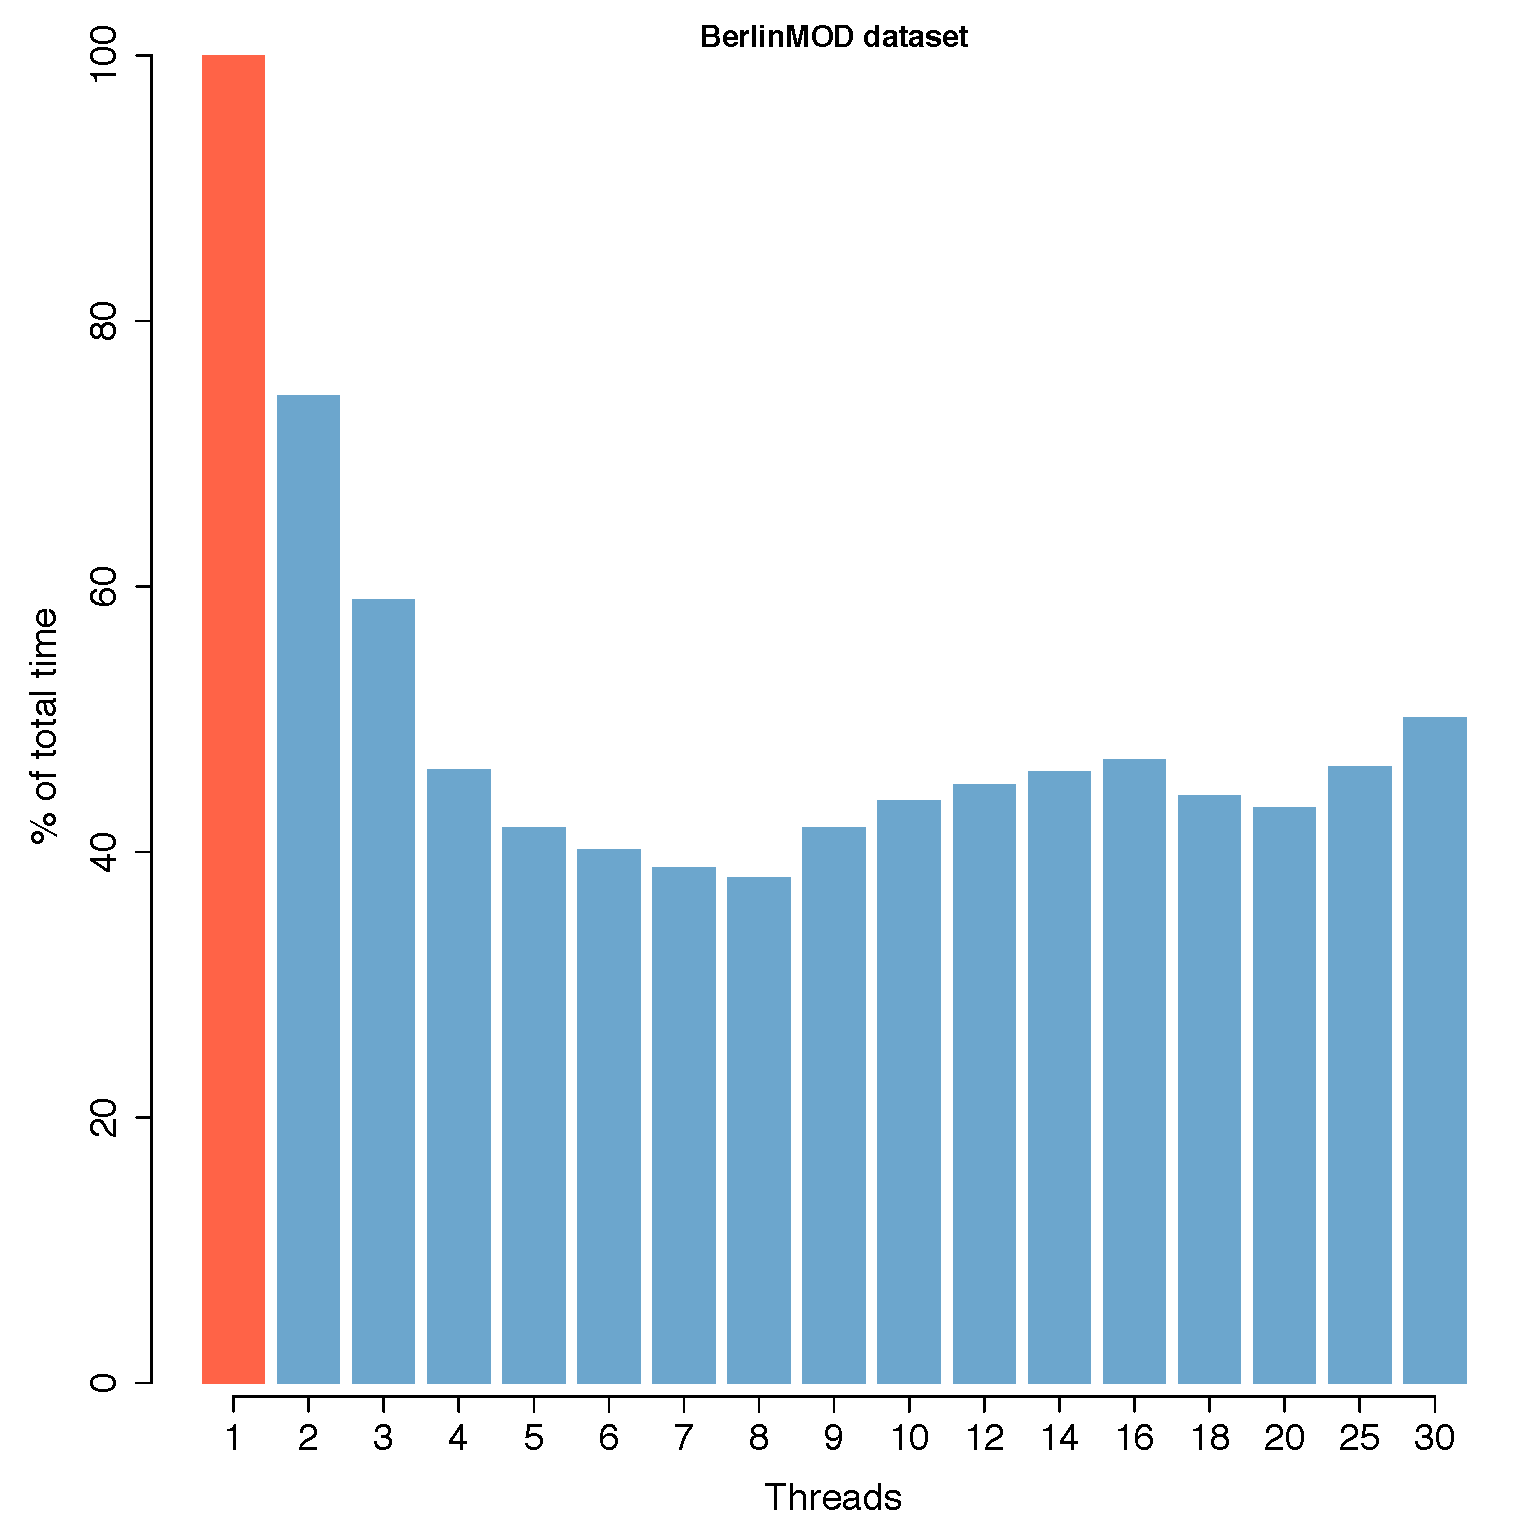
\includegraphics[width=0.7\textwidth]{images/BerlinMOD_thread.eps}}
    \footnotesize{Source: Made by the author.}
    \label{fig:berlinmod_threads}
\end{figure}

\begin{figure*}[h!]
    \centering
    \caption{Results varying $\delta$ and $\epsilon$ for BerlinMOD dataset}
    \begin{subfigure}[t]{0.49\textwidth}
        \caption{$\mu = 4$, $\epsilon = 100$ and $\delta$ varying}
        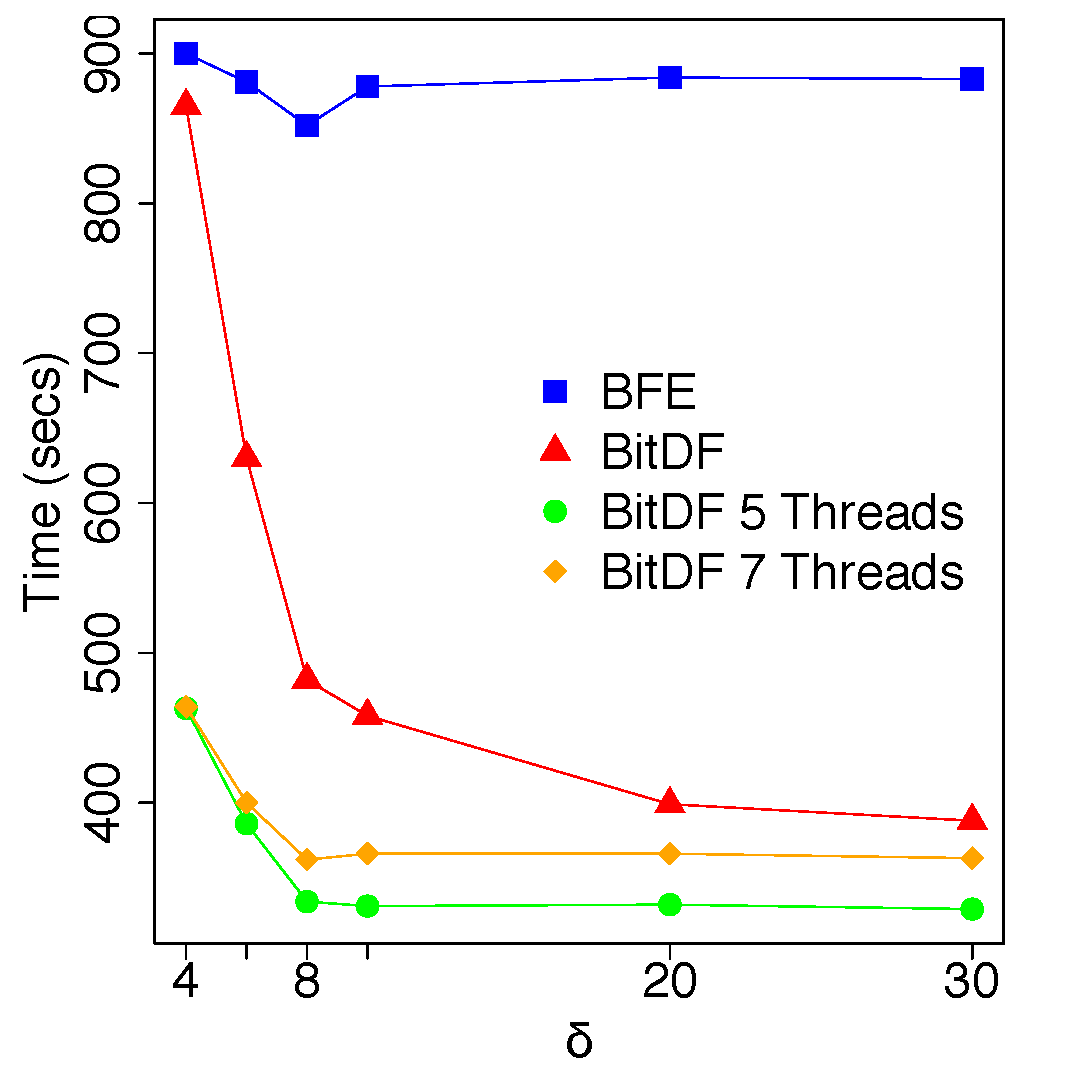
\includegraphics[width=\textwidth]{images/BerlinMOD_complete_varying_l.eps}
        \label{fig:berlinmod_complete_vary_l}
    \end{subfigure}
    \begin{subfigure}[t]{0.49\textwidth}
        \caption{$\mu = 4$, $\delta = 8$ and $\epsilon$ varying}
        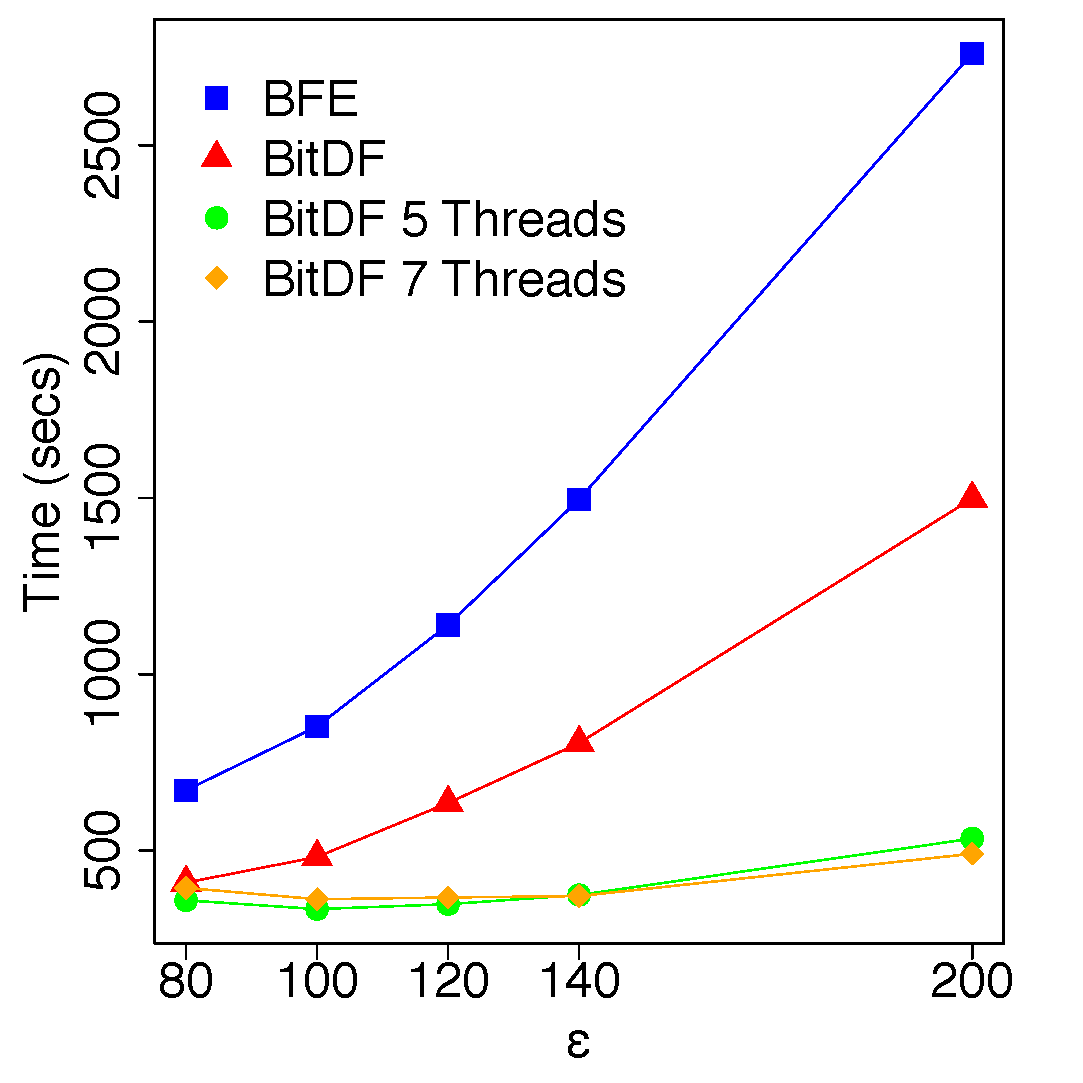
\includegraphics[width=\textwidth]{images/BerlinMOD_complete_varying_g.eps}
        \label{fig:berlinmod_complete_vary_g}
    \end{subfigure}
    \footnotesize{Source: Made by the author.}
    \label{fig:berlinmod_complete_results}
\end{figure*}

\begin{figure}[h!]
    \centering
    \caption{Results having $\delta = 8$, $\epsilon = 100$ and $\mu$ varying for the BerlinMOD dataset}
    \centerline{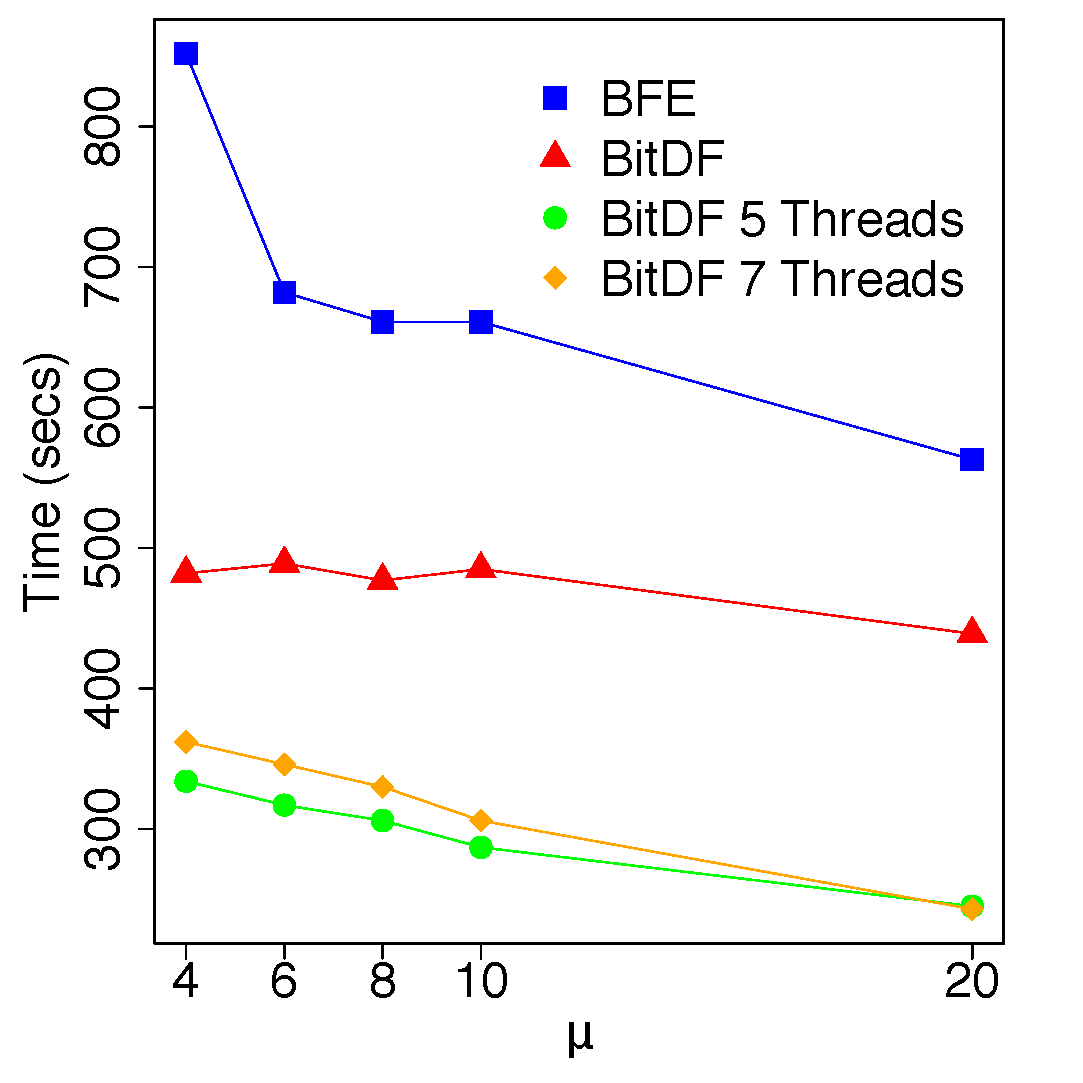
\includegraphics[width=0.5\textwidth]{images/BerlinMOD_complete_varying_n.eps}}
    \footnotesize{Source: Made by the author.}
    \label{fig:berlinmod_complete_vary_n}
\end{figure}

By looking at \figref{fig:berlinmod_complete_results} and \figref{fig:berlinmod_complete_vary_n}, one can see that even
where \ac{bitdf} had the worst results, \ac{bitdf} \ac{mt} was able to achieve important reductions in running time,
showing how a good multi-threaded remodeling is important in order to get the most out of a multi-core architecture.
\ac{bitdf} \ac{mt} improved the running time of \ac{bitdf} by 50\% when running with both 5 and 7 worker threads, as
shown in \figref{fig:berlinmod_complete_vary_l}. \ac{bitdf} \ac{mt} also achieved good results when we varied the $\mu$
parameter, having 45\% of running time decrease as it is depicted in \figref{fig:berlinmod_complete_vary_n}. Last, but
definitely not least, we can se in \figref{fig:berlinmod_complete_vary_g} that \ac{bitdf} \ac{mt} improved the running
time of \ac{bitdf} by 70\%, with both 5 and 7 worker threads.

\begin{figure}[h!]
    \centering
    \caption{Execution time reduction by number of threads for the TDrive dataset}
    \centerline{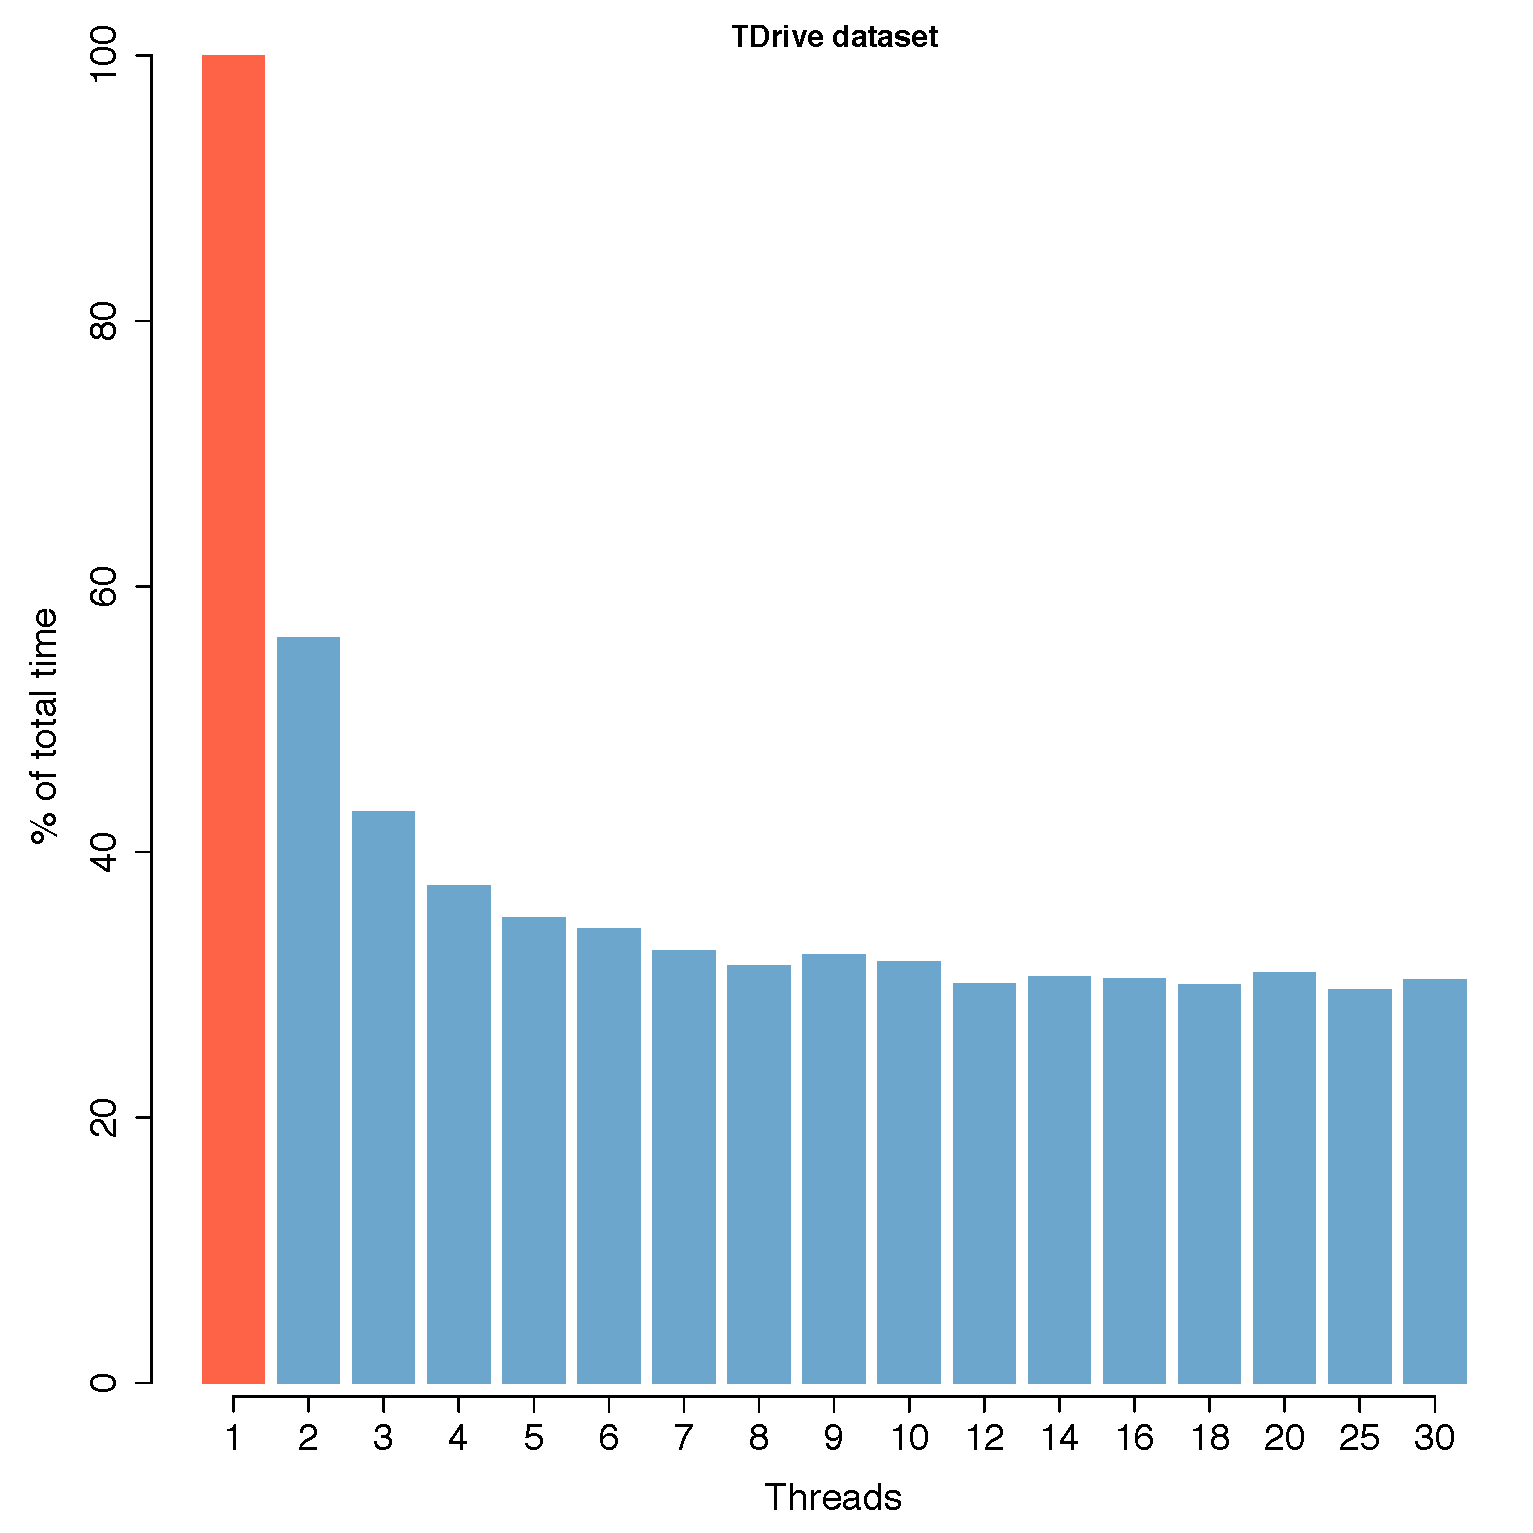
\includegraphics[width=0.7\textwidth]{images/TDrive_thread.eps}}
    \footnotesize{Source: Made by the author.}
    \label{fig:tdrive_threads}
\end{figure}

Another large dataset the we evaluate was the TDrive dataset, in which \ac{bitdf} showed great results when analzing it.
Based on the results presented in \secref{sec:tdrive}, we chose the parameter values that led to the longest executing
time (around 600 seconds): $\mu=4$, $\delta=4$ and $\epsilon=100$. \figref{fig:tdrive_threads} shows that the results
follow the same pattern that we have been seeing in the previous analyses: great improvements in the beginning, but
stabilizing as we exceed the number of processing units in the machine. We can also see some slight improvements even
when we evaluate with more than 5 worker threads. It is also depicted in \figref{fig:tdrive_threads} that we were able
to reduce the running time as much as 70\%, when compared to the single threaded model, which is a huge improvement
added to those already achieved in \secref{sec:tdrive}

\begin{figure*}[h!]
    \centering
    \caption{Results varying $\delta$ and $\epsilon$ for TDrive dataset}
    \begin{subfigure}[t]{0.49\textwidth}
        \caption{$\mu = 4$, $\epsilon = 100$ and $\delta$ varying}
        \includegraphics[width=\textwidth]{images/TDrive_complete_varying_l.eps}
        \label{fig:tdrive_complete_vary_l}
    \end{subfigure}
    \begin{subfigure}[t]{0.49\textwidth}
        \caption{$\mu = 4$, $\delta = 8$ and $\epsilon$ varying}
        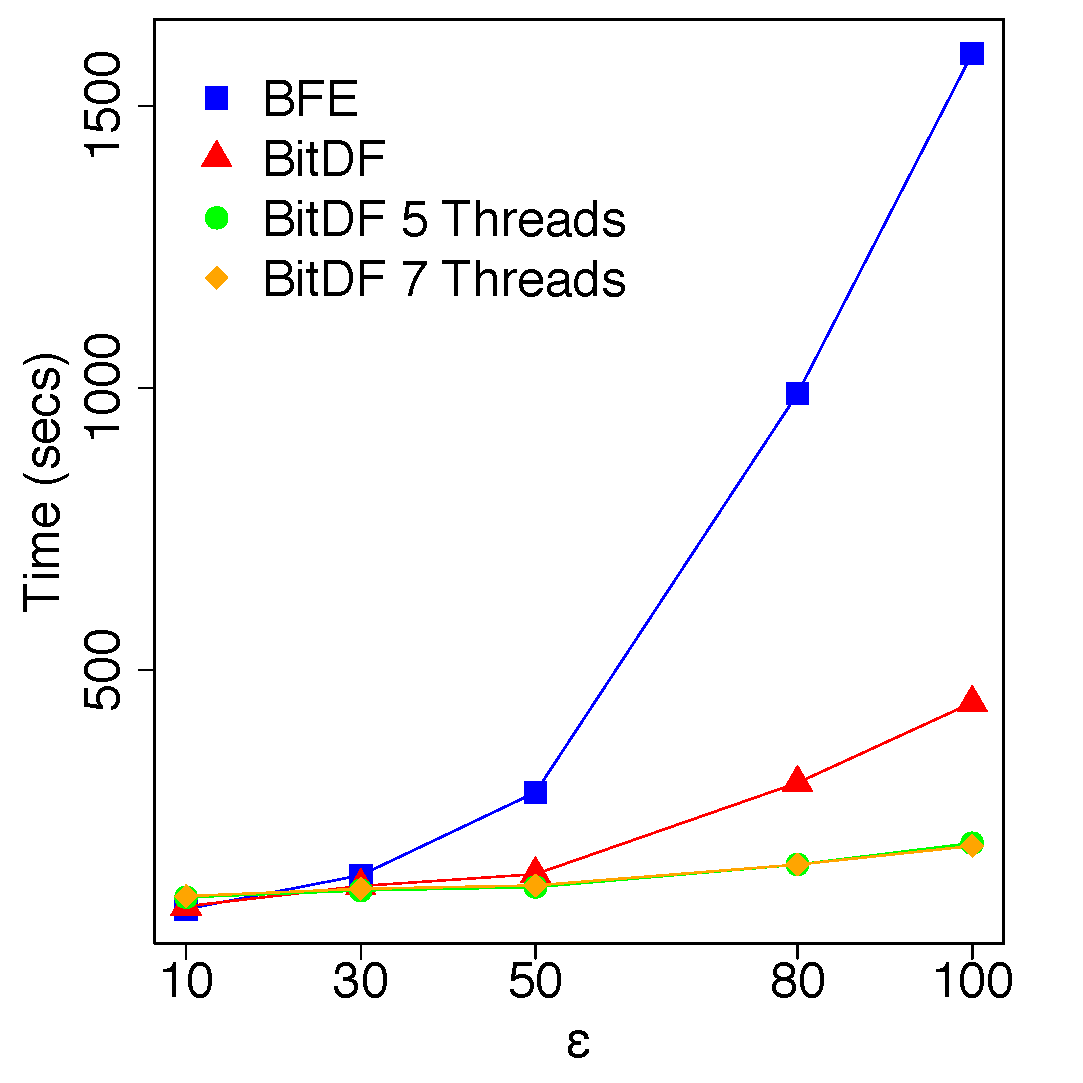
\includegraphics[width=\textwidth]{images/TDrive_complete_varying_g.eps}
        \label{fig:tdrive_complete_vary_g}
    \end{subfigure}
    \footnotesize{Source: Made by the author.}
    \label{fig:tdrive_complete_results}
\end{figure*}

\begin{figure}[h!]
    \centering
    \caption{Results having $\delta = 8$, $\epsilon = 100$ and $\mu$ varying for the TDrive dataset}
    \centerline{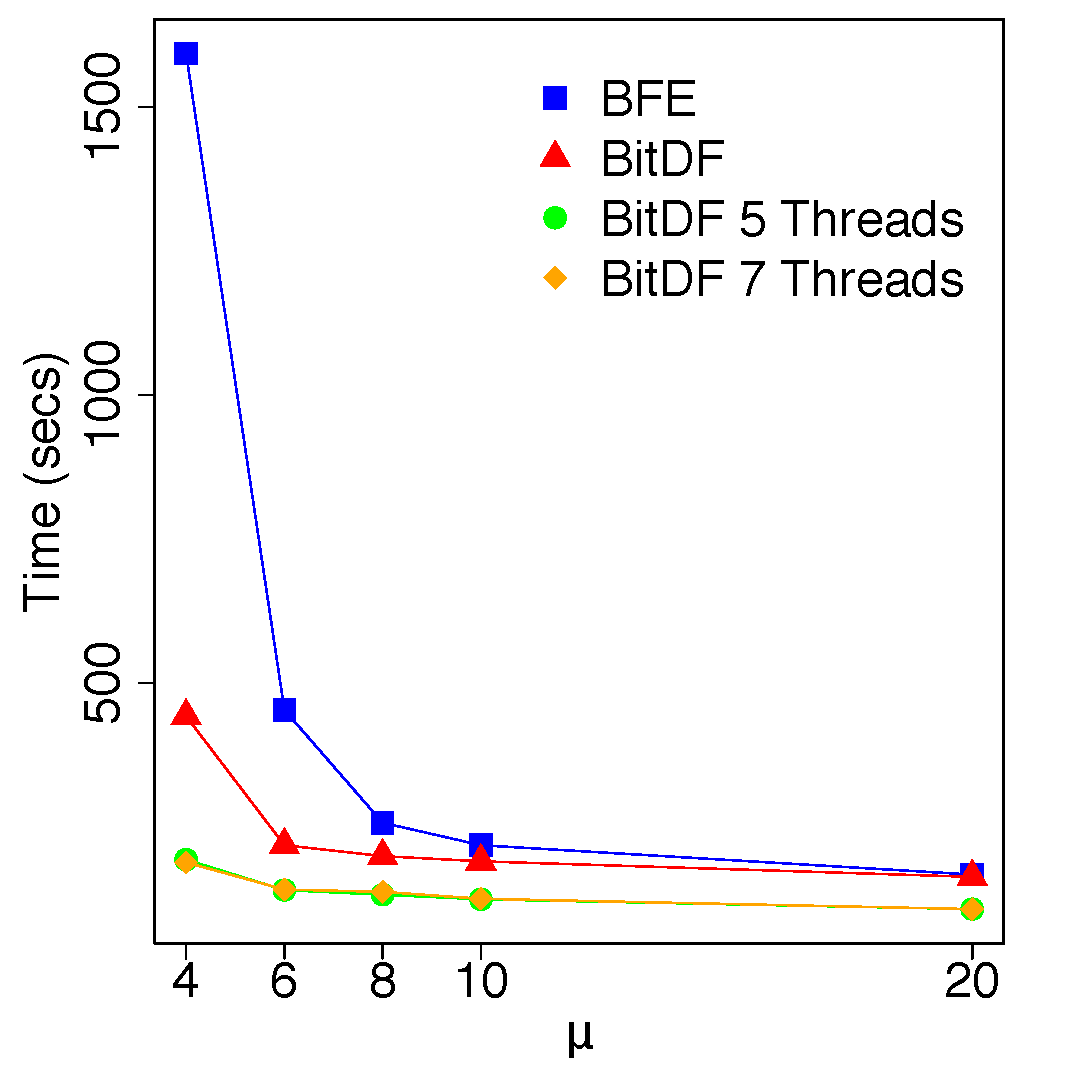
\includegraphics[width=0.5\textwidth]{images/TDrive_complete_varying_n.eps}}
    \footnotesize{Source: Made by the author.}
    \label{fig:tdrive_complete_vary_n}
\end{figure}

When it comes to comparing the running time of \ac{bitdf} \ac{mt} against \ac{bitdf} and \ac{bfe}, we can see that
\ac{bitdf} \ac{mt} was able to improve the running time even more than we have seen in \secref{sec:tdrive}. When varying
the parameter $\mu$ we could reduce the execution time by 60\%, as one can see in \figref{fig:tdrive_complete_vary_n}.
\figref{fig:tdrive_complete_vary_g} also shows improvements of 60\%, when compared against \ac{bitdf}, when varying the
parameter $\epsilon$. The best result though is when we varied the parameter $\delta$, in which we could improve the
\ac{bitdf} running time by 70\% when executing \ac{bitdf} \ac{mt} with both 5 and 7 worker threads, as depicted in
\figref{fig:tdrive_complete_vary_l}.

\begin{figure}[h!]
    \centering
    \caption{Execution time reduction by number of threads for the Brinkhof dataset}
    \centerline{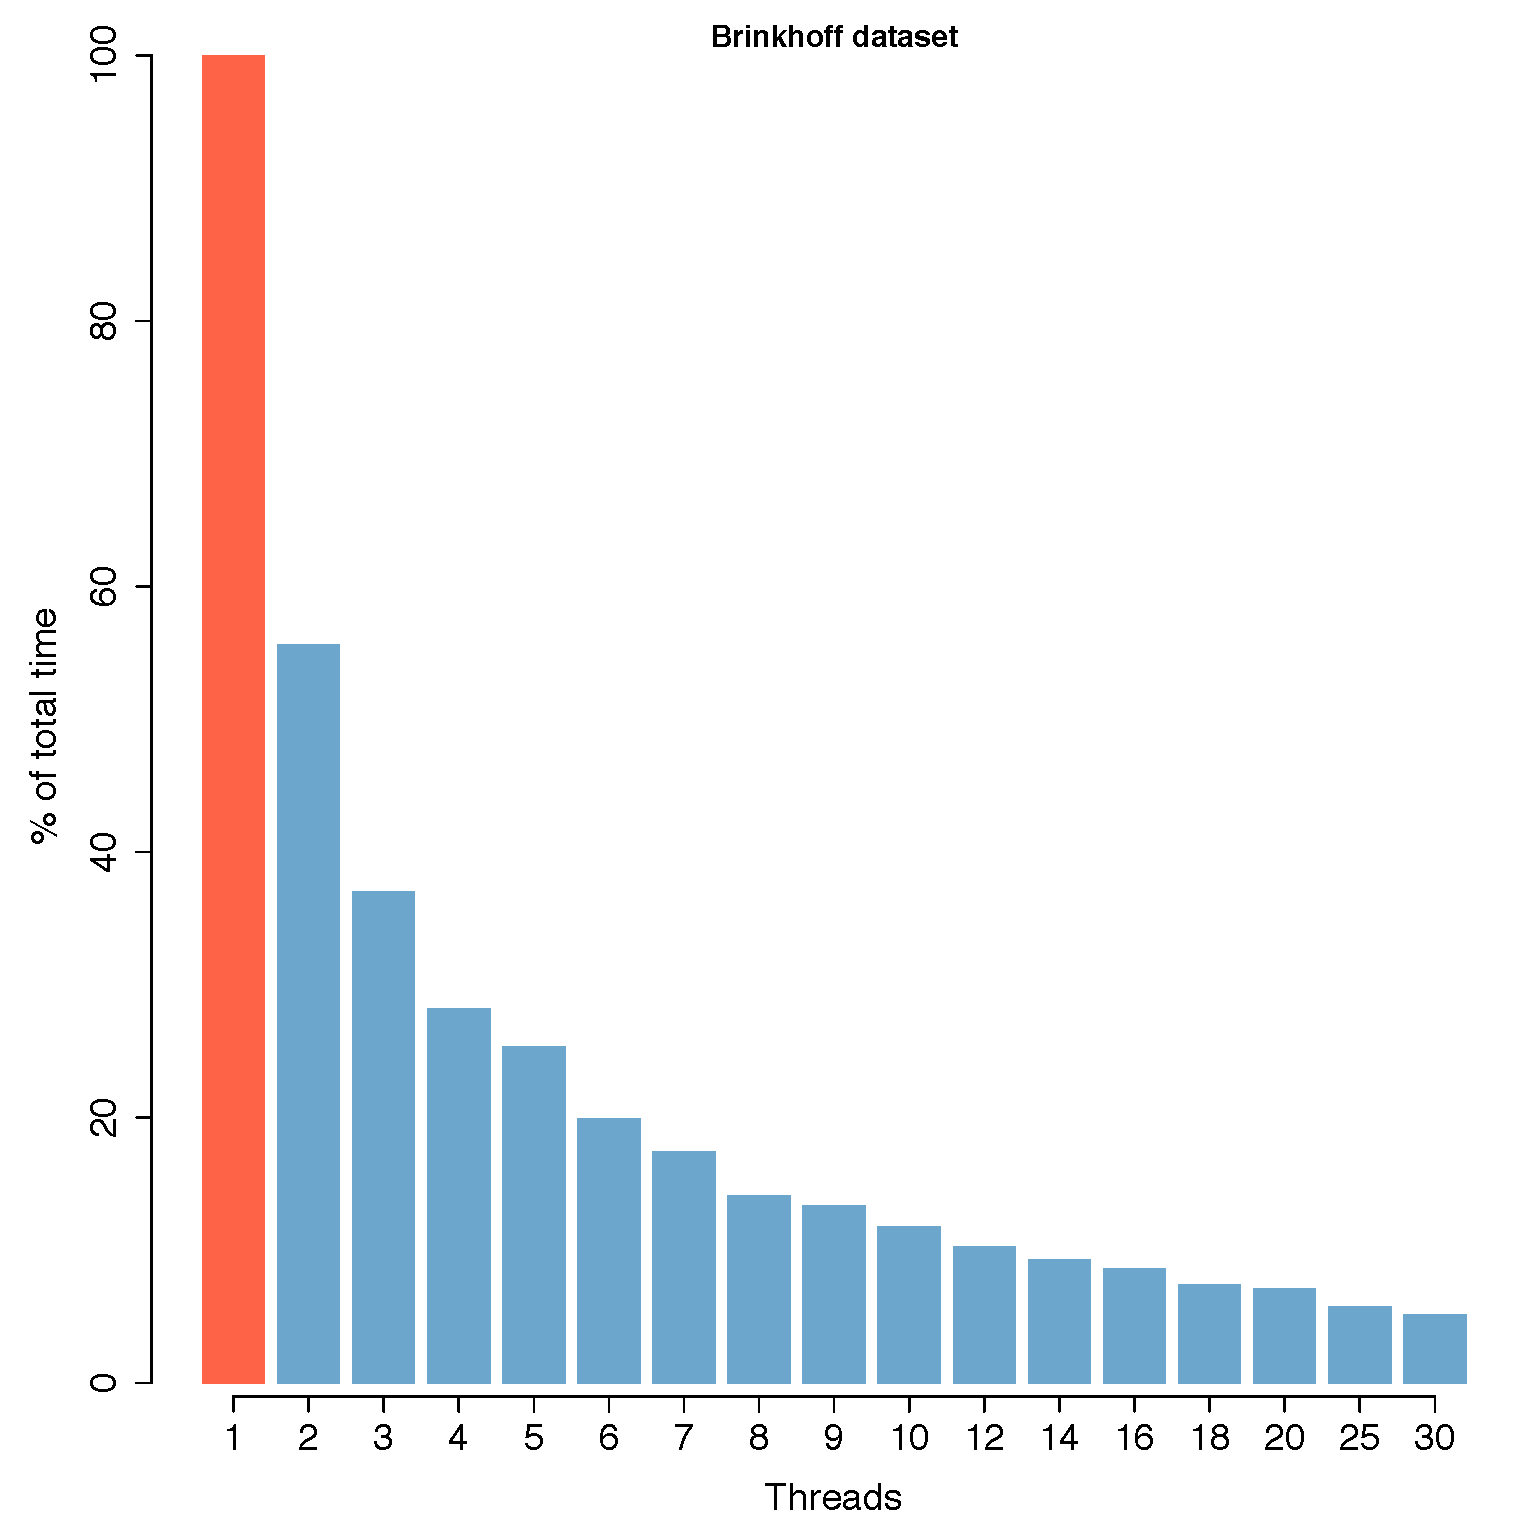
\includegraphics[width=0.7\textwidth]{images/Brinkhoff_thread.eps}}
    \footnotesize{Source: Made by the author.}
    \label{fig:brinkhoff_threads}
\end{figure}

Our last dataset to evaluate is the Brinkhoff synthetic dataset. We were already able to achieve huge running time
improvements with \ac{bitdf}, but we could achieve even more with \ac{bitdf} \ac{mt}. Based on the dataset results
(\secref{sec:brinkhoff}), we chose the running parameters as follows: $\mu=4$, $\delta=4$ and $\epsilon=1200$.
\figref{fig:brinkhoff_threads} shows that we were always able to reduce the \ac{bitdf} running time even with the number
of worker threads being way higher than the number of available processing units in the machine. That is a result that
is completely different from those that we saw with the previous datasets. Compared with the \ac{bitdf} run, we could
reduce the running time by 96\%, being that highest cutback achieved with 30 worker threads (60 in total). Given that
different behavior from the other datasets, we took a closer look on it when running with a high number of threads, in
order to try to find out the reason that \ac{bitdf} \ac{mt} runs better as the number of worker threads grow. As one can
see in \figref{fig:brinkhoff_disks_threads}, the number of disks that are being generated by the disk threads ($d_i$)
are very close to the final number of disks that are being inserted in the global disk set. That means that the each
disk thread is able to eliminate a lot of repeated and superset disks before returning them to be merged in the global
set. Another thing that is important to note is that the number of disks being generated is really small as time
advances, meaning that the points are more scattered over time, causing less disks to be generated and then less
synchronization between shared queues for each executing thread. Because of that, threads could spend less time blocked
waiting for shared data to become available.

\begin{figure}[h!]
    \centering
    \caption{Sum of disks generated by the disk threads (red) and number of disks that were inserted in the global disk
        set after subset/superset check (blue), by time slot}
    \centerline{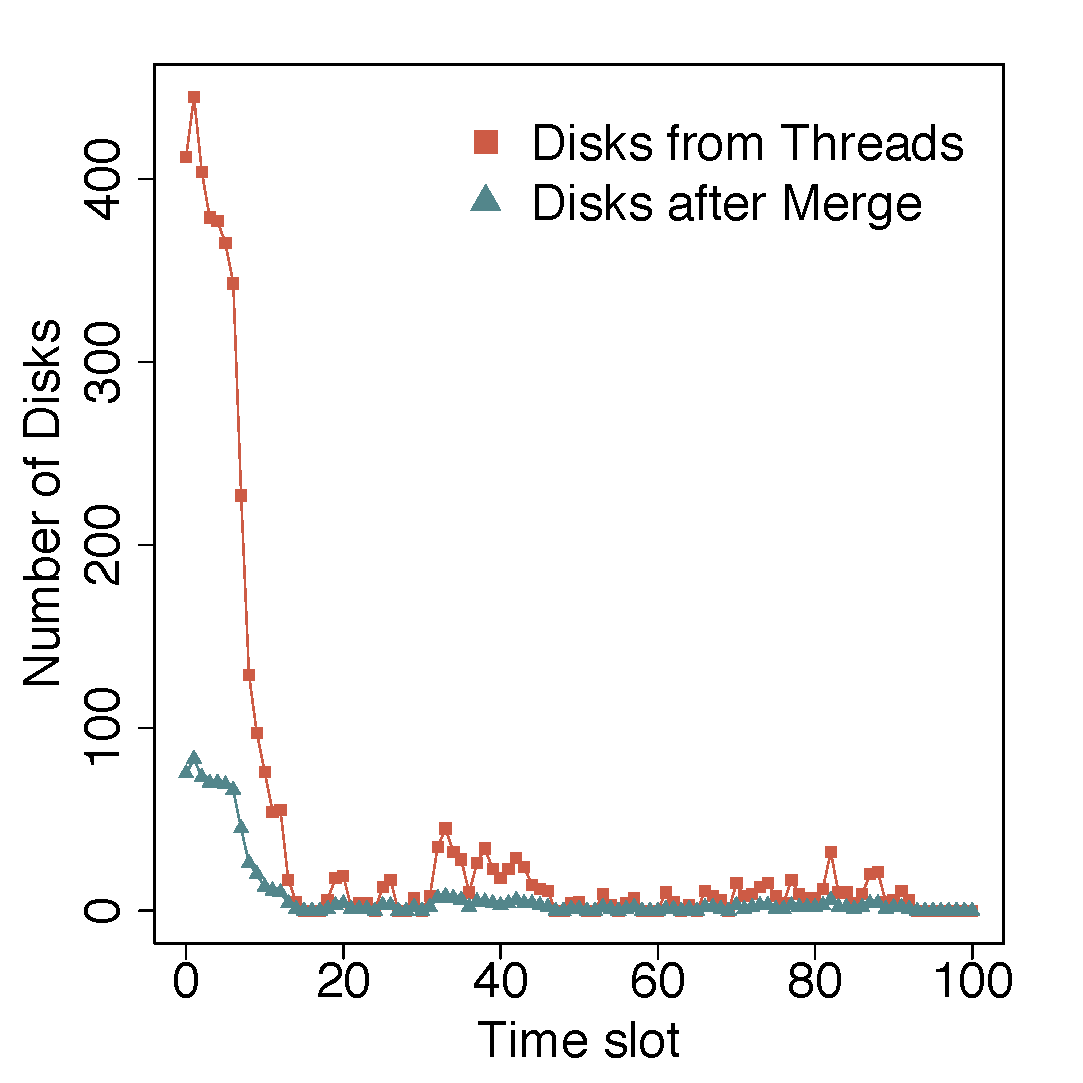
\includegraphics[width=0.7\textwidth]{images/Brinkhoff_disks_threads.eps}}
    \footnotesize{Source: Made by the author.}
    \label{fig:brinkhoff_disks_threads}
\end{figure}

Despite the reduction in running time of more than 90\% that \ac{bitdf} was able to achieve, as seen in
\secref{sec:brinkhoff}, we could reduce that number even more with \ac{bitdf} \ac{mt}. It is difficult to see the actual
difference between the running time of \ac{bitdf} and \ac{bitdf} \ac{mt}, due to the slowness of \ac{bfe} in that
dataset, which is causing the y axis range to be very large. However, \ac{bitdf} \ac{mt} with 5 and 7 worker threads
could reduce the time of \ac{bitdf} by 82\% when varying the $\mu$ parameters, as shown in
\figref{fig:brinkhoff_complete_vary_n}. When varying the $\epsilon$ parameter, \ac{bitdf} \ac{mt} with 5 and 7 worker
threads could also decrease the \ac{bitdf} running time by 82\% (\figref{fig:brinkhoff_complete_vary_g}). Finally, by
varying the $\delta$ parameter and running with 5 worker threads, \ac{bitdf} \ac{mt} could outperform \ac{bitdf} by
76\%, whereas by running with 7 worker threads, \ac{bitdf} \ac{mt} could be better by 85\%, as we can see in
\figref{fig:brinkhoff_complete_vary_l}.

\begin{figure*}[h!]
    \centering
    \caption{Results varying $\delta$ and $\epsilon$ for Brinkhoff dataset}
    \begin{subfigure}[t]{0.49\textwidth}
        \caption{$\mu = 4$, $\epsilon = 100$ and $\delta$ varying}
        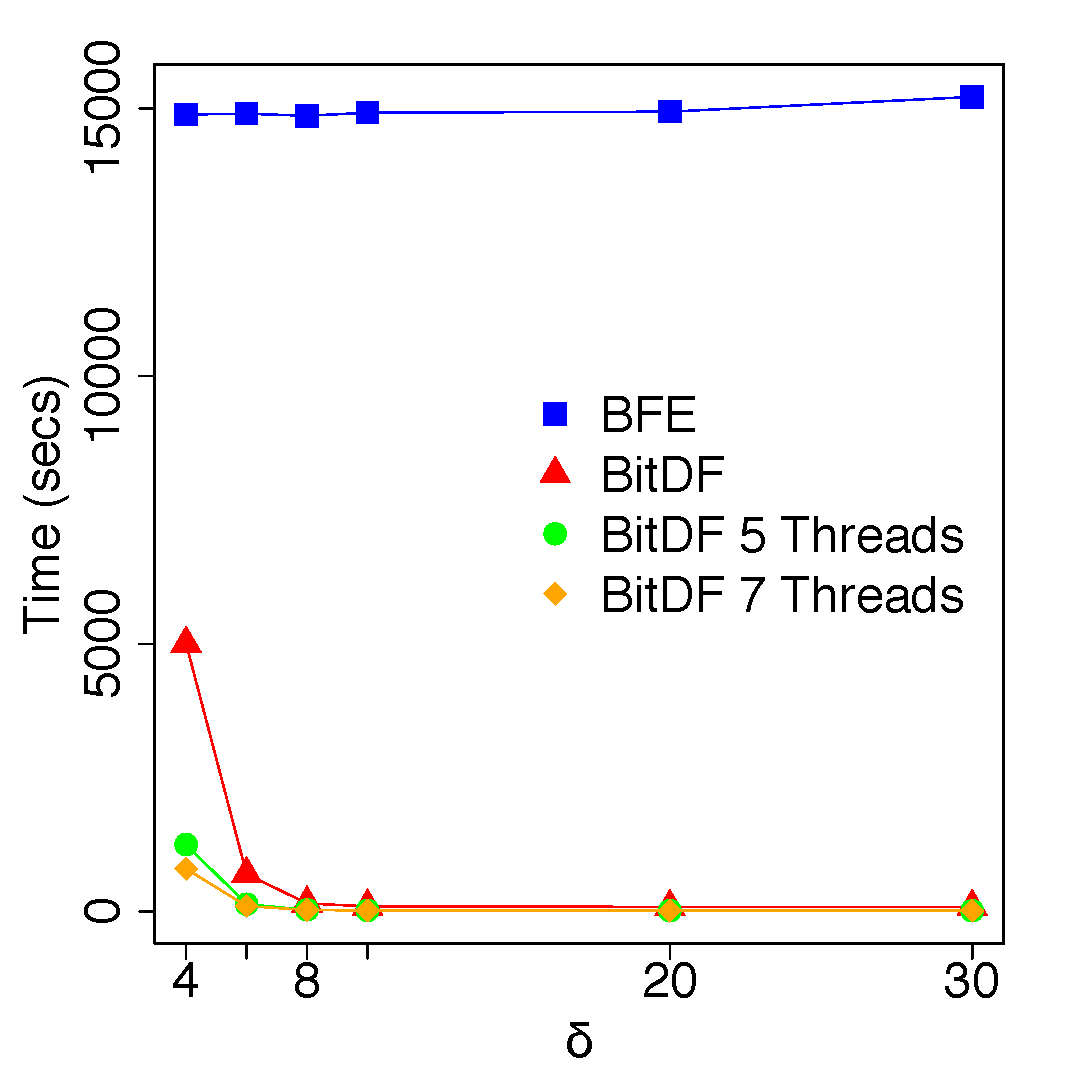
\includegraphics[width=\textwidth]{images/Brinkhoff_complete_varying_l.eps}
        \label{fig:brinkhoff_complete_vary_l}
    \end{subfigure}
    \begin{subfigure}[t]{0.49\textwidth}
        \caption{$\mu = 4$, $\delta = 8$ and $\epsilon$ varying}
        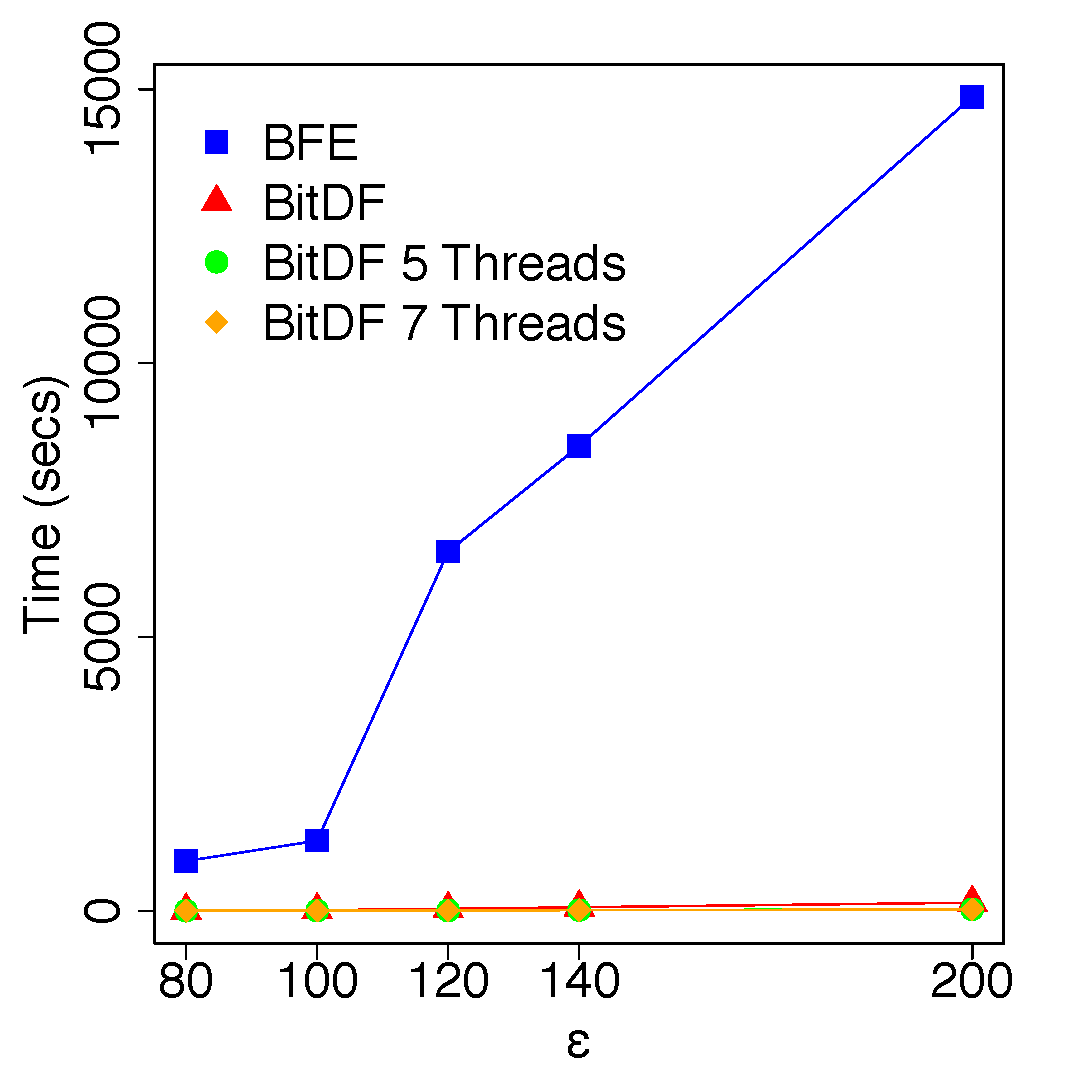
\includegraphics[width=\textwidth]{images/Brinkhoff_complete_varying_g.eps}
        \label{fig:brinkhoff_complete_vary_g}
    \end{subfigure}
    \footnotesize{Source: Made by the author.}
    \label{fig:brinkhoff_complete_results}
\end{figure*}

\begin{figure}[h!]
    \centering
    \caption{Results having $\delta = 8$, $\epsilon = 100$ and $\mu$ varying for the Brinkhoff dataset}
    \centerline{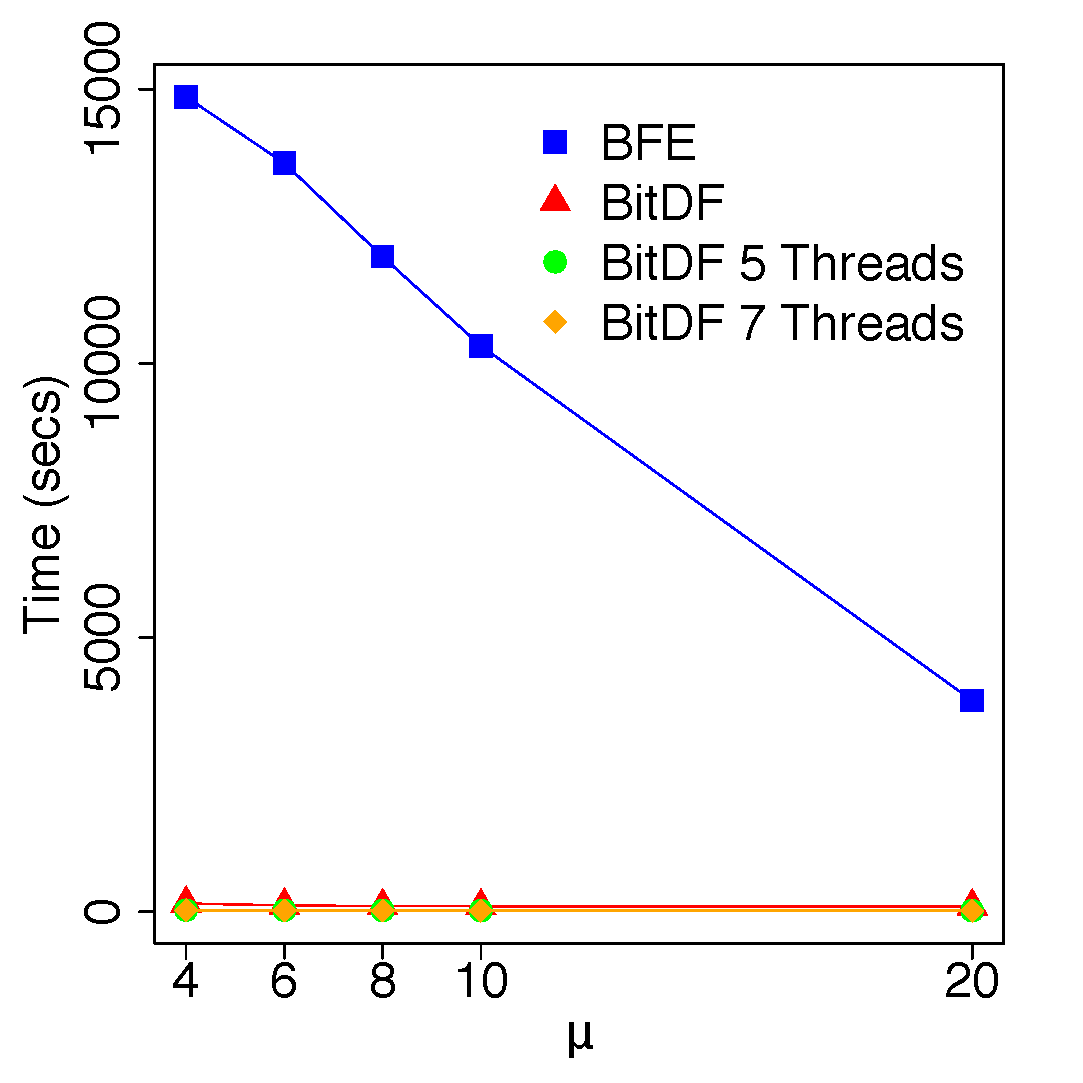
\includegraphics[width=0.5\textwidth]{images/Brinkhoff_complete_varying_n.eps}}
    \footnotesize{Source: Made by the author.}
    \label{fig:brinkhoff_complete_vary_n}
\end{figure}

In this section we could show that a somewhat simple remodeling in a system's architecture could lead to tremendous
running time improvements, by taking advantage of the multi-core paradigm. Our results show that we could reduce the
running time by as much as 96\%, when choosing the correct number of worker threads and the correct separation of work
that can be parallelized.

\chapter{Conclusion}
\label{chp:conclusion}
In this paper we propose a new efficient and elegant algorithm to find flock patterns, being able to work in on-line
environments.  Our results show that we outperformed state-of-the-art solutions by 99\% without compromising accuracy.
We prove our efficiency by performing experiments in 4 different datasets, bot real and synthetic.

This work opens some avenues for future advanced research studies, as follows: (1) apply BitDF to try to solve indoor
flock pattern detection; (2) focus on particularities in Smart Cities scenarios, such as traffic jam detection; (3)
conceptual design of a parallelizable model of BitDF in order to take full advantage of modern multicore architectures.


% References

\begin{references}
  \bibliography{references}
\end{references}

% Appendix

\theappendix
%\include{appendix/mapping-study}

\end{document}
